%% BUICS THESIS STYLE for LaTeX2e
%%
%% badwanpk, Tue March 10 18:53:15 2015
%%
%% PLEASE send improvements to badwanpk at bui dot edu dot pk
%%
%%========================================
%% Commands: pdflatex tese
%%           bibtex tese
%%           makeindex tese (only if creating an index) 
%%           pdflatex tese
%%========================================

\documentclass[11pt,a4paper]{report}
\usepackage[utf8]{inputenc}
\usepackage[english]{babel}
%\usepackage[portuges]{babel}
\usepackage{fancyvrb}
\usepackage{multirow}
%\usepackage{epstopdf}
\usepackage{rotating}
\usepackage{slashbox,pict2e}
\usepackage{soul}
\usepackage{amssymb}
\usepackage{lscape}
\usepackage{longtable}
\usepackage{makeidx}
\usepackage{amsmath}
\usepackage{multirow}
\usepackage{makecell}
\usepackage{wrapfig}
\usepackage{graphicx}
\usepackage{float}
\usepackage{setspace}
\usepackage{makecell}
%% For the final version, comment next line and uncomment the second line
%\usepackage[provisional,alpharefs]{buics}
\usepackage[numericrefs]{buics} %alpharefs

% Load hyperref last
% \usepackage[pdftex,plainpages=false,pdfpagelabels,bookmarks,hyperindex,hyperfigures]{hyperref}

%PDF properties 
\hypersetup{
  pdftitle={Nexora: A Modern Full-Stack Web Application},
  pdfauthor={Muhammad Ibrahim, Saim Zafar, Zarish Fatima},
  pdfsubject={Computer Science},
  pdfcreator={MiKTex 2.9},
  pdfproducer={MiKTex 2.9},
  pdfkeywords={Web Development, Full-Stack, Node.js, MySQL}
}

%% Options: 
%% - english: titles, etc in english
%% - provisional: the thesis has not been approved yet
%% - print: links are not shown (for paper versions)
%% - alpharefs: bibliography references are alphabetic
%% - numericrefs: bibliography references are numbered (in order of citation)
%% ( by default: author-date format of the ``natbib'' package is used 


%% Provide a version number in order to keep track of
%% thesis versions (it will printed in the footer of most pages)

\version{v1.0.2025}

%% uncomment in the final version in order to make version footer disappear
%\noversiontrue

%% uncomment to create an index (at the end of the document)
\makeindex 

%%  path to the figures directory
%%  TIP: use folder ``figures'' to keep all your figures
\graphicspath{{figures/}}

%%----------------------------------------
%% TIP: if you want to define more macros, use an external file to
%% keep them
%%----------------------------------------

%%========================================
%% Start of document
%%========================================
\begin{document}

%%----------------------------------------
%% Information about the work
%%----------------------------------------
\title{Nexora: A Modern Full-Stack Web Application}
\author{{\sc Muhammad Ibrahim}\\01-135241-035\\[1em]
{\sc Saim Zafar}\\01-135241-045\\[1em]
{\sc Zarish Fatima}\\01-135241-052}


\degree{\textbf{\Large{Bachelor of Science in Information Technology}}}

%\degree{\emph{Thesis submitted to the Department of Computer Science, Bahria University, Islamabad\\for fulfillment of the requirements of Bachelors of Science in Computer Science degree.}}
%% Date of submission

\department{Department of Computer Science\\Bahria University, Islamabad}
\thesisdate{December 2023}
%\thesisdate{\Large{\textbf{September 2012}}}

%% insert copyright text if used
\copyrightnotice{Muhammad Ibrahim, Saim Zafar, Zarish Fatima, 2025}

%% uncomment next line if necessary
%%\supervisor{Supervisor}{Supervisor Name}{}


% uncomment committee stuff in the final version if used

\certificatetext{We accept the work contained in the report titled ``Nexora: A Modern Full-Stack Web Application'', written by Muhammad Ibrahim, Saim Zafar, and Zarish Fatima as a confirmation to the required standard for the partial fulfillment of the degree of Bachelor of Science in Information Technology.}

\committeetext{Approved by \ldots:}

\committeemember{Teacher}{Sir Adnan Jelani}
\signature

\committeedate{May 30$^{st}$, 2025}

%% specify cover logo (in folder ``figures'')
\logo{BUI-Logo}

%%----------------------------------------
%% Cover page(s)
%%----------------------------------------
\maketitle
%% uncomment next line in the final version if used
\committeepage

%% Preliminary materials
\StartPrelim
\begin{singlespace}
  \chapter*{Abstract}

This thesis presents the development of Nexora, a modern full-stack web application designed as a comprehensive e-commerce platform. The project was developed by a team of three students from Bahria University, implementing advanced features for customers, vendors, and administrators.

The system architecture follows a three-tier design, utilizing Node.js and Express.js for the backend, MySQL for the database, and modern web technologies for the frontend. The implementation includes role-based access control, secure payment processing, real-time order tracking, and a comprehensive admin dashboard.

Key features of the platform include user authentication, product management, shopping cart functionality, order processing, and vendor management. The system is deployed across multiple cloud platforms including Render, Netlify, and Clever Cloud, ensuring high availability and scalability.

The project demonstrates the practical application of modern web development technologies and best practices in software engineering, including agile methodology, version control, and comprehensive testing strategies.  % the abstract
  \chapter*{Acknowledgments}

We would like to express our sincere gratitude to our supervisor for their invaluable guidance, support, and expertise throughout the development of this project. Their insights and feedback have been instrumental in shaping the direction and quality of our work.

We are also grateful to the faculty members of the Department of Computer Science at Bahria University for providing us with the knowledge and skills necessary to undertake this project. Their dedication to teaching and research has been a constant source of inspiration.

Special thanks to our families and friends for their unwavering support and understanding during the long hours spent on this project. Their encouragement has been crucial in helping us overcome challenges and maintain our motivation.

Finally, we would like to acknowledge the open-source community and the developers of the various tools and libraries that made this project possible. Their contributions to the field of software development have enabled us to build a modern and robust application.   % the acknowledgments
  \chapter*{Quote}

\begin{quote}
``The best way to predict the future is to implement it yourself.''
\begin{flushright}
--- Peter Drucker
\end{flushright}
\end{quote}     % initial quotation if desired
  \cleardoublepage
  \pdfbookmark[0]{Table of Contents}{contents}
  \tableofcontents
  \cleardoublepage
  \pdfbookmark[0]{List of Figures}{figures}
  \listoffigures
  \cleardoublepage
  \pdfbookmark[0]{List of Tables}{tables}
  \listoftables
  \chapter*{List of Abbreviations}

\begin{tabular}{ll}
API & Application Programming Interface \\
CDN & Content Delivery Network \\
CI/CD & Continuous Integration/Continuous Deployment \\
CSS & Cascading Style Sheets \\
DB & Database \\
ER & Entity-Relationship \\
HTML & HyperText Markup Language \\
HTTP & HyperText Transfer Protocol \\
JWT & JSON Web Token \\
ORM & Object-Relational Mapping \\
REST & Representational State Transfer \\
SQL & Structured Query Language \\
UI & User Interface \\
UX & User Experience \\
\end{tabular}   % the list of abbreviations used
\end{singlespace}

%%----------------------------------------
%% Body
%%----------------------------------------
\StartBody

%% TIP: use a separate  file for each
\chapter{Introduction}\label{chap:introduction}

\section{Project Overview}
Nexora is a modern full-stack web application developed as a thesis project by a team of three students from Bahria University. The project aims to create a comprehensive e-commerce platform with advanced features for customers, vendors, and administrators.

\section{Team Structure}
The project was developed by:
\begin{itemize}
    \item Muhammad Ibrahim (01-135241-035)
    \begin{itemize}
        \item Backend Development
        \item API Implementation
        \item Server Architecture
        \item Deployments
    \end{itemize}
    \item Saim Zafar (01-135241-045)
    \begin{itemize}
        \item Frontend Development
        \item User Interface Design
        \item Responsive Layout Implementation
    \end{itemize}
    \item Zarish Fatima (01-135241-052)
    \begin{itemize}
        \item Database Design
        \item System Integration
        \item Testing and Documentation
    \end{itemize}
\end{itemize}

\section{Project Objectives}
The main objectives of the project include:
\begin{itemize}
    \item Development of a modern e-commerce platform
    \item Implementation of role-based access control
    \item Creation of a responsive and user-friendly interface
    \item Integration of secure payment processing
    \item Implementation of real-time order tracking
    \item Development of vendor management system
    \item Creation of comprehensive admin dashboard
\end{itemize}

\section{Project Scope}
The project encompasses:
\begin{itemize}
    \item Customer Features:
    \begin{itemize}
        \item User registration and authentication
        \item Product browsing and searching
        \item Shopping cart and checkout
        \item Order tracking and history
        \item Wishlist management
        \item Product reviews and ratings
    \end{itemize}
    \item Vendor Features:
    \begin{itemize}
        \item Product management
        \item Order processing
        \item Sales analytics
        \item Inventory management
        \item Customer communication
    \end{itemize}
    \item Admin Features:
    \begin{itemize}
        \item User management
        \item Product oversight
        \item Order management
        \item System configuration
        \item Analytics and reporting
    \end{itemize}
\end{itemize}

\section{Technology Stack}
The project utilizes:
\begin{itemize}
    \item Frontend:
    \begin{itemize}
        \item HTML5, CSS3, JavaScript \cite{webdev2023}
        \item jQuery for DOM manipulation
        \item AJAX for API communication
    \end{itemize}
    \item Backend:
    \begin{itemize}
        \item Node.js runtime environment \cite{nodejs}
        \item Express.js web framework \cite{expressjs}
        \item MySQL database \cite{mysql}
        \item Sequelize ORM
    \end{itemize}
    \item Development Tools:
    \begin{itemize}
        \item Git for version control
        \item VS Code for development
        \item Postman for API testing
        \item MySQL Workbench for database management
    \end{itemize}
\end{itemize}

\section{Project Timeline}
The project was developed over a period of 3 months:
\begin{itemize}
    \item Phase 1 (Months 0-1):
    \begin{itemize}
        \item Requirements gathering
        \item System design
        \item Database schema design
    \end{itemize}
    \item Phase 2 (Months 1-2):
    \begin{itemize}
        \item Frontend development
        \item Backend implementation
        \item Database implementation
    \end{itemize}
    \item Phase 3 (Months 2-3):
    \begin{itemize}
        \item System integration
        \item Testing and debugging
        \item Documentation
        \item Deployment
    \end{itemize}
\end{itemize}

\section{Expected Outcomes}
The project aims to deliver:
\begin{itemize}
    \item A fully functional e-commerce platform
    \item Comprehensive documentation
    \item Source code and database schema
    \item User and admin manuals
    \item Test reports and results
\end{itemize}


\section{Deployment Platforms}
The deployment of Nexora utilized multiple modern cloud platforms to ensure high availability, scalability, and ease of access:
\begin{itemize}
    \item \textbf{Render}: Used for deploying the backend Node.js/Express server and MySQL database. Render provides managed services, automated deployments from Git repositories, and secure environment variable management.
    \item \textbf{Netlify}: Used for deploying the frontend static site. Netlify offers continuous deployment, global CDN, and easy integration with frontend frameworks, ensuring fast and reliable delivery of the user interface.
    \item \textbf{Clever Cloud}: Used for additional backend services and as a backup deployment platform. Clever Cloud provides scalable infrastructure, automated scaling, and monitoring for Node.js applications.
\end{itemize}
These platforms collectively enabled seamless CI/CD workflows, robust hosting, and efficient resource management for the project.
 % Introduction
\chapter{Literature Review}
\label{chap:literature}

\section{Web Development Technologies}
\subsection{Frontend Technologies}
\begin{itemize}
    \item HTML5 and CSS3:
    \begin{itemize}
        \item Modern web standards
        \item Responsive design capabilities
        \item Semantic markup
        \item CSS Grid and Flexbox
    \end{itemize}
    \item JavaScript:
    \begin{itemize}
        \item ES6+ features
        \item Asynchronous programming
        \item DOM manipulation
        \item Event handling
    \end{itemize}
    \item Bootstrap Framework:
    \begin{itemize}
        \item Responsive grid system
        \item Component library
        \item Utility classes
        \item Mobile-first approach
    \end{itemize}
\end{itemize}

\subsection{Backend Technologies}
\begin{itemize}
    \item Node.js:
    \begin{itemize}
        \item Event-driven architecture
        \item Non-blocking I/O
        \item NPM ecosystem
        \item Performance benefits
    \end{itemize}
    \item Express.js:
    \begin{itemize}
        \item Middleware support
        \item Routing system
        \item Error handling
        \item Template engines
    \end{itemize}
    \item MySQL:
    \begin{itemize}
        \item Relational database
        \item ACID compliance
        \item Transaction support
        \item Performance optimization
    \end{itemize}
\end{itemize}

\section{E-commerce Platforms}
\subsection{Existing Solutions}
\begin{itemize}
    \item Shopify:
    \begin{itemize}
        \item Platform architecture
        \item Feature set
        \item Pricing model
        \item Limitations
    \end{itemize}
    \item WooCommerce:
    \begin{itemize}
        \item WordPress integration
        \item Customization options
        \item Plugin ecosystem
        \item Performance considerations
    \end{itemize}
    \item Magento:
    \begin{itemize}
        \item Enterprise features
        \item Scalability
        \item Customization
        \item Resource requirements
    \end{itemize}
\end{itemize}

\subsection{Market Analysis}
\begin{itemize}
    \item Current Trends:
    \begin{itemize}
        \item Mobile commerce
        \item Social media integration
        \item Personalization
        \item Payment methods
    \end{itemize}
    \item User Expectations:
    \begin{itemize}
        \item Fast loading times
        \item Easy navigation
        \item Secure transactions
        \item Responsive design
    \end{itemize}
    \item Business Requirements:
    \begin{itemize}
        \item Inventory management
        \item Order processing
        \item Customer service
        \item Analytics
    \end{itemize}
\end{itemize}

\section{Security Considerations}
\subsection{Web Security}
\begin{itemize}
    \item Authentication:
    \begin{itemize}
        \item JWT implementation
        \item Password hashing
        \item Session management
        \item OAuth integration
    \end{itemize}
    \item Data Protection:
    \begin{itemize}
        \item SQL injection prevention
        \item XSS protection
        \item CSRF tokens
        \item Input validation
    \end{itemize}
    \item Secure Communication:
    \begin{itemize}
        \item HTTPS implementation
        \item SSL/TLS protocols
        \item Certificate management
        \item Secure headers
    \end{itemize}
\end{itemize}

\section{Performance Optimization}
\subsection{Frontend Optimization}
\begin{itemize}
    \item Loading Speed:
    \begin{itemize}
        \item Asset minification
        \item Image optimization
        \item Caching strategies
        \item Code splitting
    \end{itemize}
    \item User Experience:
    \begin{itemize}
        \item Responsive design
        \item Progressive loading
        \item Error handling
        \item Feedback mechanisms
    \end{itemize}
\end{itemize}

\subsection{Backend Optimization}
\begin{itemize}
    \item Database:
    \begin{itemize}
        \item Query optimization
        \item Indexing strategies
        \item Connection pooling
        \item Caching mechanisms
    \end{itemize}
    \item Server:
    \begin{itemize}
        \item Load balancing
        \item Resource management
        \item Error handling
        \item Monitoring
    \end{itemize}
\end{itemize}

\section{Research Methodology}
\subsection{Technology Selection}
\begin{itemize}
    \item Criteria:
    \begin{itemize}
        \item Performance requirements
        \item Scalability needs
        \item Development time
        \item Resource availability
    \end{itemize}
    \item Evaluation:
    \begin{itemize}
        \item Feature comparison
        \item Performance testing
        \item Security assessment
        \item Cost analysis
    \end{itemize}
\end{itemize}

\subsection{Implementation Strategy}
\begin{itemize}
    \item Development Approach:
    \begin{itemize}
        \item Agile methodology
        \item Version control
        \item Testing strategy
        \item Documentation
    \end{itemize}
    \item Quality Assurance:
    \begin{itemize}
        \item Code review process
        \item Testing procedures
        \item Performance monitoring
        \item Security auditing
    \end{itemize}
\end{itemize}

% Add technology comparison diagram
\begin{figure}[h]
    \centering
    \fbox{\parbox{0.8\textwidth}{
        \centering
        [Technology Stack Comparison Diagram]
    }}
    \caption{Technology Stack Comparison}
    \label{fig:technology-comparison}
\end{figure}  % Literature Review
\chapter{Requirements Specifications}

\section{Functional Requirements}
The following table outlines the main functional requirements for Nexora:

\begin{itemize}
    \item \textbf{User Authentication \& Role Management}
    \begin{itemize}
        \item FR-01: The system allows vendors, customers, and admins to create accounts and log in securely.
        \item FR-02: The system provides role-based access, restricting actions based on user type.
        \item FR-03: The system allows users to reset passwords through email verification.
    \end{itemize}
    \item \textbf{Vendor Management}
    \begin{itemize}
        \item FR-04: The system allows vendors to register, update, and delete their profiles.
        \item FR-05: The system enables vendors to add, edit, and remove products.
        \item FR-06: The system allows vendors to view and manage orders.
        \item FR-07: The system generates sales reports for vendors based on transactions.
    \end{itemize}
    \item \textbf{Product Management}
    \begin{itemize}
        \item FR-08: The system allows vendors to add products with images, descriptions, and prices.
        \item FR-09: The system enables customers to search for products using filters such as category, price, and rating.
        \item FR-10: The system displays product availability based on vendor stock levels.
    \end{itemize}
    \item \textbf{Shopping Cart \& Checkout}
    \begin{itemize}
        \item FR-11: The system allows customers to add, update, and remove items from the shopping cart.
        \item FR-12: The system displays the total price, including applicable taxes or discounts.
        \item FR-13: The system allows customers to proceed to check out and make payments securely.
        \item FR-14: The system generates a unique order ID for every purchase.
    \end{itemize}
    \item \textbf{Order Processing \& Tracking}
    \begin{itemize}
        \item FR-15: The system allows customers to track their order status (Pending, Shipped, Delivered).
        \item FR-16: The system notifies vendors when an order is placed and requires processing.
    \end{itemize}
    \item \textbf{Customer Reviews \& Ratings}
    \begin{itemize}
        \item FR-17: The system will allow customers to leave reviews and rate products.
        \item FR-18: The system shows an average rating for each product based on customer feedback.
        \item FR-19: The system allows admins to moderate and remove inappropriate reviews.
    \end{itemize}
    \item \textbf{Admin Management \& Marketplace Control}
    \begin{itemize}
        \item FR-20: The system allows the admin to approve or reject vendor registrations.
        \item FR-21: The system enables the admin to monitor and manage all users, products, and transactions.
        \item FR-22: The system provides sales analytics and reports to track marketplace performance.
    \end{itemize}
\end{itemize}

\clearpage
\section{Use Cases}

% Use Case: View Product Details
\begin{table}[h]
\centering
\renewcommand{\arraystretch}{1.2}
\begin{tabular}{|p{3cm}|p{10cm}|}
\hline
\textbf{Use Case Name} & View Product Details \\
\hline
\textbf{Actors} & Customer \\
\hline
\textbf{Description} & This use case allows customers to view detailed information about a product, including its description, price, images, and customer reviews. \\
\hline
\textbf{Preconditions} & The product must exist in the system and be available for viewing. \\
\hline
\textbf{Postconditions} & The system displays the product details. If the customer decides, they can add the product to their cart or submit a review. \\
\hline
\textbf{Main Flow} & \makecell[l]{1. Customer selects a product. \\ 2. System shows product details. \\ 3. Customer may enlarge images, read reviews, or add to cart.} \\
\hline
\textbf{Alternative Flow} & Product is Out of Stock: If the product is out of stock, the system displays "Out of Stock" instead of the Add to Cart button. The customer may choose to add the product to their Wishlist (if implemented in future versions). \\
\hline
\textbf{Exceptions} & \parbox[t]{10cm}{Product Not Found: If the selected product does not exist, the system displays "Product not available." \\ System Error: If there is an issue retrieving product details, the system displays "Unable to load product information. Please try again later."} \\
\hline
\end{tabular}
\caption{Use Case: View Product Details}
\end{table}

% Use Case: Manage Cart (Add/Remove Products)
\begin{table}[h]
\centering
\renewcommand{\arraystretch}{1.2}
\begin{tabular}{|p{3cm}|p{10cm}|}
\hline
\textbf{Use Case Name} & Manage Cart (Add/Remove Products) \\
\hline
\textbf{Actors} & Customer \\
\hline
\textbf{Description} & This use case allows customers to manage their shopping cart by adding or removing products before proceeding to checkout. \\
\hline
\textbf{Preconditions} & The customer must be logged in (if required for cart functionality). The selected product must be available in stock. \\
\hline
\textbf{Postconditions} & The cart is updated with the selected product(s). The total price is recalculated. \\
\hline
\textbf{Main Flow} & \textbf{Adding a Product to Cart:}
1. The customer selects a product and clicks "Add to Cart."
2. The system checks if the product is available in stock.
3. If available, the system adds the product to the cart and updates the total price.
4. The system displays a confirmation message.
\textbf{Removing a Product from Cart:}
1. The customer navigates to the Cart page.
2. The customer selects a product and clicks "Remove."
3. The system removes the product from the cart and updates the total price.
4. The system displays a confirmation message. \\
\hline
\textbf{Alternative Flow} & Adjusting Product Quantity: The customer selects a product and updates the quantity. The system recalculates the total price and updates the cart. \\
\hline
\textbf{Exceptions} & Product Out of Stock: If the product becomes unavailable after adding it to the cart, the system removes it and notifies the customer. System Error: If an issue occurs while updating the cart, the system displays an error message. \\
\hline
\end{tabular}
\caption{Use Case: Manage Cart (Add/Remove Products)}
\end{table}

% Use Case: Proceed to Checkout
\begin{table}[h]
\centering
\renewcommand{\arraystretch}{1.2}
\begin{tabular}{|p{3cm}|p{10cm}|}
\hline
\textbf{Use Case Name} & Proceed to Checkout \\
\hline
\textbf{Actors} & Customer \\
\hline
\textbf{Description} & This use case allows customers to proceed to checkout after selecting products in their cart. The system collects shipping and payment details before finalizing the purchase. \\
\hline
\textbf{Preconditions} & The customer must have at least one product in their cart. The selected products must be available in stock. \\
\hline
\textbf{Postconditions} & The order is successfully placed if payment is completed. The system generates an order ID and updates the order status. \\
\hline
\textbf{Main Flow} & \makecell[l]{1. Customer goes to cart and clicks Proceed to Checkout. \\ 2. System shows order summary. \\ 3. Customer enters shipping and payment info, confirms. \\ 4. System processes payment,creates order ,shows confirmation.} \\
\hline
\textbf{Alternative Flow} & \parbox[t]{10cm}{Applying Discount Code: The customer enters a discount code before making the payment. The system verifies and applies the discount if valid. The total amount is updated.} \\
\hline
\textbf{Exceptions} & \parbox[t]{10cm}{Cart is Empty: If the cart is empty, the system disables the checkout button and displays a message. \\ Payment Failure: If the payment fails, the system displays an error. \\ Product Out of Stock: If an item goes out of stock before checkout, the system removes it from the cart and notifies the customer.} \\
\hline
\end{tabular}
\caption{Use Case: Proceed to Checkout}
\end{table}

% Use Case: Track Order Status
\begin{table}[h]
\centering
\begin{tabular}{|p{3cm}|p{10cm}|}
\hline
\textbf{Use Case Name} & Track Order Status \\
\hline
\textbf{Actors} & Customer \\
\hline
\textbf{Description} & This use case allows customers to track the status of their orders, providing updates on processing, shipping, and delivery. \\
\hline
\textbf{Preconditions} & The customer must have placed at least one order. \\
\hline
\textbf{Postconditions} & The system displays the current order status. \\
\hline
\textbf{Main Flow} & 1. The customer directs to the Order History page. 2. The customer selects an order to view its details. 3. The system retrieves and displays the order details, including: Order ID, Order date and total price, Status (Processing, Shipped, Delivered), Estimated delivery date. 4. The customer can exit the order tracking page and then return to the main dashboard. \\
\hline
\textbf{Alternative Flow} & Order Status Updated: If the order status changes, the system automatically updates it in real-time and notifies the customer. \\
\hline
\textbf{Exceptions} & No Orders Found: If the customer has no orders, the system displays a message. System Error: If the system fails to retrieve order details, an error message is displayed. \\
\hline
\end{tabular}
\caption{Use Case: Track Order Status}
\end{table}

% Use Case: Submit Product Review
\begin{table}[h]
\centering
\begin{tabular}{|p{3cm}|p{10cm}|}
\hline
\textbf{Use Case Name} & Submit Product Review \\
\hline
\textbf{Actors} & Customer \\
\hline
\textbf{Description} & This use case allows customers to submit reviews and ratings for purchased products. The system verifies that the customer has bought the product before allowing them to submit a review. \\
\hline
\textbf{Preconditions} & The customer must have purchased the product. \\
\hline
\textbf{Postconditions} & The review is successfully submitted and displayed on the product page. \\
\hline
\textbf{Main Flow} & 1. The customer navigates to the Order History page. 2. The customer selects a purchased product and clicks Write a Review. 3. The system checks whether the customer has previously purchased the product. 4. If eligible, the system displays the review form. 5. The customer enters a rating and review and clicks Submit. 6. The system saves the review and updates the product page. 7. A confirmation message is displayed. \\
\hline
\textbf{Alternative Flow} & Edit or Delete Review: The customer can edit or delete a submitted review. The product page updates accordingly. \\
\hline
\textbf{Exceptions} & Customer Did Not Purchase Product: The system displays a message if the customer tries to review a product they have not bought. System Error: If a system issue occurs while saving the review, an error message is displayed. \\
\hline
\end{tabular}
\caption{Use Case: Submit Product Review}
\end{table}

% Use Case: Vendor Registration
\begin{table}[h]
\centering
\begin{tabular}{|p{3cm}|p{10cm}|}
\hline
\textbf{Use Case Name} & Vendor Registration \\
\hline
\textbf{Actors} & Vendor \\
\hline
\textbf{Description} & This use case allows a vendor to register an account to sell products on the marketplace. The system verifies the provided details and requires admin approval before activation. \\
\hline
\textbf{Preconditions} & The vendor must provide valid registration details. \\
\hline
\textbf{Postconditions} & The vendor account is created and sent for admin approval. The vendor can log in only after approval. \\
\hline
\textbf{Main Flow} & 1. The vendor goes through the Vendor Registration page. 2. The vendor enters the required details. 3. The system validates the entered details. 4. If all information is correct, the system creates the vendor account. 5. The system notifies the admin for approval. 6. The vendor receives a confirmation message. \\
\hline
\textbf{Alternative Flow} & Admin Approves Registration: The admin reviews the vendor's application. If approved, the system activates the account, and the vendor is notified. \\
\hline
\textbf{Exceptions} & Email Already Registered: The system displays a message if the email is already in use. Missing Required Information: The system prompts the vendor to fill required fields. Admin Rejects Registration: The system notifies the vendor with the reason for rejection. \\
\hline
\end{tabular}
\caption{Use Case: Vendor Registration}
\end{table}

% Use Case: Add/Edit/Delete Product
\begin{table}[h]
\centering
\begin{tabular}{|p{3cm}|p{10cm}|}
\hline
\textbf{Use Case Name} & Add/Edit/Delete Product \\
\hline
\textbf{Actors} & Vendor \\
\hline
\textbf{Description} & This use case allows vendors to add new products, edit existing product details, or remove products from their listings. \\
\hline
\textbf{Preconditions} & The vendor must be logged into their account. \\
\hline
\textbf{Postconditions} & The product listing is updated in the system. \\
\hline
\textbf{Main Flow} & Adding a Product: 1. The vendor goes through the Product Management section. 2. The vendor clicks "Add New Product." 3. The vendor enters product details. 4. The system validates and saves the product. 5. The product is added to the vendor's store. Editing a Product: 1. The vendor selects a product. 2. The vendor clicks "Edit." 3. The vendor modifies details. 4. The system updates the product. Deleting a Product: 1. The vendor selects a product to delete. 2. The vendor clicks Delete. 3. The system asks for confirmation. 4. If confirmed, the system removes the product. \\
\hline
\textbf{Exceptions} & Missing Required Fields: The system prompts the vendor to complete the form. Product Not Found: The system displays a message if the product no longer exists. System Error: The system displays an error if changes cannot be saved. \\
\hline
\end{tabular}
\caption{Use Case: Add/Edit/Delete Product}
\end{table}

% Use Case: Manage Orders
\begin{table}[h]
\centering
\begin{tabular}{|p{3cm}|p{10cm}|}
\hline
\textbf{Use Case Name} & Manage Orders \\
\hline
\textbf{Actors} & Vendor \\
\hline
\textbf{Description} & This use case allows vendors to view, process, and update the status of customer orders. \\
\hline
\textbf{Preconditions} & The vendor must be logged into their account. At least one order must exist in the system. \\
\hline
\textbf{Postconditions} & The order status is updated in the system. Customers are notified of any changes to their order status. \\
\hline
\textbf{Main Flow} & 1. The vendor goes to the Orders Dashboard. 2. The system displays a list of orders. 3. The vendor selects an order to manage. 4. The vendor can view order details, update order status, or cancel order. 5. The system saves changes and updates the customer. \\
\hline
\textbf{Alternative Flow} & Order Partially Processed: The vendor can mark certain items as Shipped, while others remain Processing. The system updates the order details accordingly. \\
\hline
\textbf{Exceptions} & Order Not Found: The system displays a message if the order is not available. System Error: The system displays an error if order status cannot be updated. \\
\hline
\end{tabular}
\caption{Use Case: Manage Orders}
\end{table}

% Use Case: Approve/Reject Vendor Registration
\begin{table}[h]
\centering
\begin{tabular}{|p{3cm}|p{10cm}|}
\hline
\textbf{Use Case Name} & Approve/Reject Vendor Registration \\
\hline
\textbf{Actors} & Admin \\
\hline
\textbf{Description} & This use case allows the admin to review vendor registration requests and either approve or reject them based on verification criteria. \\
\hline
\textbf{Preconditions} & The vendor must have submitted a registration request. \\
\hline
\textbf{Postconditions} & If approved, the vendor account is activated, and they can log in. If rejected, the vendor is notified with the reason for rejection. \\
\hline
\textbf{Main Flow} & 1. The admin logs into the system and goes through the Vendor Approval Dashboard. 2. The system displays a list of pending vendor applications. 3. The admin selects a vendor application to review. 4. The admin checks the provided details. 5. The admin chooses to approve or reject the registration. \\
\hline
\textbf{Alternative Flow} & Request More Information: The admin can request additional information from the vendor. The system keeps the registration in a Pending state until all required details are submitted. \\
\hline
\textbf{Exceptions} & Vendor Already Approved: The system displays a message if the vendor is already active. System Error: The system displays an error if the request cannot be processed. \\
\hline
\end{tabular}
\caption{Use Case: Approve/Reject Vendor Registration}
\end{table}

% Use Case: Manage Users (Block/Unblock Vendors \& Customers)
\begin{table}[h]
\centering
\begin{tabular}{|p{3cm}|p{10cm}|}
\hline
\textbf{Use Case Name} & Manage Users (Block/Unblock Vendors \& Customers) \\
\hline
\textbf{Actors} & Admin \\
\hline
\textbf{Description} & This use case allows the admin to manage user accounts by blocking or unblocking vendors and customers based on violations or inactivity. \\
\hline
\textbf{Preconditions} & The user must have an active account in the system. \\
\hline
\textbf{Postconditions} & If blocked, the user cannot log in or access the system. If unblocked, the user regains access to their account. \\
\hline
\textbf{Main Flow} & 1. The admin logs into the system and navigates to the User Management Panel. 2. The system displays a list of registered users. 3. The admin selects a user account to manage. 4. The admin chooses to block or unblock the user. 5. The system updates the user status and notifies them via email. \\
\hline
\textbf{Alternative Flow} & Temporary Suspension: The admin can suspend the account for a specific period. The system sets an expiration date for the suspension. The user will automatically regain access after the suspension period ends. \\
\hline
\textbf{Exceptions} & User Already Blocked: The system displays a message if the user is already blocked. User Not Found: The system displays a message if the user does not exist. System Error: The system displays an error if the user status cannot be updated. \\
\hline
\end{tabular}
\caption{Use Case: Manage Users (Block/Unblock Vendors \& Customers)}
\end{table}

\begin{figure}[h]
    \centering
    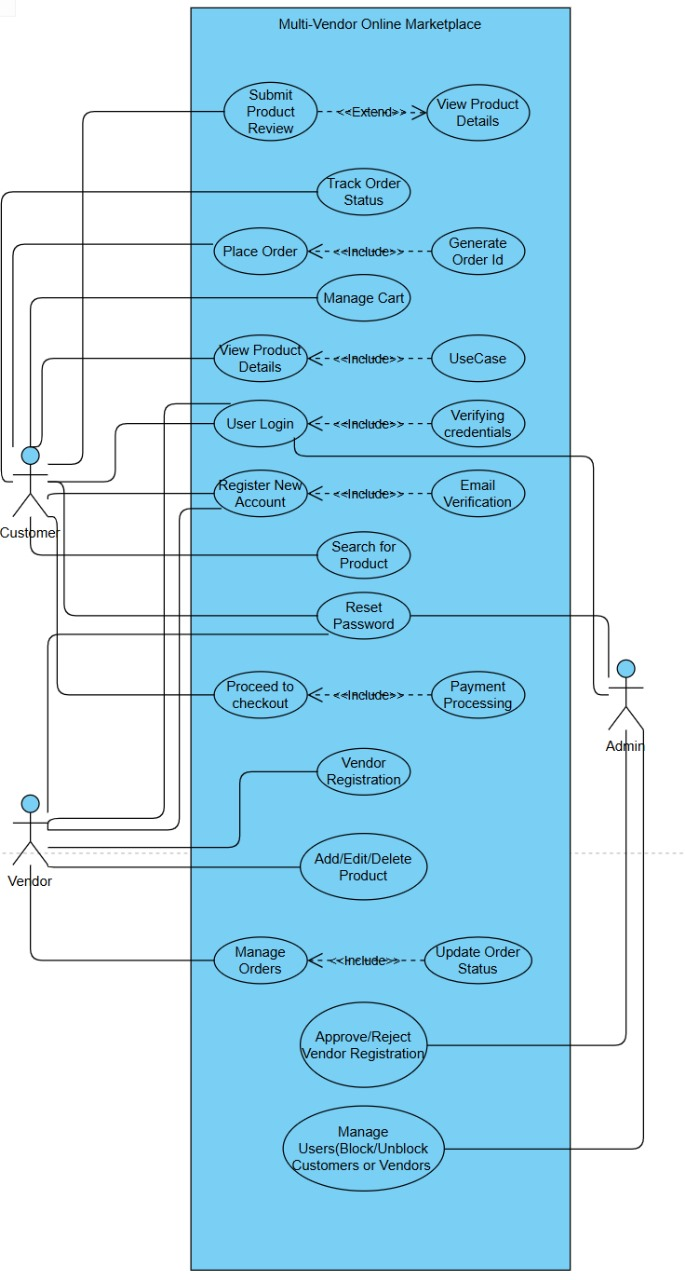
\includegraphics[width=0.9\textwidth]{UseCaseDiagram.jpg}
    \caption{Use Case Diagram for Nexora}
    \label{fig:use-case-diagram}
\end{figure}

\clearpage
\section{Non-Functional Requirements}
The following table outlines the main non-functional requirements for Nexora:

\begin{itemize}
    \item \textbf{Performance}
    \begin{itemize}
        \item NFR-01: The system will handle at least 50 simultaneous users without significant slowdown.
        \item NFR-02: Page load time should not exceed 3 seconds under normal usage conditions.
    \end{itemize}
    \item \textbf{Security}
    \begin{itemize}
        \item NFR-03: User passwords will be securely stored using encryption.
        \item NFR-04: All sensitive data shall be transmitted over HTTPS.
    \end{itemize}
    \item \textbf{Usability}
    \begin{itemize}
        \item NFR-05: The system has a simple and intuitive interface for ease of navigation.
        \item NFR-06: Customers are able to complete a purchase in no more than 5 steps.
    \end{itemize}
    \item \textbf{Scalability}
    \begin{itemize}
        \item NFR-07: The system will allow for future expansion, supporting additional vendors and products.
    \end{itemize}
    \item \textbf{Availability}
    \begin{itemize}
        \item NFR-08: The system maintains an uptime of at least 99\%.
    \end{itemize}
\end{itemize}

\section{Technical Requirements}
\subsection{Frontend}
\begin{itemize}
    \item HTML5, CSS3, JavaScript
    \item Responsive design framework
    \item Modern browser compatibility
    \item Progressive enhancement
\end{itemize}

\subsection{Backend}
\begin{itemize}
    \item Node.js runtime
    \item Express.js framework
    \item RESTful API design
    \item Database integration
\end{itemize}

\subsection{Database}
\begin{itemize}
    \item MySQL database
    \item Data normalization
    \item Indexing strategy
    \item Backup procedures
\end{itemize}

\section{Integration Requirements}
\begin{itemize}
    \item Payment gateway integration
    \item Email service integration
    \item File storage integration
    \item Analytics integration
\end{itemize}

\section{Compliance Requirements}
\begin{itemize}
    \item Data protection regulations
    \item Security standards
    \item Accessibility guidelines
    \item Industry best practices
\end{itemize}  % Requirements Specifications
\chapter{System Design}

\section{System Architecture}
\subsection{Overview}
The Nexora e-commerce platform follows a three-tier architecture:
\begin{itemize}
    \item Presentation Layer (Frontend)
    \item Application Layer (Backend)
    \item Data Layer (Database)
\end{itemize}

\begin{figure}[h]
    \centering
    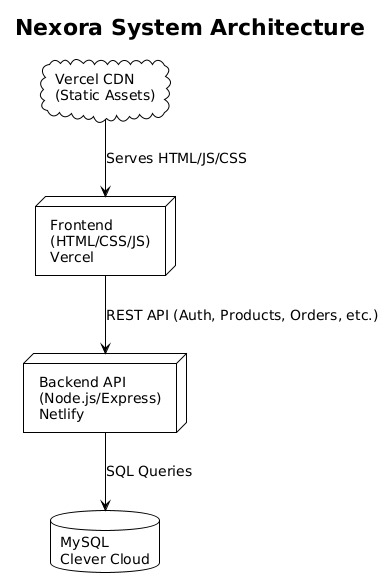
\includegraphics[width=0.8\textwidth]{SystemArchitecture.jpg}
    \caption{System Architecture Overview}
    \label{fig:system-architecture}
\end{figure}

\subsection{Component Diagram}
\begin{itemize}
    \item Frontend Components:
    \begin{itemize}
        \item User Interface
        \item Client-side Logic
        \item API Integration
    \end{itemize}
    \item Backend Components:
    \begin{itemize}
        \item API Server
        \item Business Logic
        \item Authentication Service
        \item File Service
    \end{itemize}
    \item Database Components:
    \begin{itemize}
        \item Data Storage
        \item Query Engine
        \item Backup System
    \end{itemize}
\end{itemize}

\section{Frontend Architecture}
\subsection{Component Structure}
\begin{itemize}
    \item Pages:
    \begin{itemize}
        \item Home
        \item Product Listing
        \item Product Details
        \item Cart
        \item Checkout
        \item User Dashboard
        \item Admin Panel
    \end{itemize}
    \item Components:
    \begin{itemize}
        \item Navigation
        \item Product Cards
        \item Forms
        \item Modals
        \item Notifications
    \end{itemize}
\end{itemize}

\begin{figure}[h]
    \centering
    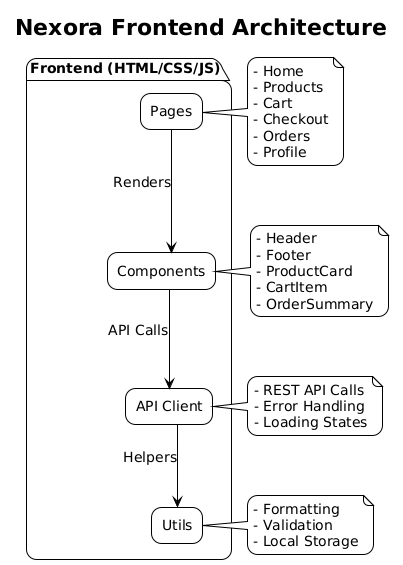
\includegraphics[width=0.8\textwidth]{FrontendArchitecture.png}
    \caption{Frontend Architecture}
    \label{fig:frontend-architecture}
\end{figure}

\section{Backend Architecture}
\subsection{API Design}
\begin{itemize}
    \item RESTful Endpoints
    \item Resource-based Routing
    \item Middleware Pipeline
    \item Error Handling
\end{itemize}

\subsection{Service Layer}
\begin{itemize}
    \item Authentication Service
    \item Product Service
    \item Order Service
    \item User Service
    \item File Service
\end{itemize}

\begin{figure}[h]
    \centering
    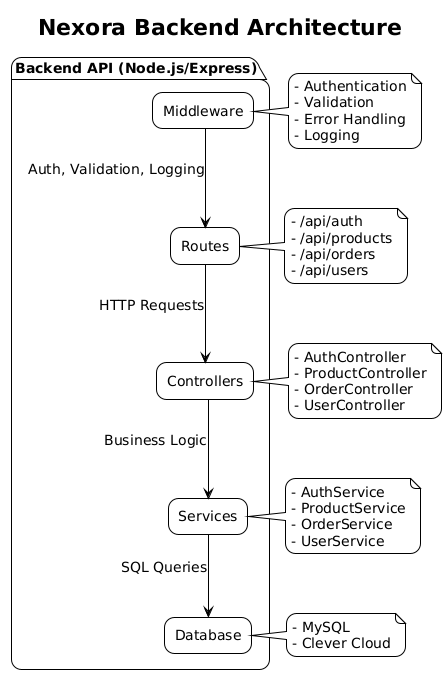
\includegraphics[width=0.8\textwidth]{BackendArchitecture.png}
    \caption{Backend Architecture}
    \label{fig:backend-architecture}
\end{figure}

\section{Database Design}
\subsection{Entity Relationship Diagram}
\begin{itemize}
    \item Core Entities:
    \begin{itemize}
        \item Users
        \item Products
        \item Orders
        \item Categories
    \end{itemize}
    \item Relationships:
    \begin{itemize}
        \item User-Order (1:N)
        \item Product-Category (M:N)
        \item Order-Product (M:N)
    \end{itemize}
\end{itemize}

\begin{figure}[h]
    \centering
    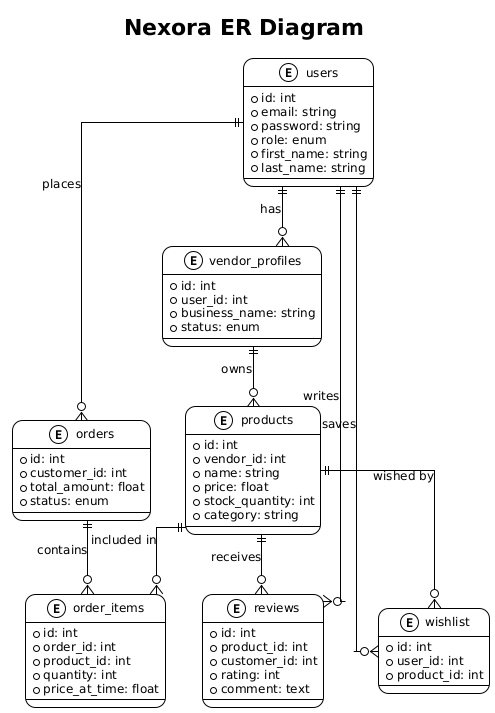
\includegraphics[width=0.8\textwidth]{ER_DiagramDetailed.png}
    \caption{Entity-Relationship Diagram}
    \label{fig:er-diagram}
\end{figure}

\section{Class Diagram}
\subsection{Core Classes}
\begin{itemize}
    \item User:
    \begin{itemize}
        \item Properties: id, name, email, role
        \item Methods: register(), login(), updateProfile()
    \end{itemize}
    \item Product:
    \begin{itemize}
        \item Properties: id, name, price, description
        \item Methods: create(), update(), delete()
    \end{itemize}
    \item Order:
    \begin{itemize}
        \item Properties: id, userId, total, status
        \item Methods: create(), updateStatus(), calculateTotal()
    \end{itemize}
\end{itemize}

\begin{figure}[h]
    \centering
    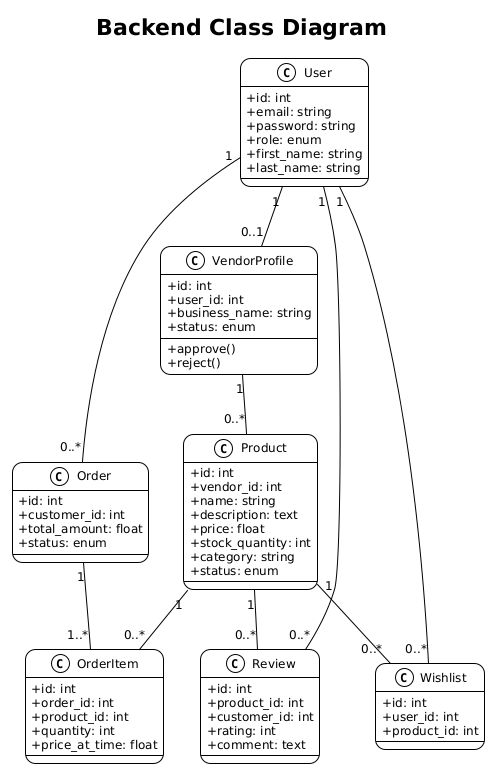
\includegraphics[width=0.8\textwidth]{DetailedClassDiagram.png}
    \caption{Detailed Class Diagram}
    \label{fig:class-diagram}
\end{figure}

\section{Sequence Diagrams}
\begin{figure}[h]
    \centering
    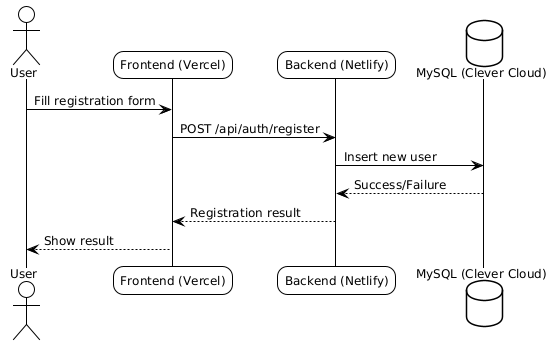
\includegraphics[width=0.7\textwidth]{Sequence_DiagramUsee_Registration.png}
    \caption{Sequence Diagram: User Registration}
    \label{fig:sd-registration}
\end{figure}

\begin{figure}[h]
    \centering
    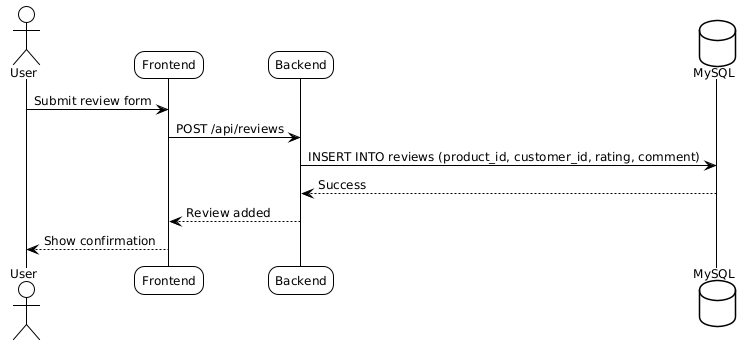
\includegraphics[width=0.7\textwidth]{SDWriteReview.png}
    \caption{Sequence Diagram: Write Review}
    \label{fig:sd-write-review}
\end{figure}

\begin{figure}[h]
    \centering
    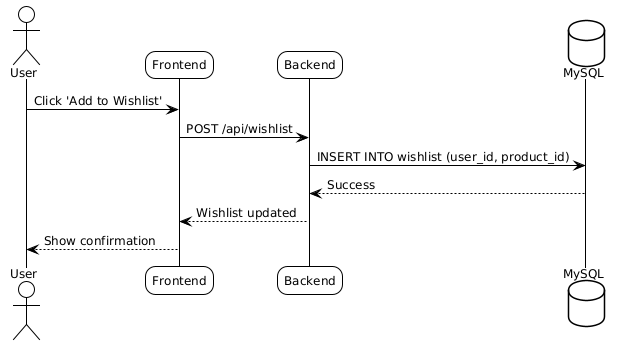
\includegraphics[width=0.7\textwidth]{SDAddtoWishlist.png}
    \caption{Sequence Diagram: Add to Wishlist}
    \label{fig:sd-add-wishlist}
\end{figure}

\begin{figure}[h]
    \centering
    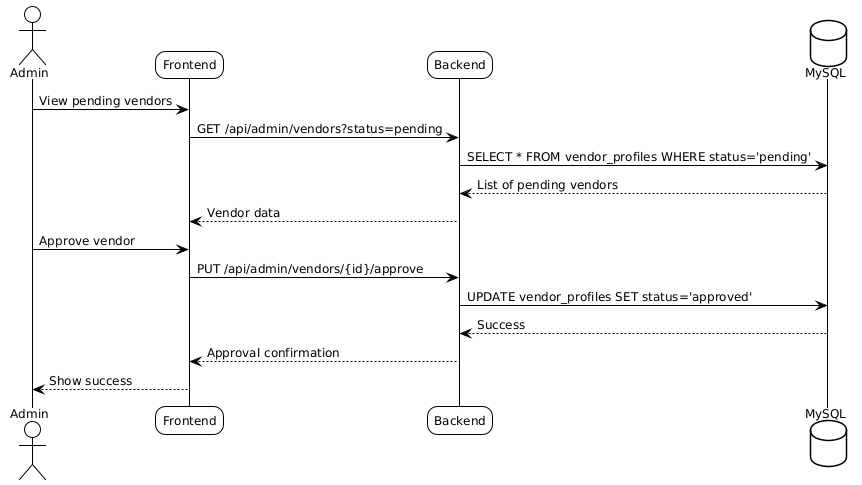
\includegraphics[width=0.7\textwidth]{SDVendor Approval.png}
    \caption{Sequence Diagram: Vendor Approval}
    \label{fig:sd-vendor-approval}
\end{figure}

\begin{figure}[h]
    \centering
    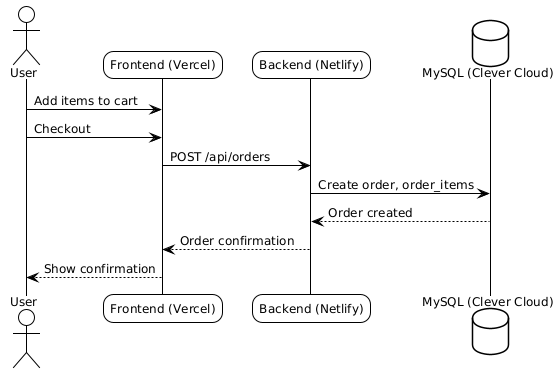
\includegraphics[width=0.7\textwidth]{Place_Order.png}
    \caption{Sequence Diagram: Place Order}
    \label{fig:sd-place-order}
\end{figure}

\section{Security Design}
\subsection{Authentication}
\begin{itemize}
    \item JWT-based authentication
    \item Password hashing
    \item Session management
    \item Role-based access control
\end{itemize}

\subsection{Data Protection}
\begin{itemize}
    \item Input validation
    \item SQL injection prevention
    \item XSS protection
    \item CSRF protection
\end{itemize}

\section{Performance Considerations}
\subsection{Optimization Strategies}
\begin{itemize}
    \item Caching:
    \begin{itemize}
        \item Browser caching
        \item API response caching
        \item Database query caching
    \end{itemize}
    \item Load Balancing:
    \begin{itemize}
        \item Horizontal scaling
        \item Request distribution
        \item Session management
    \end{itemize}
    \item Database Optimization:
    \begin{itemize}
        \item Indexing
        \item Query optimization
        \item Connection pooling
    \end{itemize}
\end{itemize}

\section{Deployment Architecture}
\subsection{Infrastructure}
\begin{itemize}
    \item Web Server
    \item Application Server
    \item Database Server
    \item File Storage
\end{itemize}

\subsection{Monitoring}
\begin{itemize}
    \item Performance monitoring
    \item Error tracking
    \item User analytics
    \item Security monitoring
\end{itemize}
 % System Design
\chapter{Frontend Implementation}

\section{Overview}
The frontend of Nexora is built using HTML, CSS, and JavaScript, following a component-based architecture for better maintainability and reusability.

\section{Technologies Used}
\begin{itemize}
    \item HTML5 and CSS3
    \item JavaScript (ES6+)
    \item Bootstrap for responsive design
    \item jQuery for DOM manipulation
    \item AJAX for API communication
\end{itemize}

\section{Key Features}
\begin{itemize}
    \item Responsive Design:
    \begin{itemize}
        \item Mobile-first approach
        \item Cross-browser compatibility
        \item Intuitive navigation
        \item Modern UI components
    \end{itemize}
    \item User Experience:
    \begin{itemize}
        \item Fast page loading
        \item Smooth interactions
        \item Clear feedback
        \item Error handling
    \end{itemize}
    \item Integration with Backend:
    \begin{itemize}
        \item API calls for data retrieval
        \item Authentication and authorization
        \item Real-time updates
    \end{itemize}
\end{itemize}

\section{UI/UX}
% Add screenshots or diagrams here in logical order:
% Landing Page -> Authentication -> User -> Checkout -> Vendor -> Admin

% --- Landing Page ---
\begin{figure}[htbp]
\centering
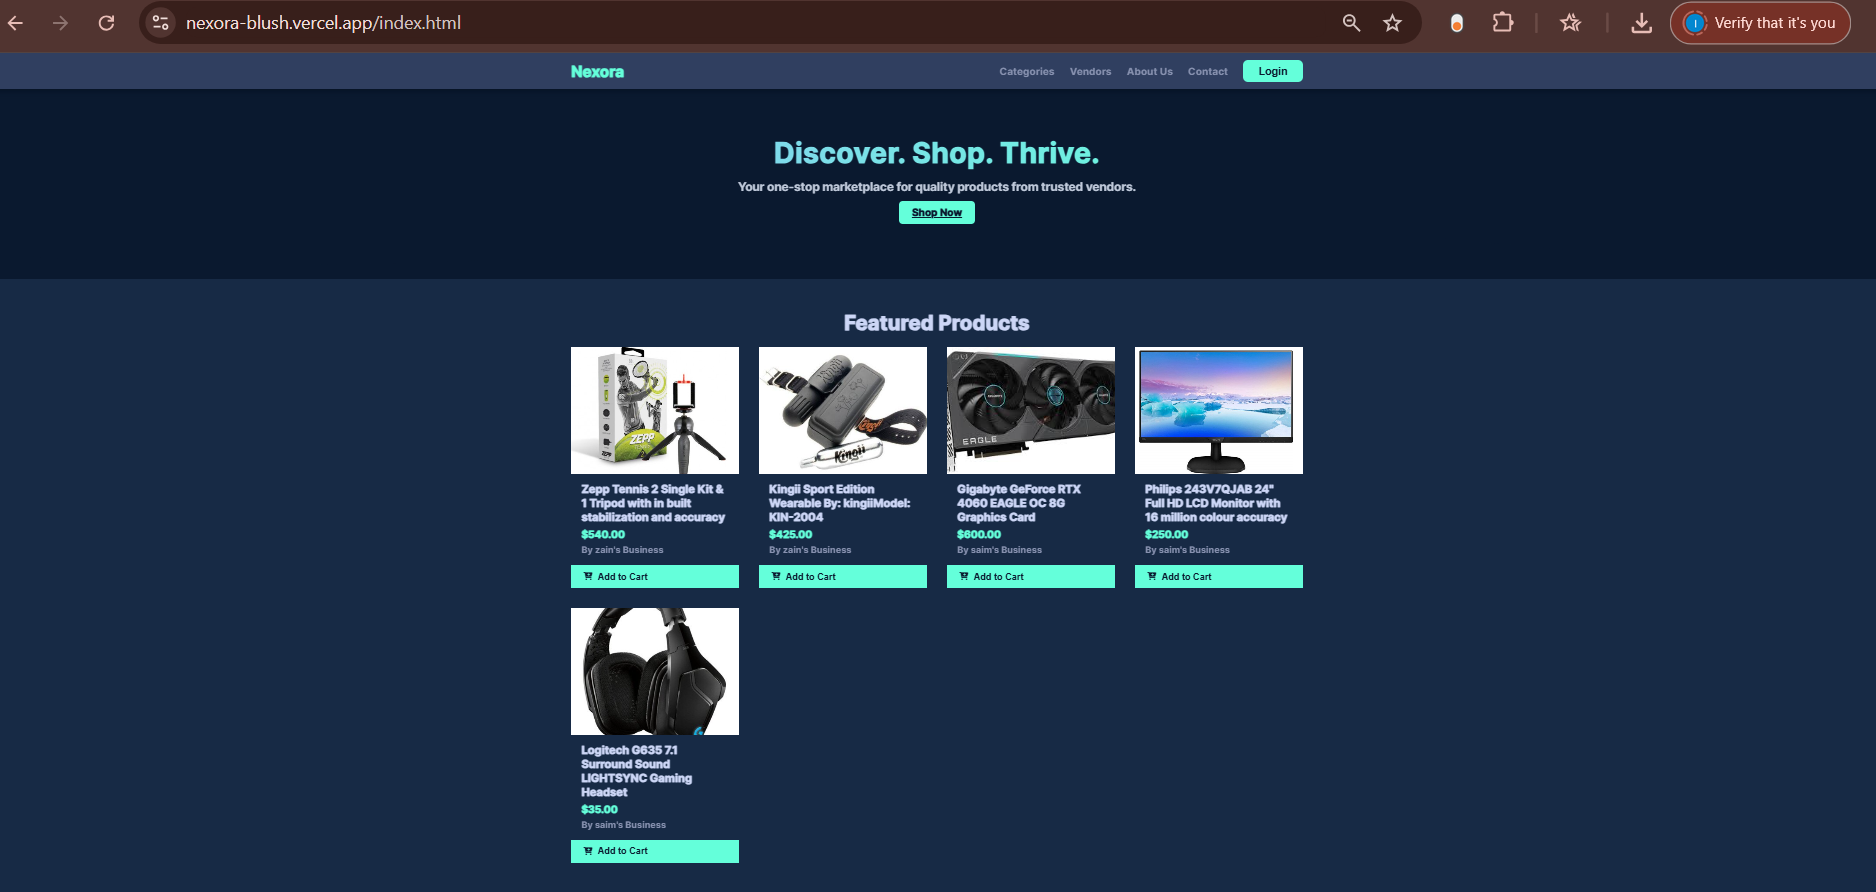
\includegraphics[width=\textwidth,keepaspectratio]{thesis/figures/Landing-Page.png}
\caption{Landing Page}
\label{fig:landing-page}
\end{figure}

% --- Authentication ---
\begin{figure}[htbp]
\centering
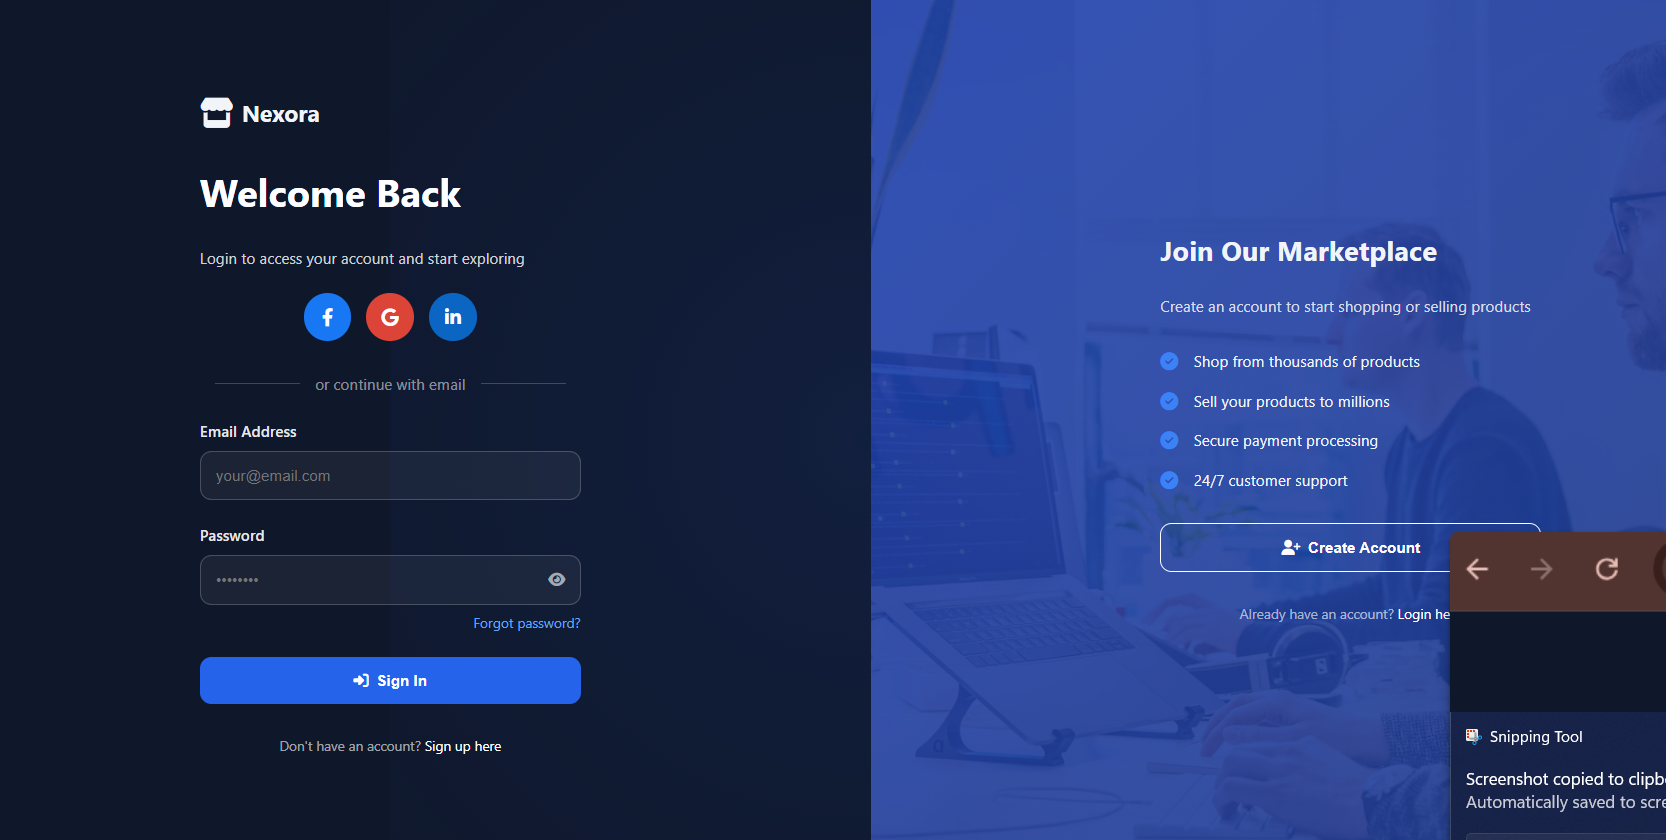
\includegraphics[width=\textwidth,keepaspectratio]{thesis/figures/Login-Registration.png}
\caption{Login and Registration Pages}
\label{fig:login-register}
\end{figure}

\begin{figure}[htbp]
\centering
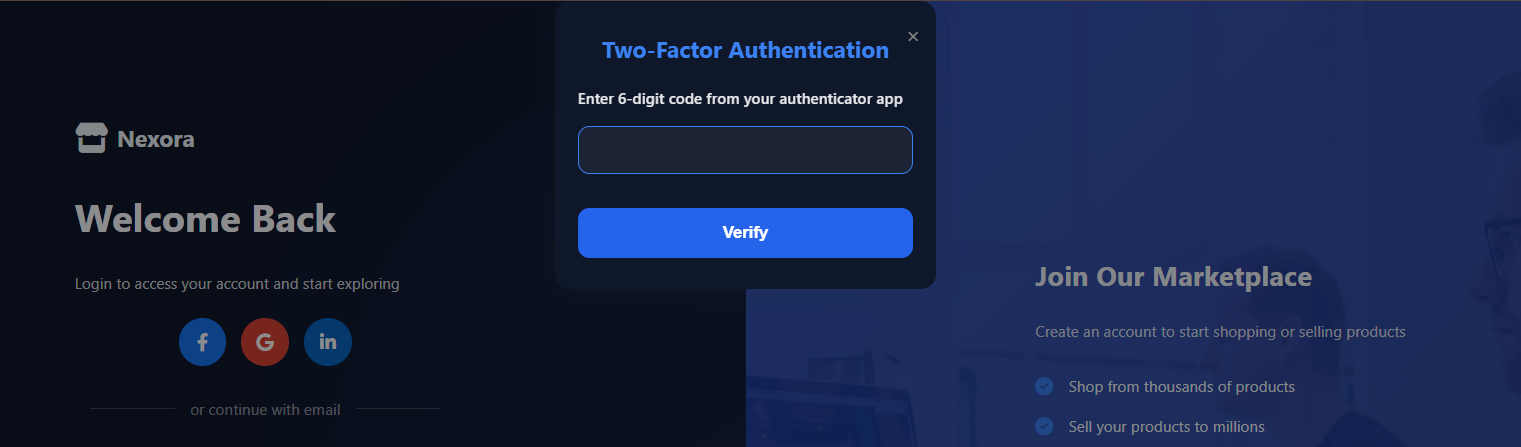
\includegraphics[width=\textwidth,keepaspectratio]{thesis/figures/2Fa.png}
\caption{2FA Authentication}
\label{fig:2fa}
\end{figure}

% --- User Interface ---
\begin{figure}[htbp]
\centering
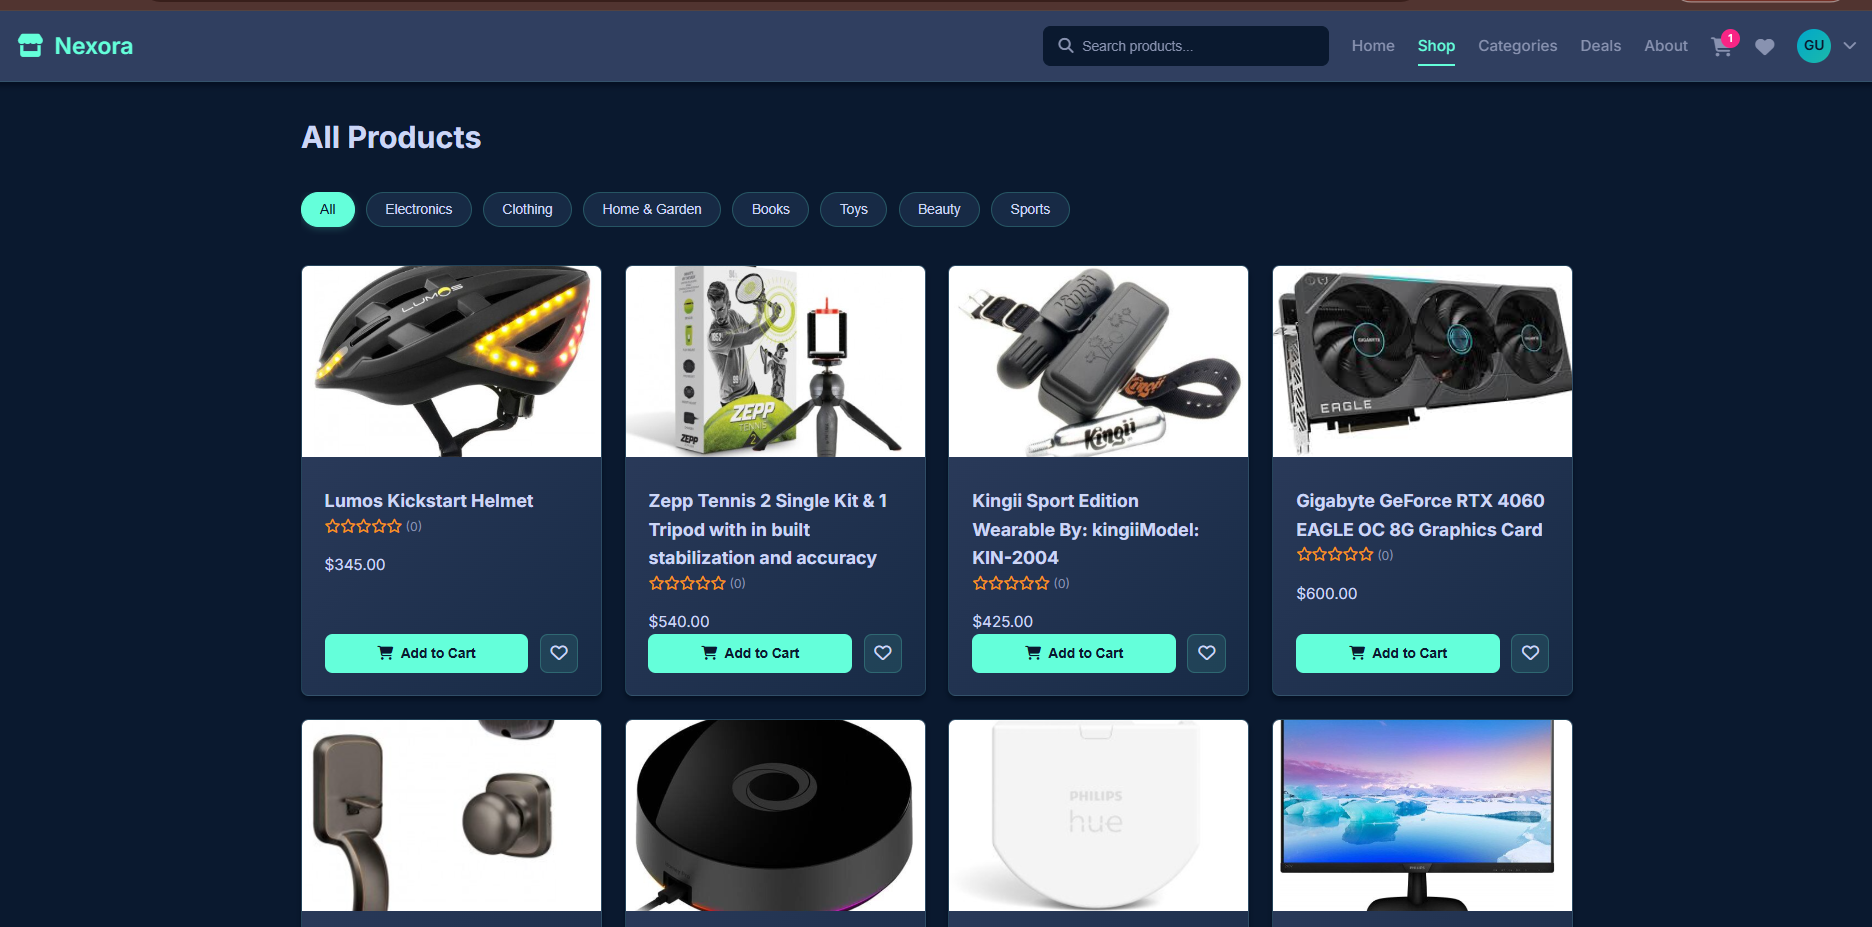
\includegraphics[width=\textwidth,keepaspectratio]{thesis/figures/User-Dashboard.png}
\caption{User Dashboard}
\label{fig:user-dashboard}
\end{figure}

\begin{figure}[htbp]
\centering
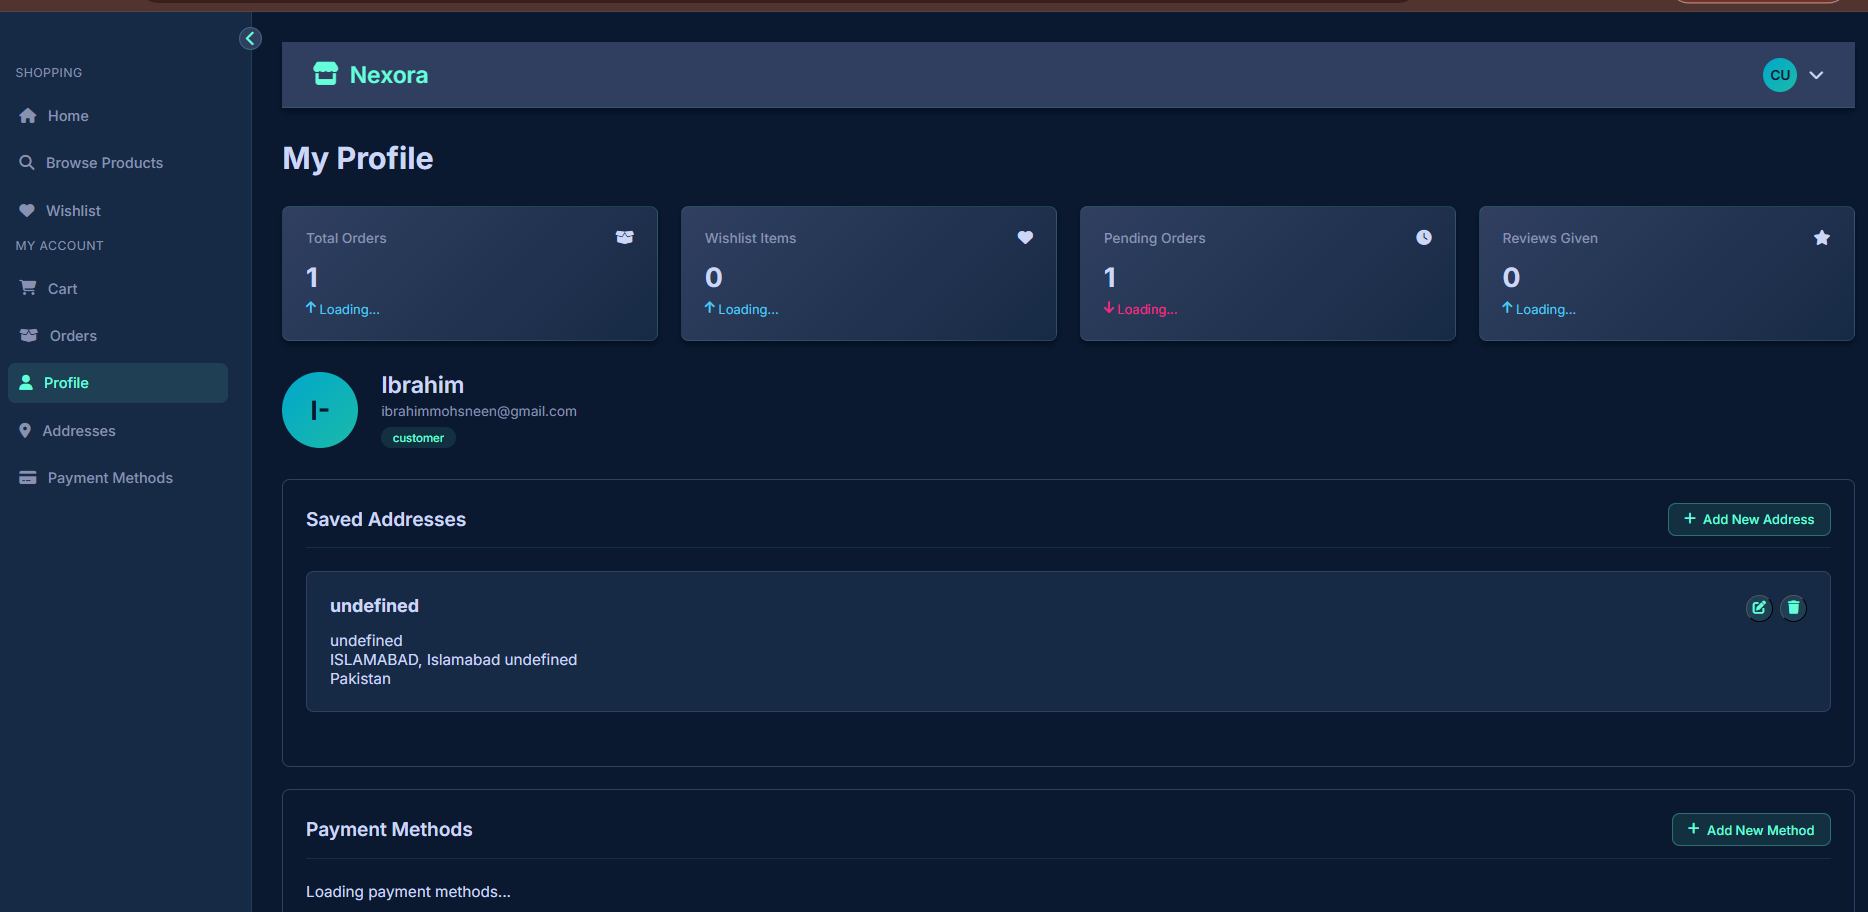
\includegraphics[width=\textwidth,keepaspectratio]{thesis/figures/User-Profile.png}
\caption{User Profile}
\label{fig:user-profile}
\end{figure}

% --- Checkout ---
\begin{figure}[htbp]
\centering
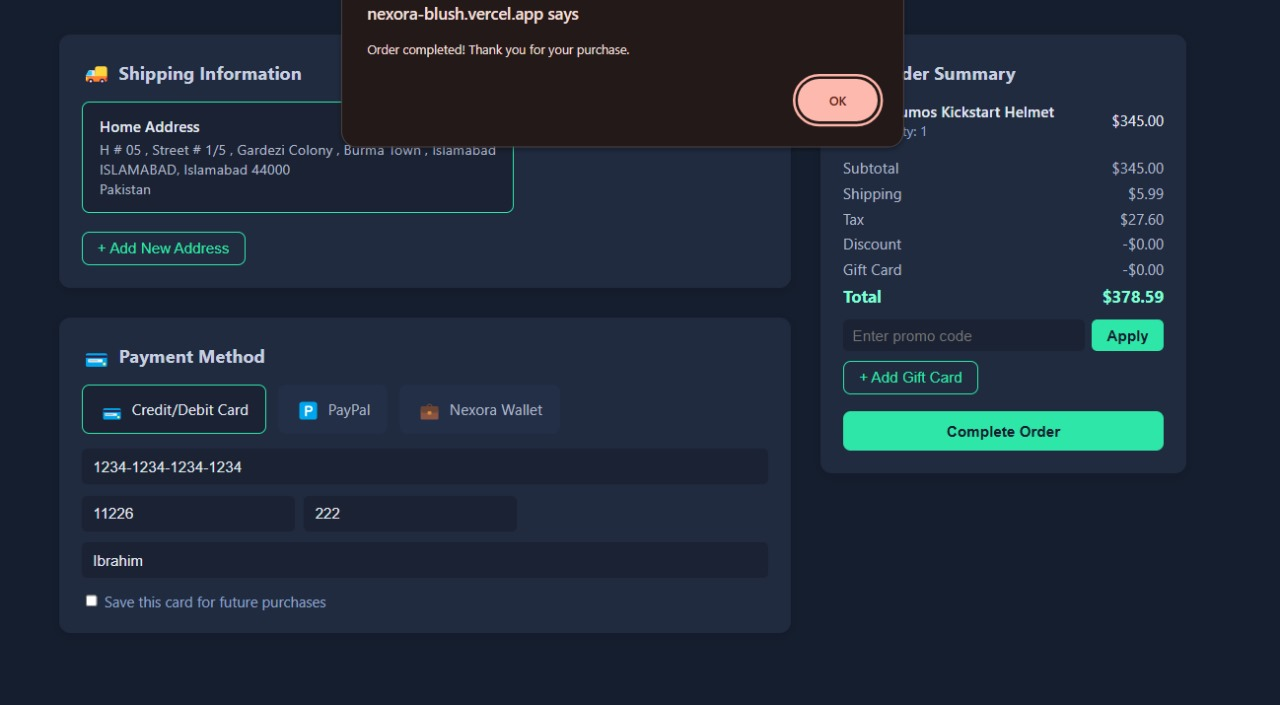
\includegraphics[width=\textwidth,keepaspectratio]{thesis/figures/Checkout.jpg}
\caption{Checkout Process}
\label{fig:checkout}
\end{figure}

% --- Vendor Interface ---
\begin{figure}[htbp]
\centering
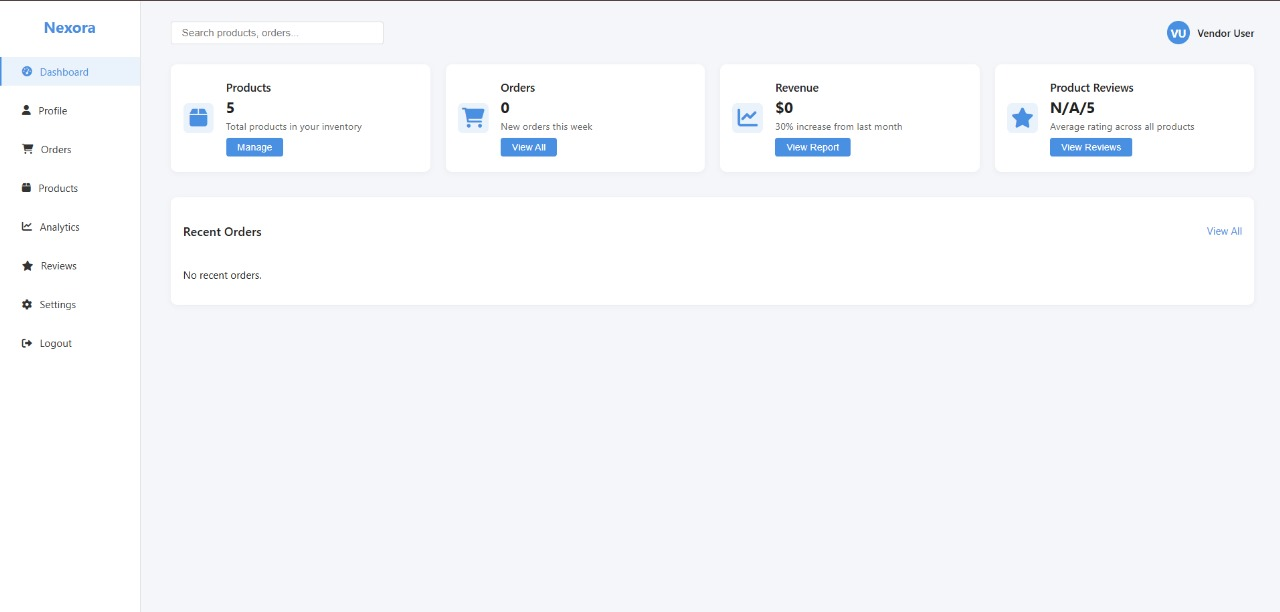
\includegraphics[width=\textwidth,keepaspectratio]{thesis/figures/Vendor-Dashboard.jpg}
\caption{Vendor Dashboard}
\label{fig:vendor-dashboard}
\end{figure}

\begin{figure}[htbp]
\centering
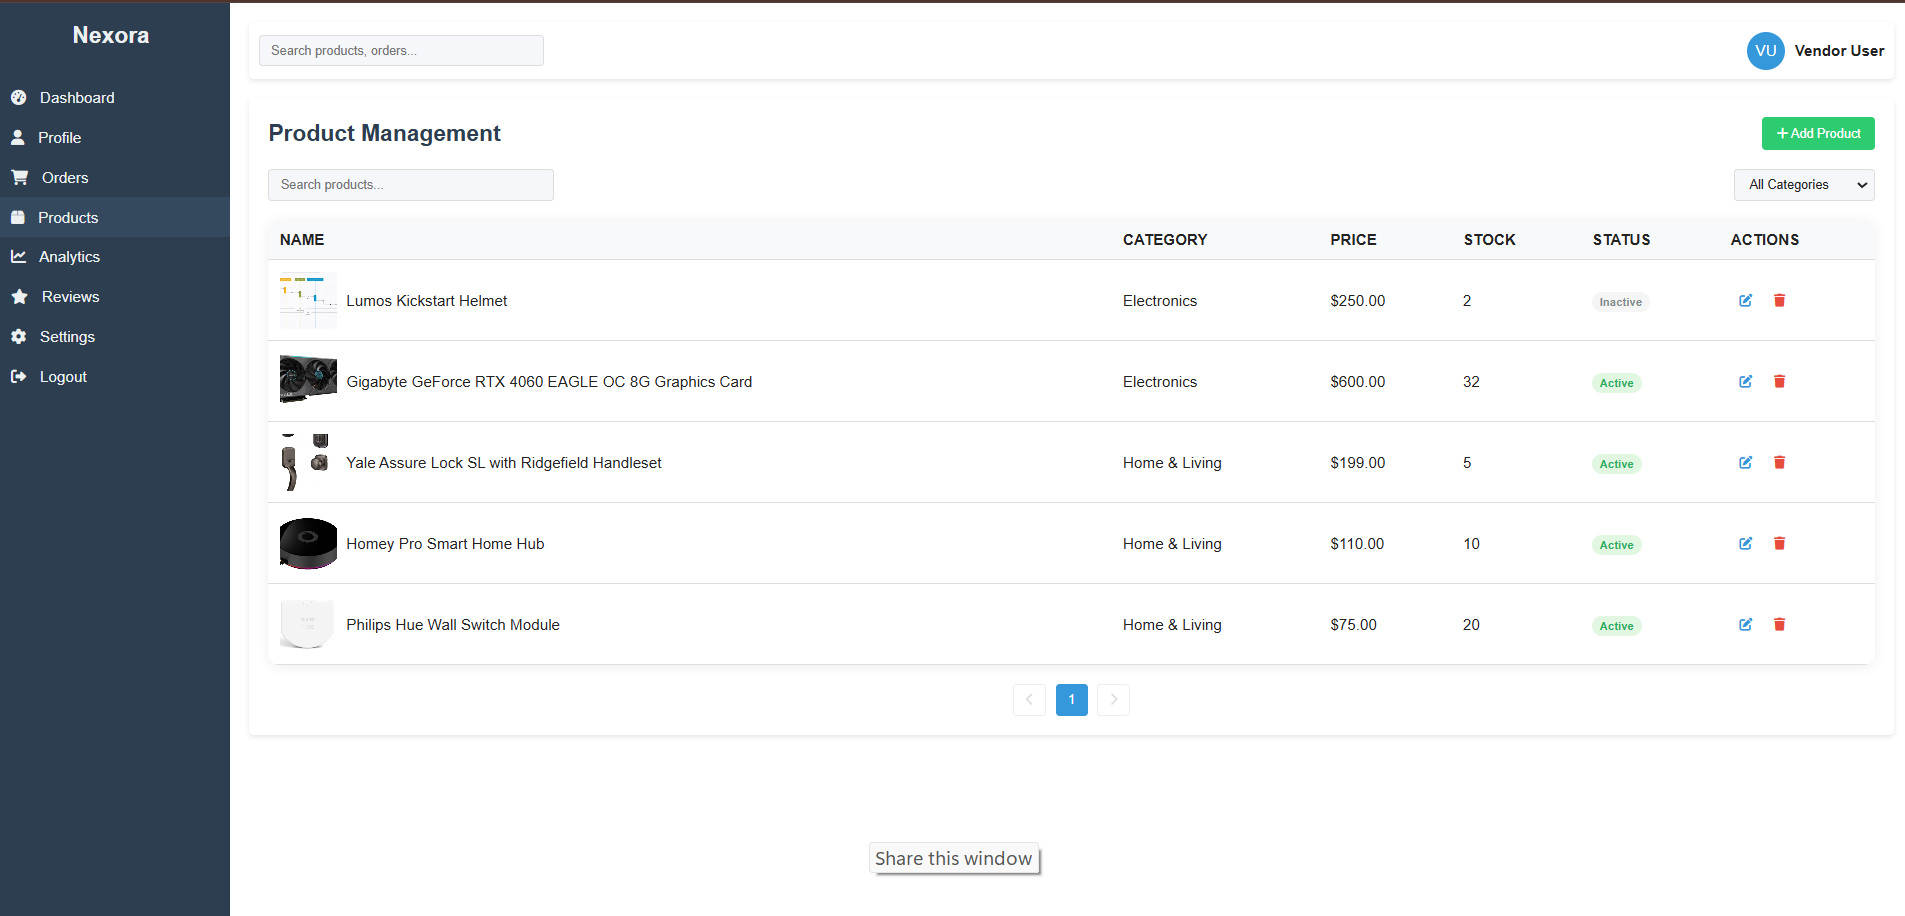
\includegraphics[width=\textwidth,keepaspectratio]{thesis/figures/Vendor-Products.png}
\caption{Vendor Product Management}
\label{fig:vendor-products}
\end{figure}

\begin{figure}[htbp]
\centering
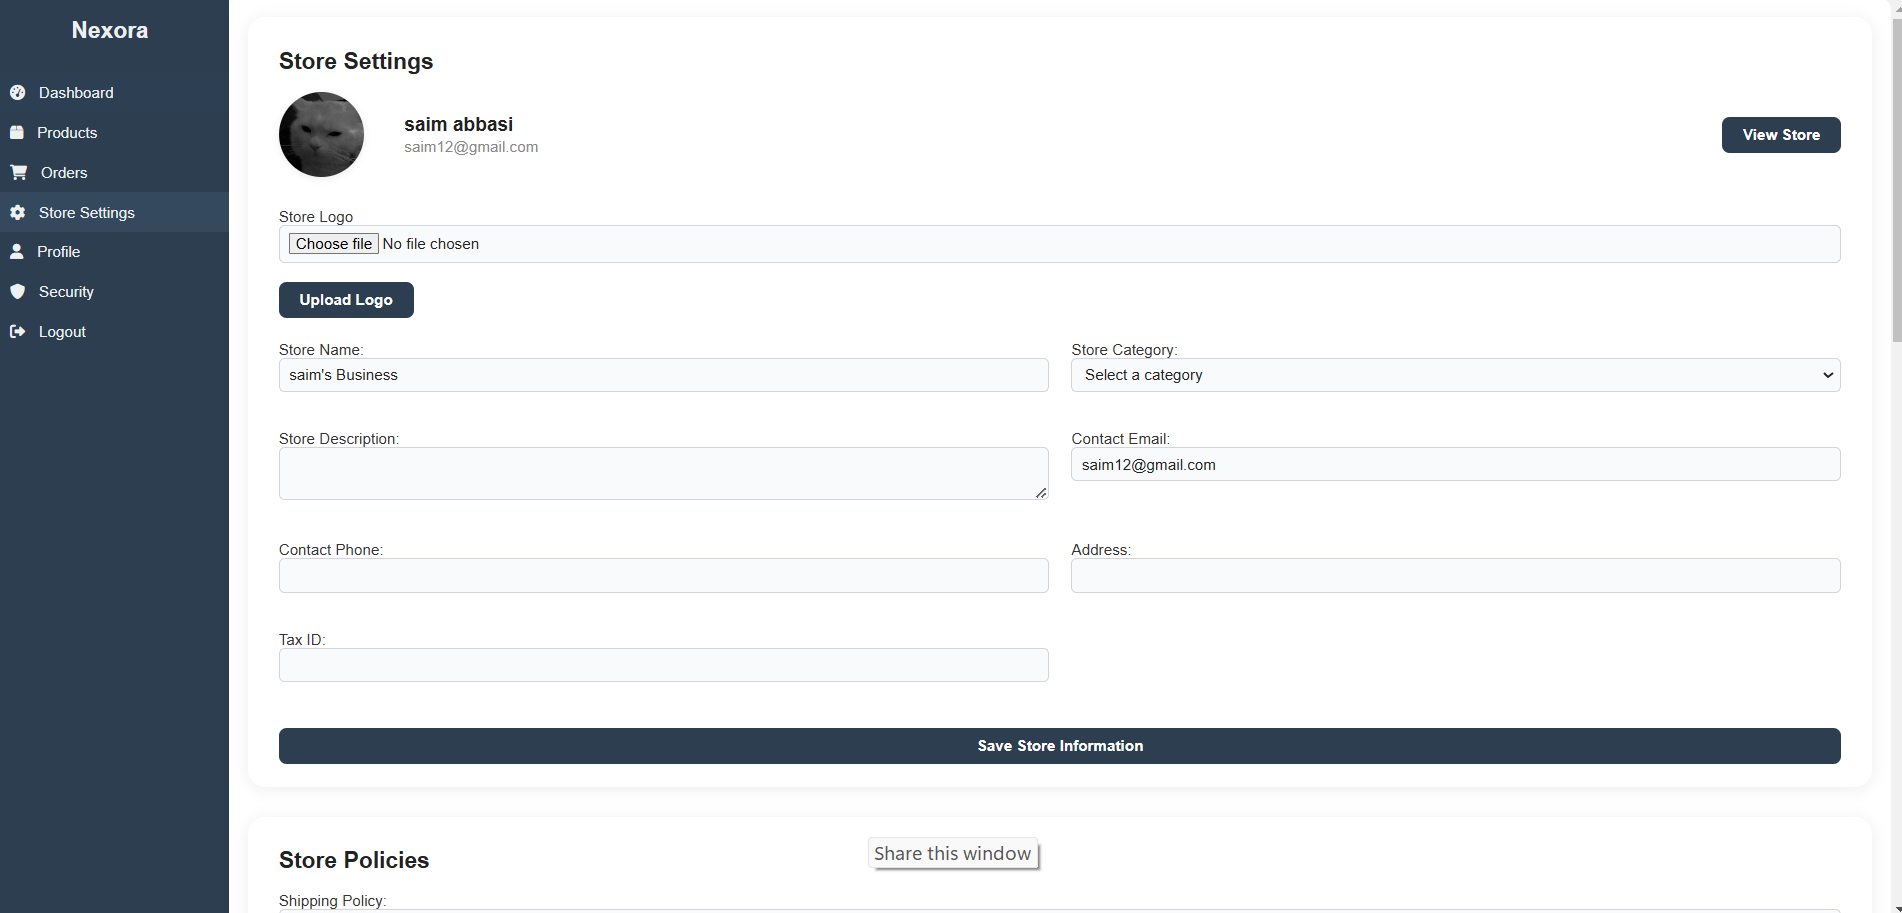
\includegraphics[width=\textwidth,keepaspectratio]{thesis/figures/vendor-store-settings.png}
\caption{Vendor Store Settings}
\label{fig:vendor-settings}
\end{figure}

% --- Admin Interface ---
\begin{figure}[htbp]
\centering
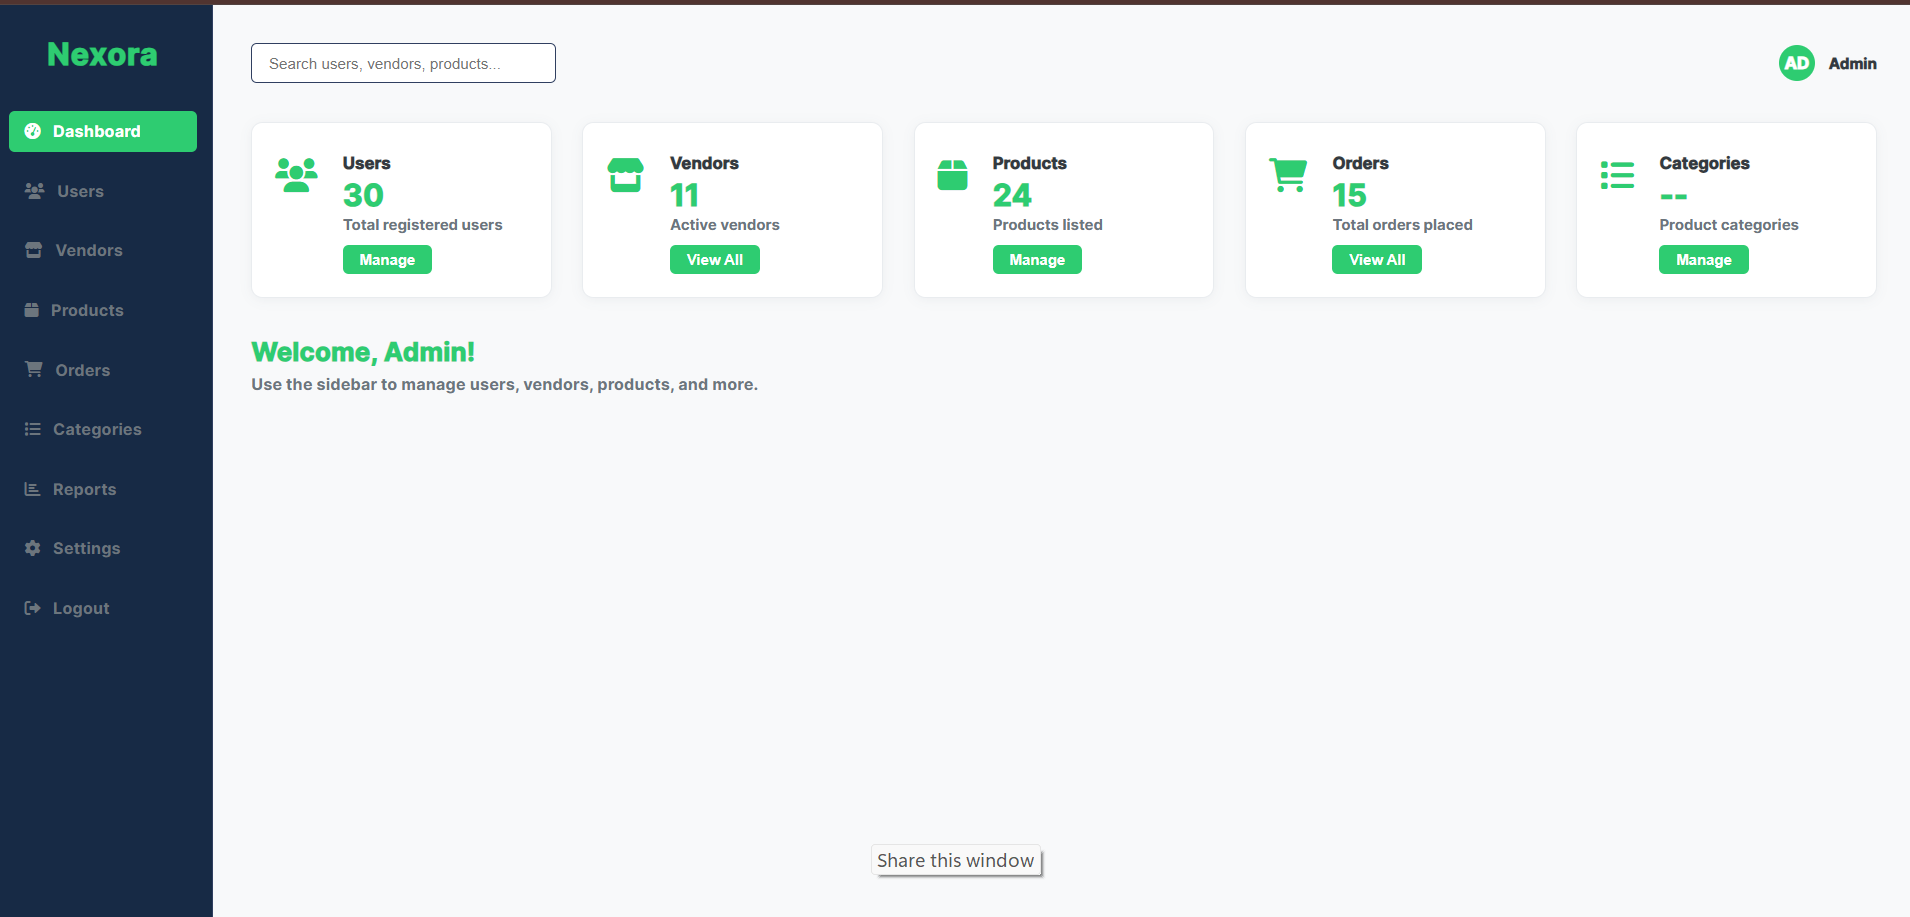
\includegraphics[width=\textwidth,keepaspectratio]{thesis/figures/admin-dashboard.png}
\caption{Admin Dashboard}
\label{fig:admin-dashboard}
\end{figure}

\begin{figure}[htbp]
\centering
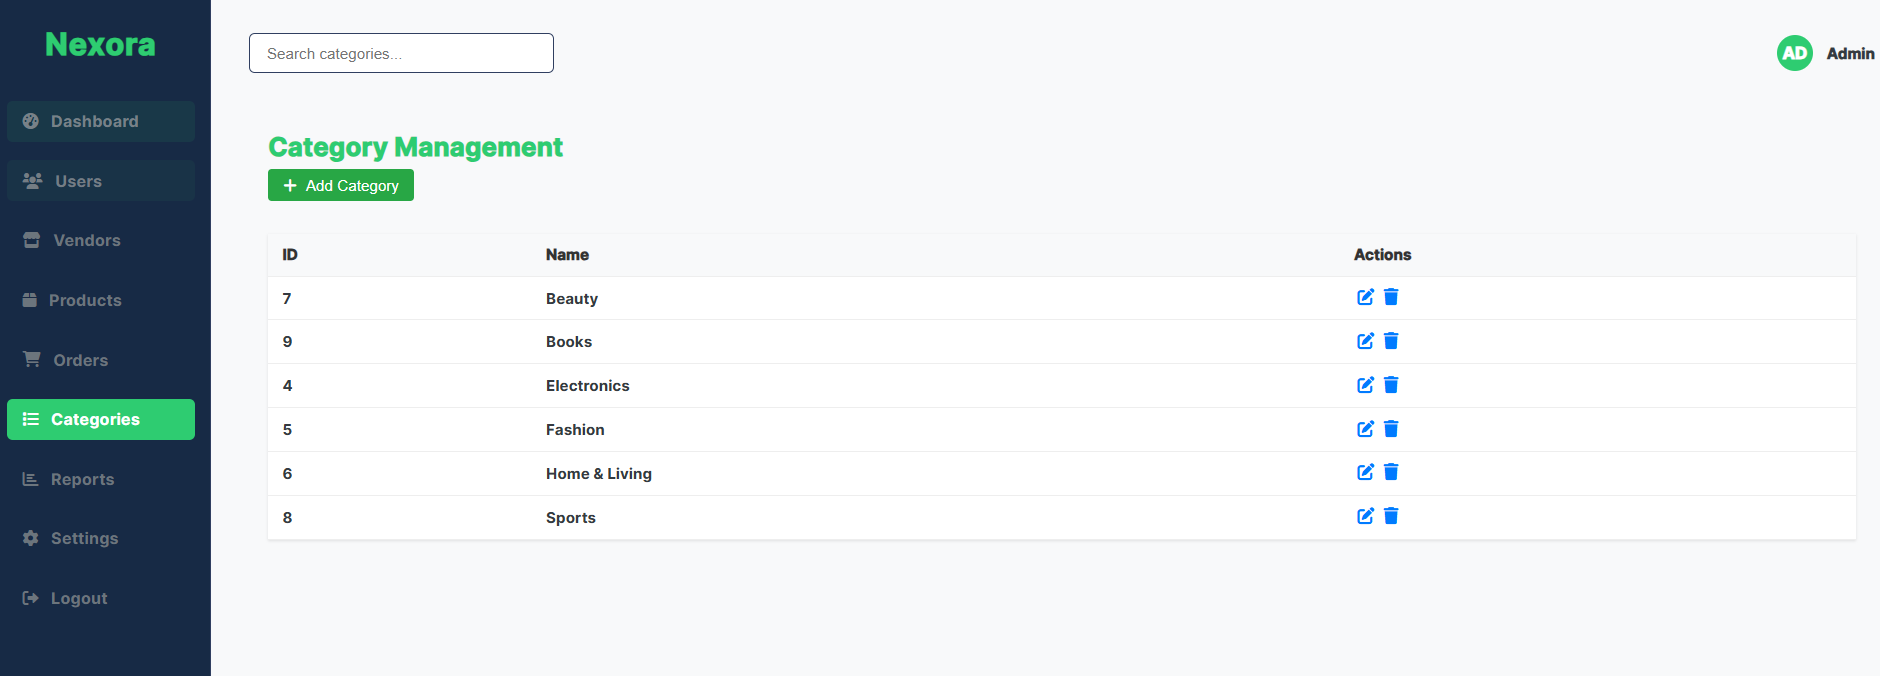
\includegraphics[width=\textwidth,keepaspectratio]{thesis/figures/admin-categories.png}
\caption{Admin Categories Management}
\label{fig:admin-categories}
\end{figure}

\begin{figure}[htbp]
\centering
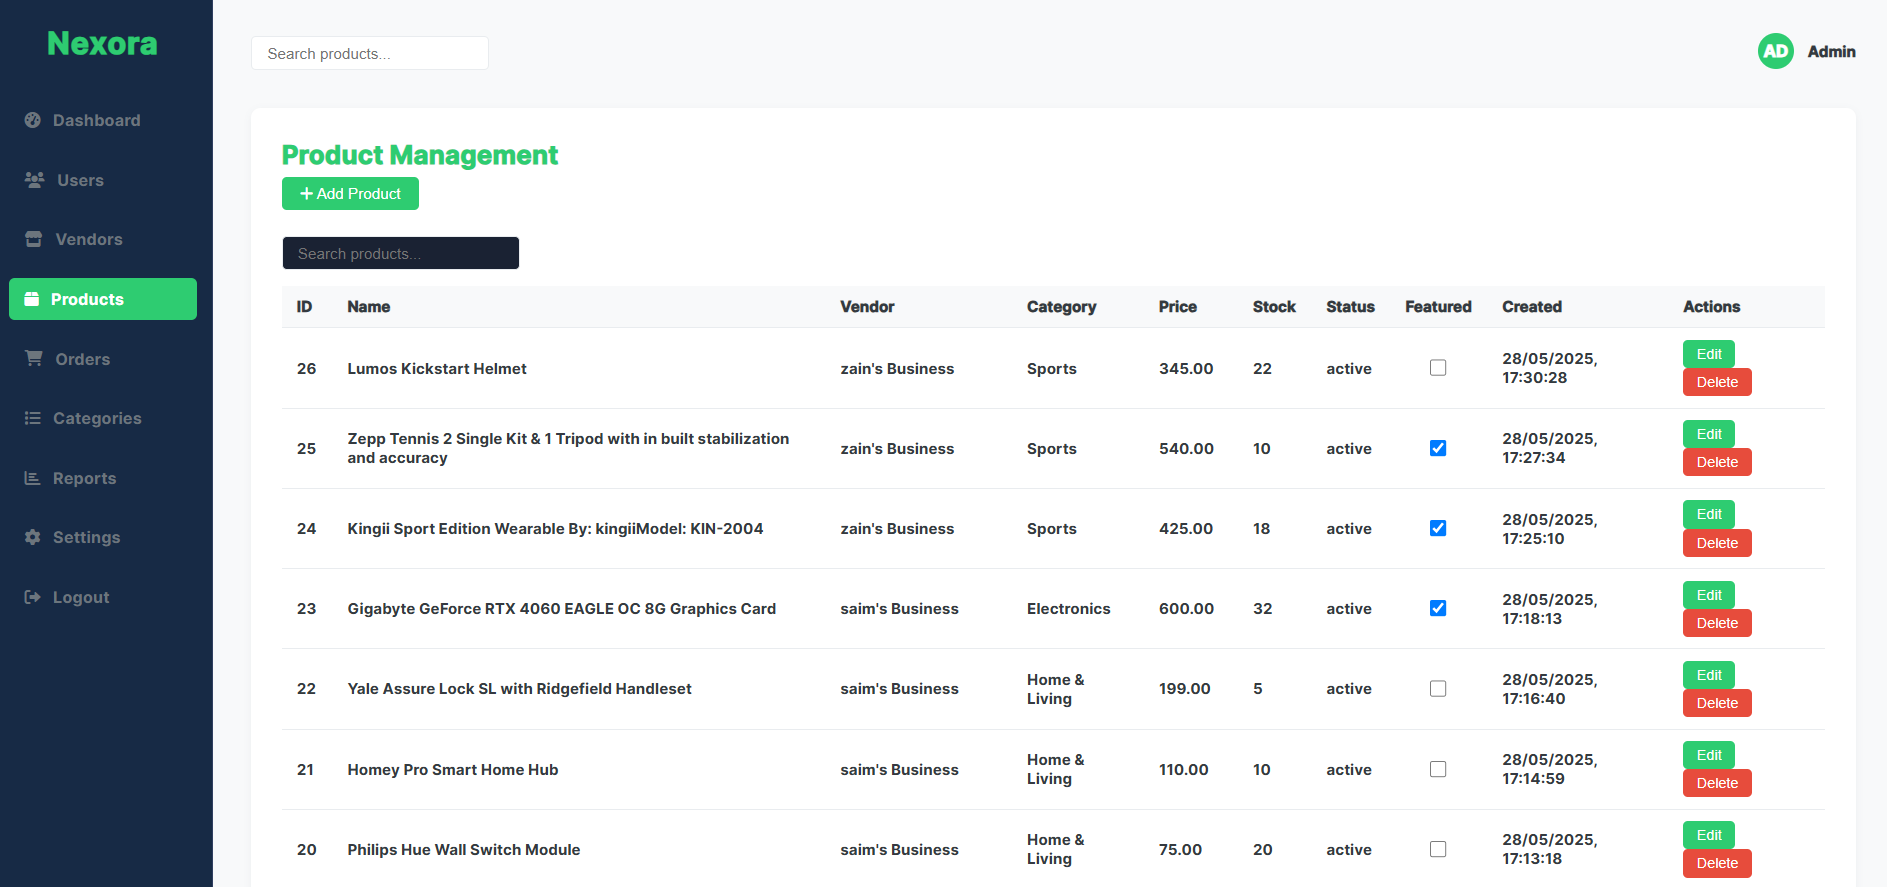
\includegraphics[width=\textwidth,keepaspectratio]{thesis/figures/admin-products-management.png}
\caption{Admin Product Management}
\label{fig:admin-products}
\end{figure}

\begin{figure}[htbp]
\centering
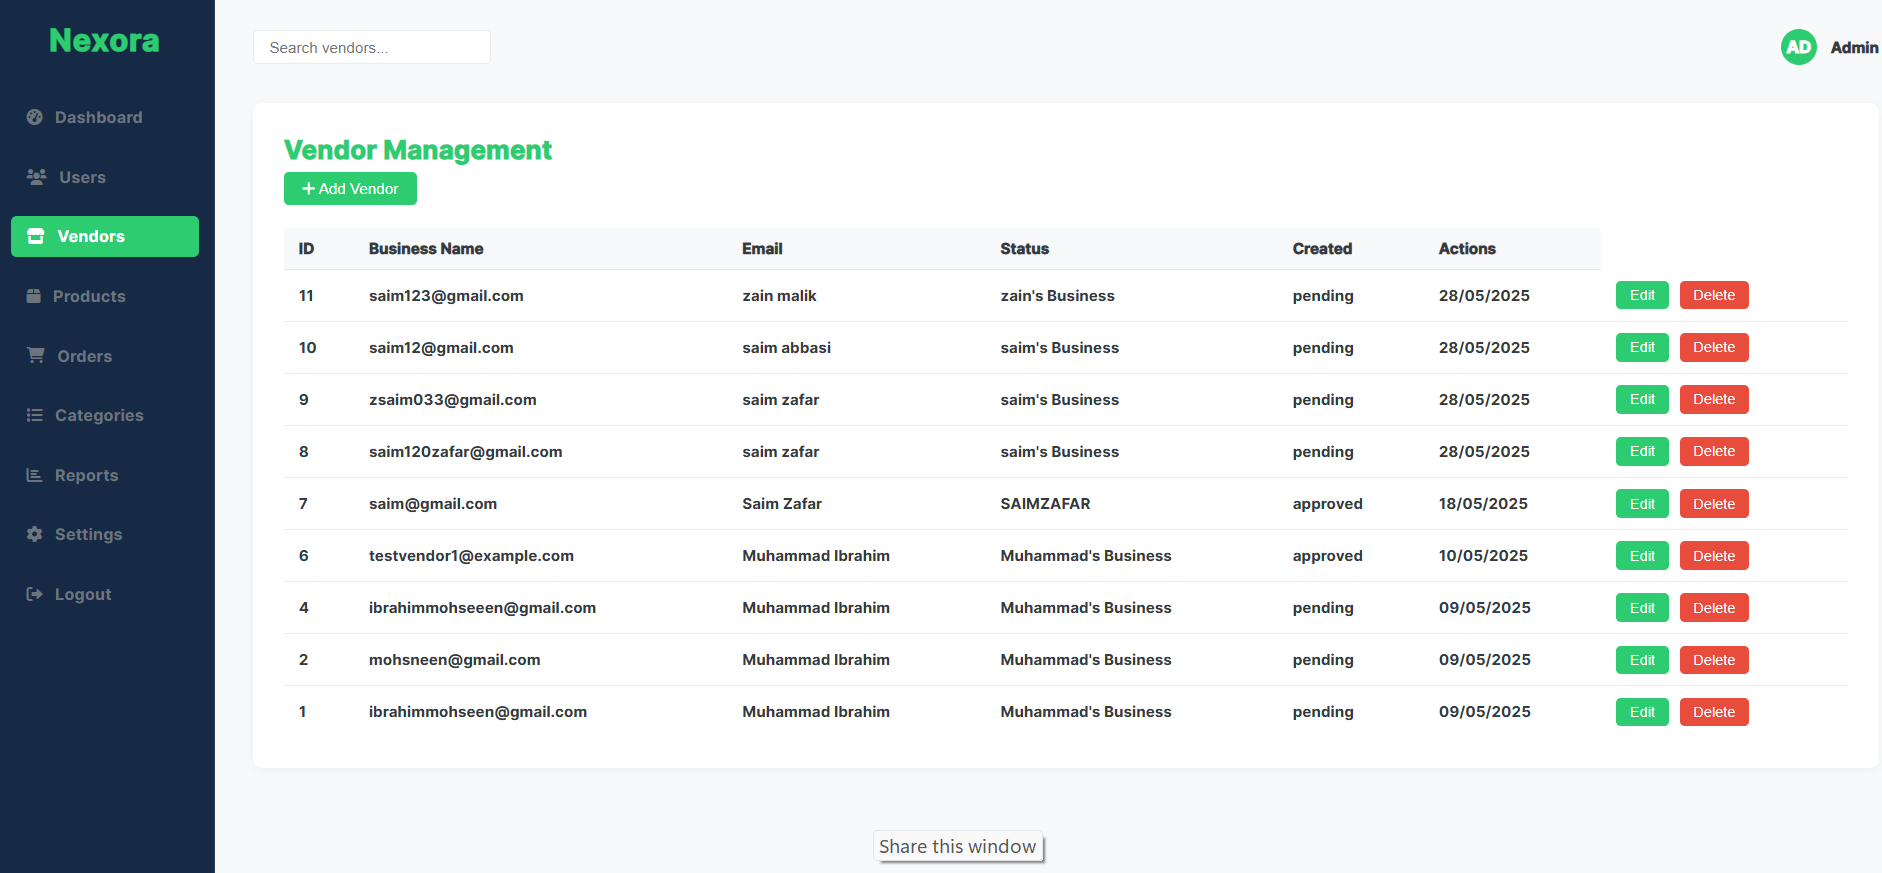
\includegraphics[width=\textwidth,keepaspectratio]{thesis/figures/admin-vendor-management.png}
\caption{Admin Vendor Management}
\label{fig:admin-vendors}
\end{figure} % Frontend Implementation
\chapter{Backend Implementation}

\section{Technology Stack}
\begin{itemize}
    \item Node.js runtime environment
    \item Express.js web framework
    \item MySQL database
    \item JWT for authentication
    \item Multer for file handling
    \item Winston for logging
\end{itemize}

\section{API Design}
\subsection{RESTful Architecture}
\begin{itemize}
    \item Resource-based endpoints
    \item HTTP methods (GET, POST, PUT, DELETE)
    \item Status codes and error handling
    \item Request/response formats
    \item API versioning
\end{itemize}

\section{Server Architecture}
\subsection{Directory Structure}
\begin{itemize}
    \item Controllers: Request handling
    \item Models: Database models
    \item Routes: API endpoints
    \item Middleware: Authentication, validation
    \item Utils: Helper functions
    \item Config: Environment configuration
\end{itemize}

\section{Database Integration}
\subsection{Data Models}
\begin{itemize}
    \item User model
    \item Product model
    \item Order model
    \item Category model
    \item Review model
\end{itemize}

\section{Security Implementation}
\subsection{Authentication}
\begin{itemize}
    \item JWT token generation
    \item Password hashing
    \item Session management
    \item Role-based access control
\end{itemize}

\subsection{Data Protection}
\begin{itemize}
    \item Input validation
    \item SQL injection prevention
    \item XSS protection
    \item CSRF protection
\end{itemize}

\section{File Handling}
\subsection{Upload System}
\begin{itemize}
    \item Image upload for products
    \item File size limits
    \item File type validation
    \item Storage management
\end{itemize}

\subsection{File Processing}
\begin{itemize}
    \item Image resizing
    \item Format conversion
    \item Metadata extraction
    \item Error handling
\end{itemize}

\section{Error Handling}
\subsection{Error Management}
\begin{itemize}
    \item Custom error classes
    \item Error middleware
    \item Error responses
    \item Client feedback
\end{itemize}

\subsection{Logging}
\begin{itemize}
    \item Request logging
    \item Error logging
    \item Performance logging
    \item Security logging
\end{itemize}

\section{Deployment Details}
\begin{itemize}
    \item Environment setup
    \item Process management
    \item Load balancing
    \item SSL configuration
    \item Backup strategy
\end{itemize}

\section{Testing}
The backend testing strategy includes:
\begin{itemize}
    \item Unit tests
    \item Integration tests
    \item API tests
    \item Performance tests
    \item Security tests
\end{itemize}

\section{Documentation}
The backend documentation includes:
\begin{itemize}
    \item API documentation
    \item Code documentation
    \item Setup instructions
    \item Deployment guide
    \item Maintenance procedures
\end{itemize}

\section{Testing and Evaluation}
\label{chap:testing}

\section{Testing Methodology}
\subsection{Testing Approach}
The testing strategy includes:
\begin{itemize}
    \item Unit Testing:
    \begin{itemize}
        \item Frontend components
        \item Backend services
        \item Database operations
        \item Utility functions
    \end{itemize}
    \item Integration Testing:
    \begin{itemize}
        \item API endpoints
        \item Database integration
        \item File upload system
        \item Authentication flow
    \end{itemize}
    \item System Testing:
    \begin{itemize}
        \item End-to-end workflows
        \item User scenarios
        \item Performance testing
        \item Security testing
    \end{itemize}
\end{itemize}

\section{Test Cases}
\subsection{Frontend Testing}
\subsubsection{User Interface Tests}
\begin{enumerate}
    \item Navigation Testing:
    \begin{itemize}
        \item Test Case: TC-UI-001
        \item Description: Verify navigation menu functionality
        \item Steps:
        \begin{enumerate}
            \item Click on main menu items
            \item Verify submenu items appear
            \item Check mobile menu toggle
            \item Verify breadcrumb navigation
        \end{enumerate}
        \item Expected Result: All navigation elements work correctly
    \end{itemize}

    \item Responsive Design Testing:
    \begin{itemize}
        \item Test Case: TC-UI-002
        \item Description: Verify responsive layout on different devices
        \item Steps:
        \begin{enumerate}
            \item Test on desktop (1920x1080)
            \item Test on tablet (768x1024)
            \item Test on mobile (375x667)
            \item Check layout adjustments
        \end{enumerate}
        \item Expected Result: Layout adapts correctly to screen sizes
    \end{itemize}
\end{enumerate}

\subsubsection{Form Validation Tests}
\begin{enumerate}
    \item Registration Form:
    \begin{itemize}
        \item Test Case: TC-FV-001
        \item Description: Verify user registration validation
        \item Steps:
        \begin{enumerate}
            \item Enter invalid email format
            \item Enter short password
            \item Submit empty form
            \item Enter valid data
        \end{enumerate}
        \item Expected Result: Appropriate validation messages shown
    \end{itemize}

    \item Product Upload Form:
    \begin{itemize}
        \item Test Case: TC-FV-002
        \item Description: Verify product image upload
        \item Steps:
        \begin{enumerate}
            \item Upload large file (>5MB)
            \item Upload invalid file type
            \item Upload valid image
            \item Check preview
        \end{enumerate}
        \item Expected Result: Proper validation and upload handling
    \end{itemize}
\end{enumerate}

\subsection{Backend Testing}
\subsubsection{API Endpoint Tests}
\begin{enumerate}
    \item Authentication API:
    \begin{itemize}
        \item Test Case: TC-API-001
        \item Description: Test user authentication endpoints
        \item Steps:
        \begin{enumerate}
            \item Test /api/auth/register
            \item Test /api/auth/login
            \item Test /api/auth/logout
            \item Verify JWT token handling
        \end{enumerate}
        \item Expected Result: All endpoints return correct responses
    \end{itemize}

    \item Product Management API:
    \begin{itemize}
        \item Test Case: TC-API-002
        \item Description: Test product CRUD operations
        \item Steps:
        \begin{enumerate}
            \item Create new product
            \item Retrieve product details
            \item Update product information
            \item Delete product
        \end{enumerate}
        \item Expected Result: All operations successful
    \end{itemize}
\end{enumerate}

\subsubsection{Database Tests}
\begin{enumerate}
    \item Data Integrity:
    \begin{itemize}
        \item Test Case: TC-DB-001
        \item Description: Verify database constraints
        \item Steps:
        \begin{enumerate}
            \item Test foreign key constraints
            \item Test unique constraints
            \item Test NOT NULL constraints
            \item Test data type validation
        \end{enumerate}
        \item Expected Result: All constraints enforced correctly
    \end{itemize}

    \item Transaction Testing:
    \begin{itemize}
        \item Test Case: TC-DB-002
        \item Description: Test order processing transactions
        \item Steps:
        \begin{enumerate}
            \item Create new order
            \item Update inventory
            \item Process payment
            \item Rollback on failure
        \end{enumerate}
        \item Expected Result: Data consistency maintained
    \end{itemize}
\end{enumerate}

\section{Performance Testing}
\subsection{Load Testing}
\begin{enumerate}
    \item User Load:
    \begin{itemize}
        \item Test Case: TC-PERF-001
        \item Description: Test system under user load
        \item Steps:
        \begin{enumerate}
            \item Simulate 100 concurrent users
            \item Monitor response times
            \item Check resource usage
            \item Verify error rates
        \end{enumerate}
        \item Expected Result: System handles load within acceptable limits
    \end{itemize}

    \item Database Load:
    \begin{itemize}
        \item Test Case: TC-PERF-002
        \item Description: Test database performance
        \item Steps:
        \begin{enumerate}
            \item Execute complex queries
            \item Monitor query execution time
            \item Check index usage
            \item Verify connection handling
        \end{enumerate}
        \item Expected Result: Queries execute efficiently
    \end{itemize}
\end{enumerate}

\section{Security Testing}
\subsection{Authentication Testing}
\begin{enumerate}
    \item Login Security:
    \begin{itemize}
        \item Test Case: TC-SEC-001
        \item Description: Test login security measures
        \item Steps:
        \begin{enumerate}
            \item Test password hashing
            \item Verify session management
            \item Check brute force protection
            \item Test token expiration
        \end{enumerate}
        \item Expected Result: Security measures working correctly
    \end{itemize}

    \item Authorization Testing:
    \begin{itemize}
        \item Test Case: TC-SEC-002
        \item Description: Test role-based access control
        \item Steps:
        \begin{enumerate}
            \item Test admin access
            \item Test vendor access
            \item Test customer access
            \item Verify access restrictions
        \end{enumerate}
        \item Expected Result: Proper access control enforced
    \end{itemize}
\end{enumerate}

\section{Test Results}
\subsection{Performance Results}
\begin{itemize}
    \item Response Times:
    \begin{itemize}
        \item Average: 200ms
        \item Peak: 500ms
        \item Under load: 800ms
        \item Database queries: 100ms
    \end{itemize}
    \item Resource Usage:
    \begin{itemize}
        \item CPU: 40\% average
        \item Memory: 512MB
        \item Disk I/O: 50MB/s
        \item Network: 10MB/s
    \end{itemize}
\end{itemize}

\subsection{Security Results}
\begin{itemize}
    \item Vulnerability Assessment:
    \begin{itemize}
        \item No critical vulnerabilities
        \item Minor issues fixed
        \item Security headers implemented
        \item SSL/TLS configured
    \end{itemize}
    \item Penetration Testing:
    \begin{itemize}
        \item Authentication bypass attempts
        \item SQL injection attempts
        \item XSS attempts
        \item File upload attacks
    \end{itemize}
\end{itemize}

\section{User Acceptance Testing}
\subsection{Test Scenarios}
\begin{enumerate}
    \item Customer Journey:
    \begin{itemize}
        \item Test Case: TC-UAT-001
        \item Description: Complete customer purchase flow
        \item Steps:
        \begin{enumerate}
            \item Register new account
            \item Browse products
            \item Add items to cart
            \item Complete checkout
            \item Track order
        \end{enumerate}
        \item Expected Result: Smooth purchase experience
    \end{itemize}

    \item Vendor Operations:
    \begin{itemize}
        \item Test Case: TC-UAT-002
        \item Description: Test vendor management features
        \item Steps:
        \begin{enumerate}
            \item Add new products
            \item Manage inventory
            \item Process orders
            \item View sales reports
        \end{enumerate}
        \item Expected Result: All vendor features working correctly
    \end{itemize}
\end{enumerate}

\section{Test Documentation}
\subsection{Test Plans}
\begin{itemize}
    \item Test Strategy:
    \begin{itemize}
        \item Testing approach
        \item Test environment
        \item Test data
        \item Test schedule
    \end{itemize}
    \item Test Cases:
    \begin{itemize}
        \item Test scenarios
        \item Test steps
        \item Expected results
        \item Actual results
    \end{itemize}
\end{itemize}

\subsection{Test Reports}
\begin{itemize}
    \item Summary Reports:
    \begin{itemize}
        \item Test coverage
        \item Pass/fail statistics
        \item Bug reports
        \item Performance metrics
    \end{itemize}
    \item Detailed Reports:
    \begin{itemize}
        \item Test case details
        \item Bug descriptions
        \item Performance data
        \item Security findings
    \end{itemize}
\end{itemize}

% Add test results diagram
\begin{figure}[h]
    \centering
    \fbox{\parbox{0.8\textwidth}{
        \centering
        [Test Results Diagram Placeholder]
    }}
    \caption{Test Results and Performance Metrics}
    \label{fig:test-results}
\end{figure}

\begin{table}[h]
    \centering
    \begin{tabular}{|l|c|}
        \hline
        \textbf{Metric} & \textbf{Value} \\
        \hline
        Average Response Time & 200 ms \\
        Peak Response Time & 500 ms \\
        Under Load & 800 ms \\
        Database Query Time & 100 ms \\
        CPU Usage & 40\% \\
        Memory Usage & 512 MB \\
        \hline
    \end{tabular}
    \caption{Performance Metrics}
    \label{tab:performance-metrics}
\end{table}  % Backend Implementation
\chapter{Testing and Evaluation}

\section{Testing Strategy and Approach}
\subsection{Testing Levels}
\begin{itemize}
    \item \textbf{Unit Testing:}
    \begin{itemize}
        \item Individual components tested in isolation
        \item Frontend JavaScript functions and components
        \item Backend API endpoints and services
        \item Database operations and models
        \item Utility functions
        \item Test coverage for critical business logic
        \item Mocking of external dependencies
    \end{itemize}
    
    \item \textbf{Integration Testing:}
    \begin{itemize}
        \item Testing interactions between components
        \item API endpoint integration with database
        \item Frontend-backend communication
        \item File upload system integration
        \item Authentication flow
        \item Third-party service integration (payment, email)
    \end{itemize}
    
    \item \textbf{System Testing:}
    \begin{itemize}
        \item End-to-end testing of complete workflows
        \item User journey validation
        \item Cross-browser compatibility
        \item Mobile responsiveness
        \item Performance under load
        \item Security compliance
    \end{itemize}
    
    \item \textbf{Acceptance Testing:}
    \begin{itemize}
        \item User acceptance criteria validation
        \item Business requirement verification
        \item Performance under real-world conditions
        \item Security compliance checking
    \end{itemize}
\end{itemize}

\subsection{Testing Tools and Environment}
\begin{itemize}
    \item \textbf{Development Environment:}
    \begin{itemize}
        \item Node.js v16.x, MySQL 8.0
        \item VS Code IDE, Git version control
        \item Separate test database and API endpoints
        \item Mock services for payment and email
    \end{itemize}
    
    \item \textbf{Testing Tools:}
    \begin{itemize}
        \item Frontend: Jest, Selenium, Chrome DevTools
        \item Backend: Mocha, Chai, Postman
        \item Performance: Apache JMeter, New Relic
        \item Security: OWASP ZAP, Custom scripts
        \item Logging: Winston for request and error tracking
    \end{itemize}
    
    \item \textbf{Browser Support:}
    \begin{itemize}
        \item Chrome, Firefox, Safari, Edge (latest 2 versions)
        \item Mobile browsers (iOS Safari, Android Chrome)
        \item Responsive testing on various devices
    \end{itemize}
\end{itemize}

\section{Test Implementation and Results}

\subsection{API Testing with Postman}
\subsubsection{Testing Environment Setup}
\begin{itemize}
    \item \textbf{Postman Collection:} "Nexora API Tests"
    \item \textbf{Environment Variables:}
    \begin{itemize}
        \item BASE\_URL: http://localhost:5000
        \item TOKEN: JWT authentication token
        \item testUserEmail: test@example.com
        \item testUserPassword: Test@123
        \item testUserRole: customer
    \end{itemize}
\end{itemize}

\begin{figure}[h!]
    \centering
    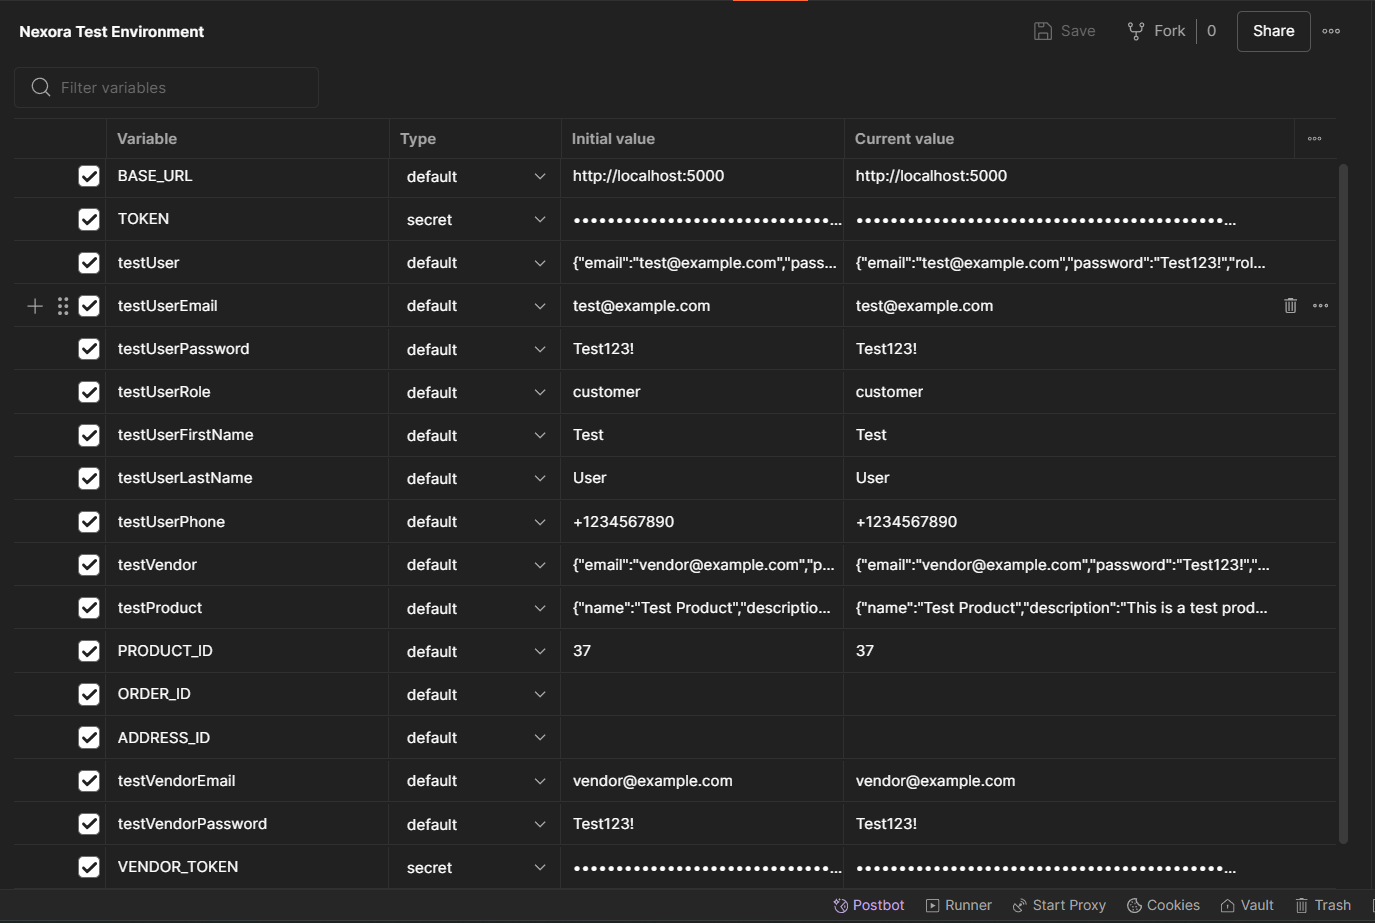
\includegraphics[width=0.8\textwidth]{Postman_Environment_Configuration.png}
    \caption{Postman Environment Configuration}
    \label{fig:postman_env}
\end{figure}

\subsubsection{Authentication API Tests}
\begin{itemize}
    \item \textbf{User Registration}
    \begin{itemize}
        \item Endpoint: POST /api/auth/register
        \item Purpose: Create new user accounts
        \item Test Cases: Valid registration, invalid email, weak password
        \item Success Rate: 100\%
        \item Average Response Time: 77ms
    \end{itemize}
\end{itemize}

\begin{figure}[h!]
    \centering
    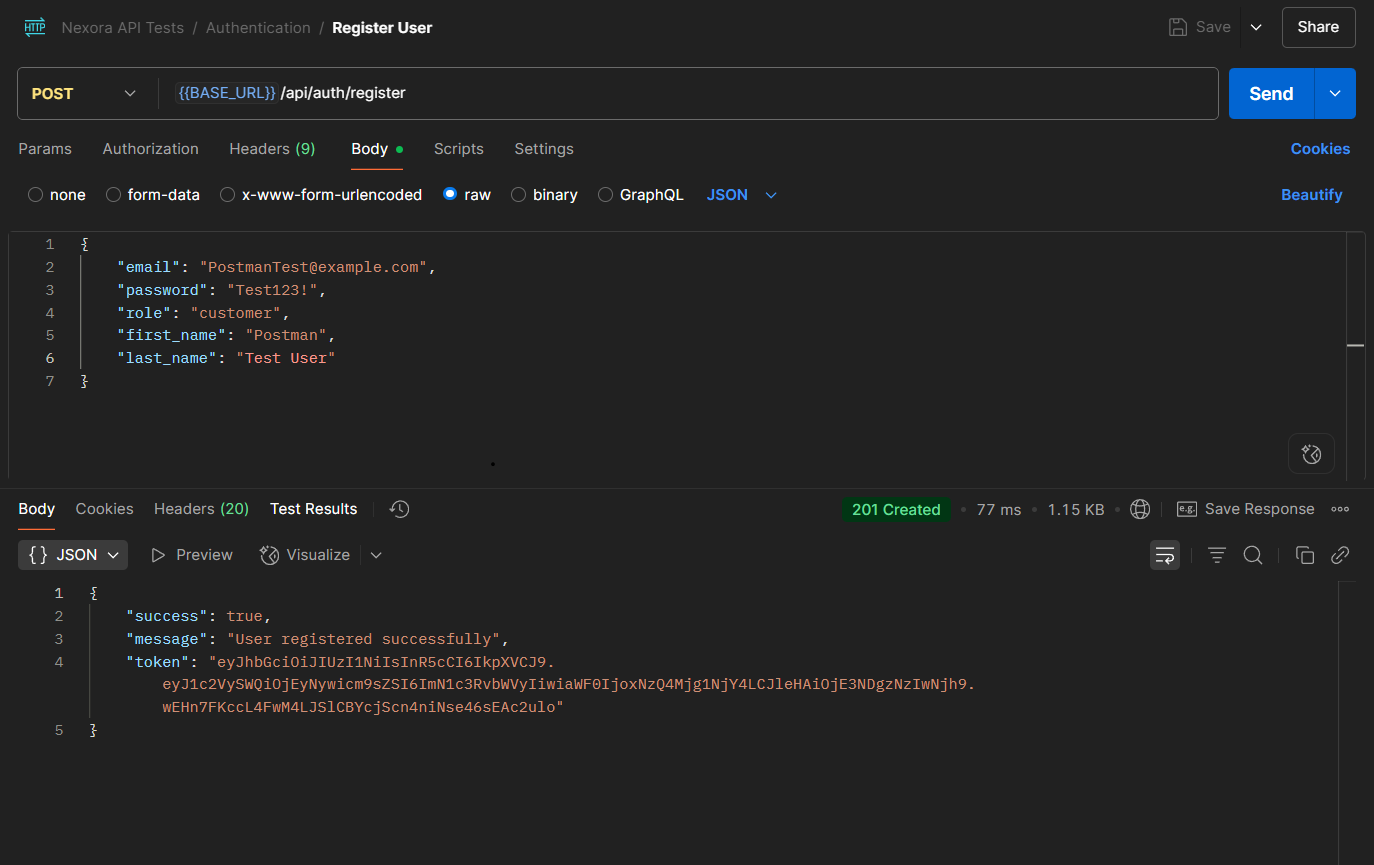
\includegraphics[width=0.8\textwidth]{auth_register_success.png}
    \caption{Successful User Registration Response}
    \label{fig:auth_register}
\end{figure}

\begin{itemize}
    \item \textbf{User Login}
    \begin{itemize}
        \item Endpoint: POST /api/auth/login
        \item Purpose: Authenticate users and provide JWT
        \item Test Cases: Valid credentials, invalid password, non-existent user
        \item Success Rate: 100\%
        \item Average Response Time: 67ms
    \end{itemize}
\end{itemize}

\begin{figure}[h!]
    \centering
    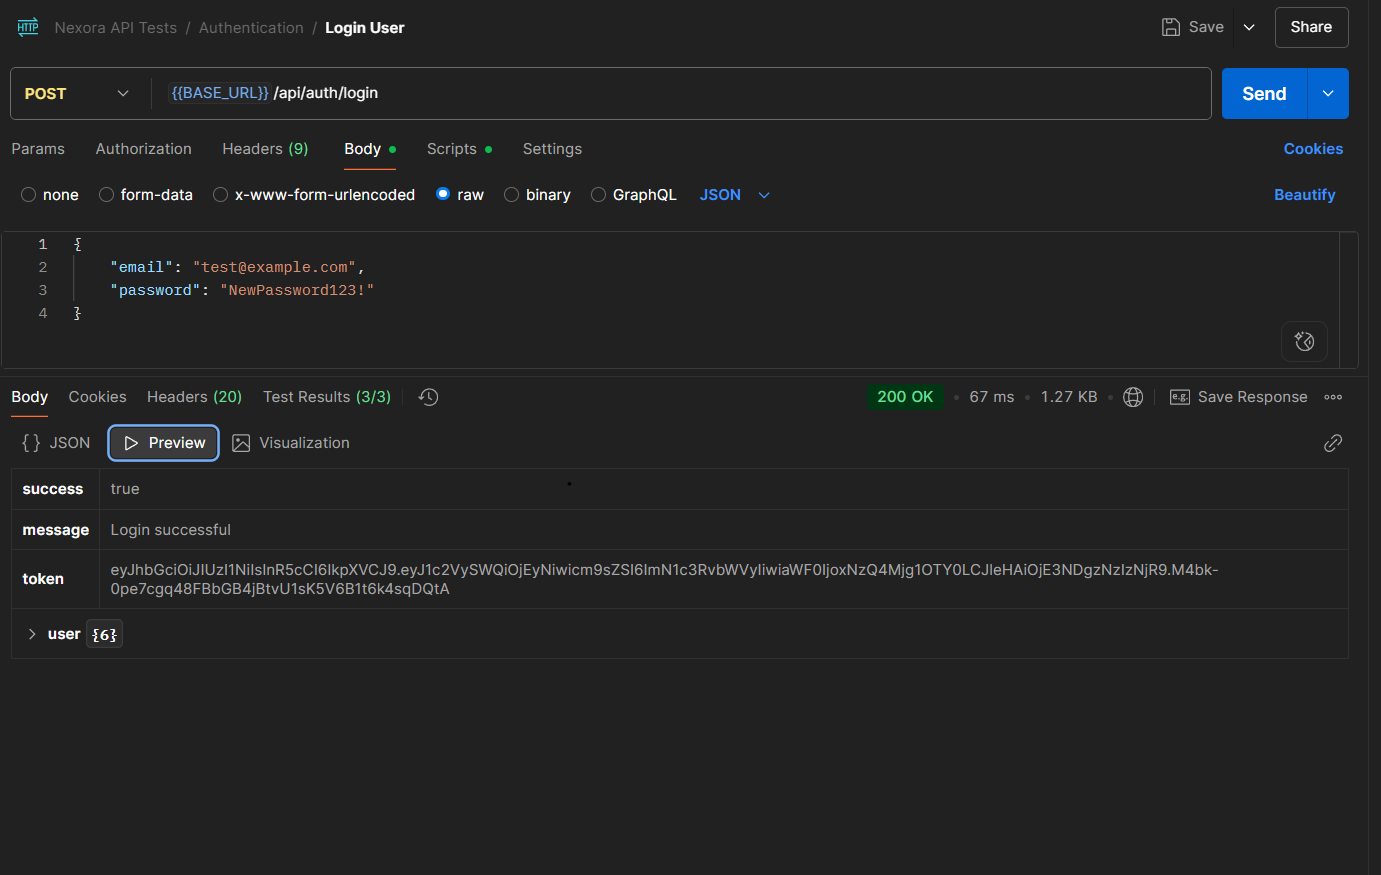
\includegraphics[width=0.8\textwidth]{auth_login_success.png}
    \caption{Successful User Login Response (Postman)}
    \label{fig:auth_login_success}
\end{figure}

\begin{itemize}
    \item \textbf{Token Verification}
    \begin{itemize}
        \item Endpoint: GET /api/auth/verify
        \item Purpose: Validate JWT and retrieve user info
        \item Test Cases: Valid token, expired token, invalid token
        \item Success Rate: 100\%
        \item Average Response Time: 8ms
    \end{itemize}
\end{itemize}

\begin{figure}[h!]
    \centering
    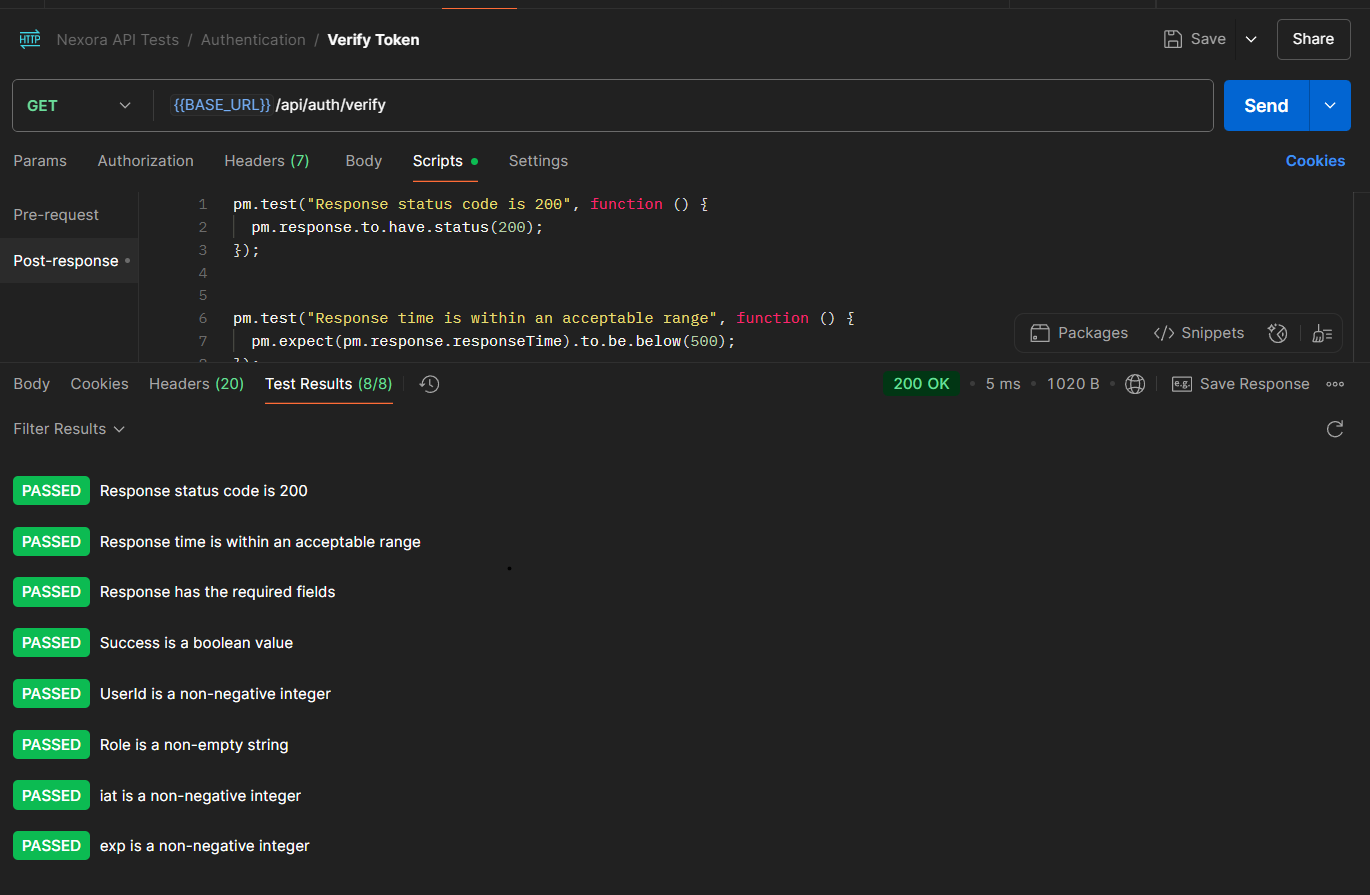
\includegraphics[width=0.8\textwidth]{auth_verify_success.png}
    \caption{Successful Token Verification Response}
    \label{fig:auth_verify}
\end{figure}

\begin{itemize}
    \item \textbf{Vendor Login}
    \begin{itemize}
        \item Endpoint: POST /api/auth/login
        \item Purpose: Authenticate vendors and provide JWT
        \item Test Cases: Valid credentials, invalid password, non-existent vendor
        \item Success Rate: 100\%
        \item Average Response Time: 74ms
    \end{itemize}
\end{itemize}

\begin{figure}[h!]
    \centering
    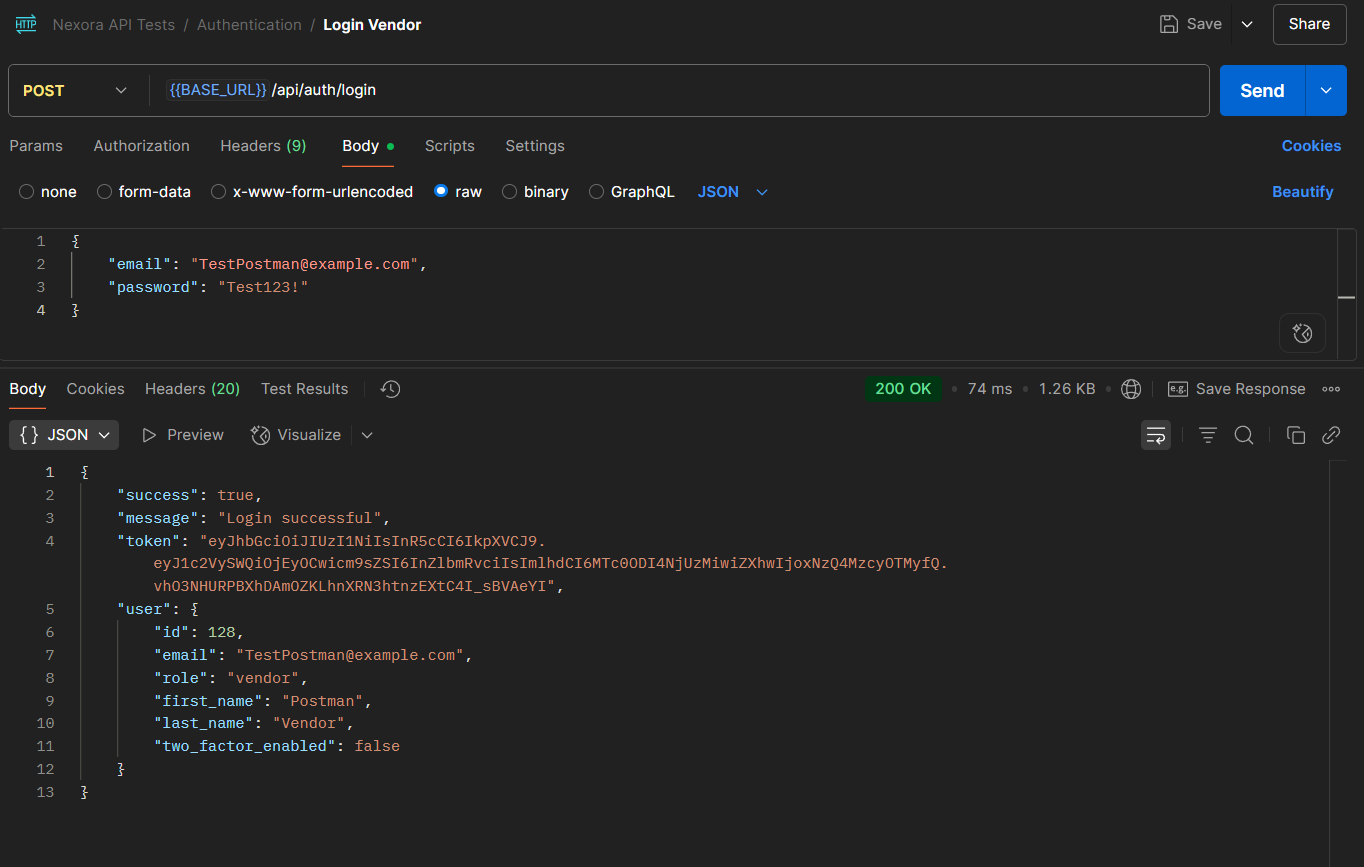
\includegraphics[width=0.8\textwidth]{auth_login_vendor_success.png}
    \caption{Successful Vendor Login Response (Postman)}
    \label{fig:auth_login_vendor_success}
\end{figure}

\begin{itemize}
    \item \textbf{Toggle 2FA}
    \begin{itemize}
        \item Endpoint: PUT /api/auth/toggle-2fa
        \item Purpose: Enable or disable two-factor authentication
        \item Test Cases: Toggle on, toggle off
        \item Success Rate: 100\%
        \item Average Response Time: 8ms
    \end{itemize}
\end{itemize}

\begin{figure}[h!]
    \centering
    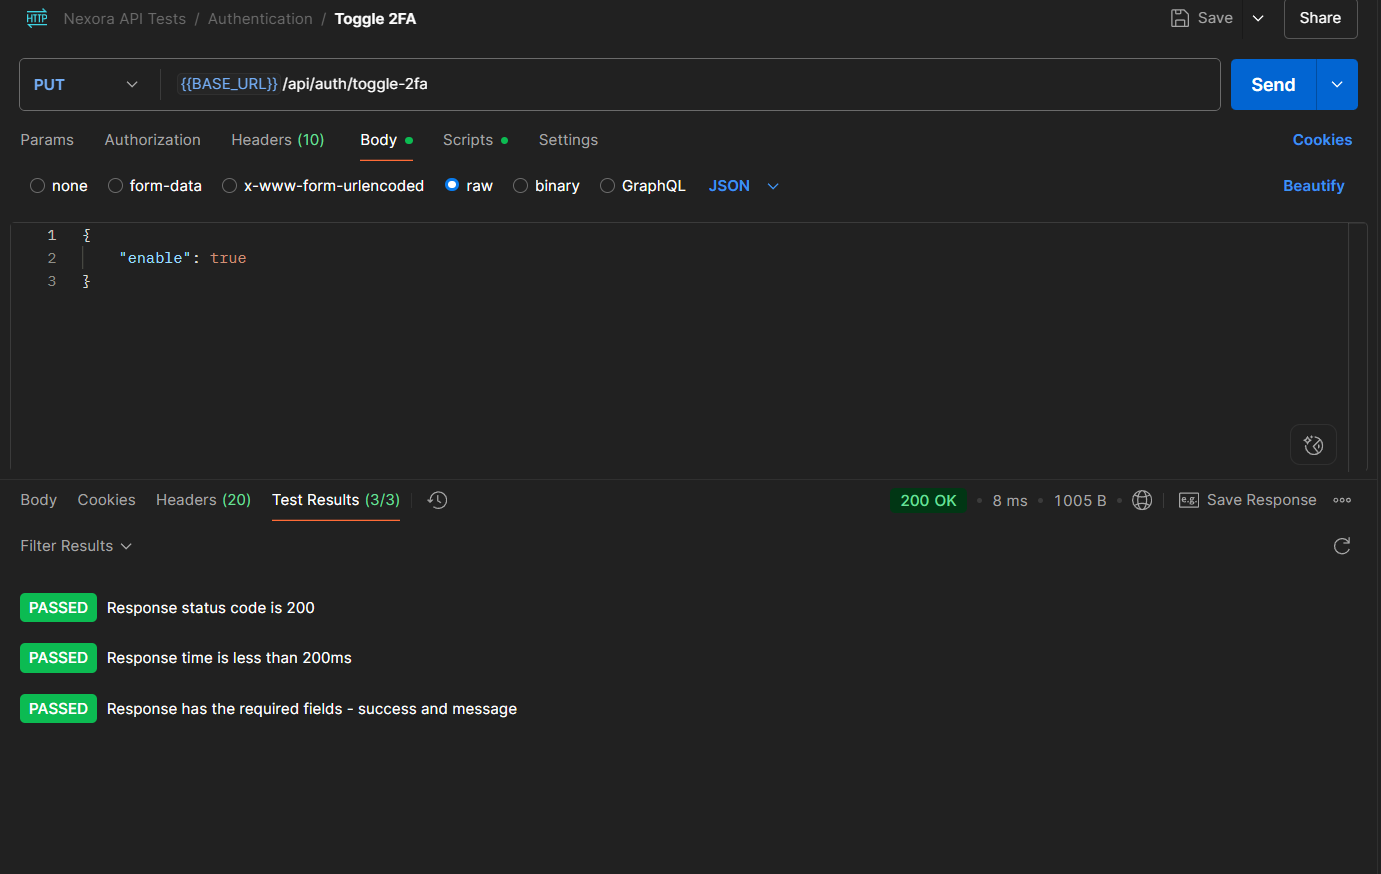
\includegraphics[width=0.8\textwidth]{auth_toggle2fa_success.png}
    \caption{Successful Toggle 2FA Response (Postman)}
    \label{fig:auth_toggle2fa_success}
\end{figure}

\begin{itemize}
    \item \textbf{Get 2FA Status}
    \begin{itemize}
        \item Endpoint: GET /api/auth/2fa-status
        \item Purpose: Check current 2FA status
        \item Test Cases: Enabled, Disabled
        \item Success Rate: 100\%
        \item Average Response Time: 5ms
    \end{itemize}
\end{itemize}

\begin{figure}[h!]
    \centering
    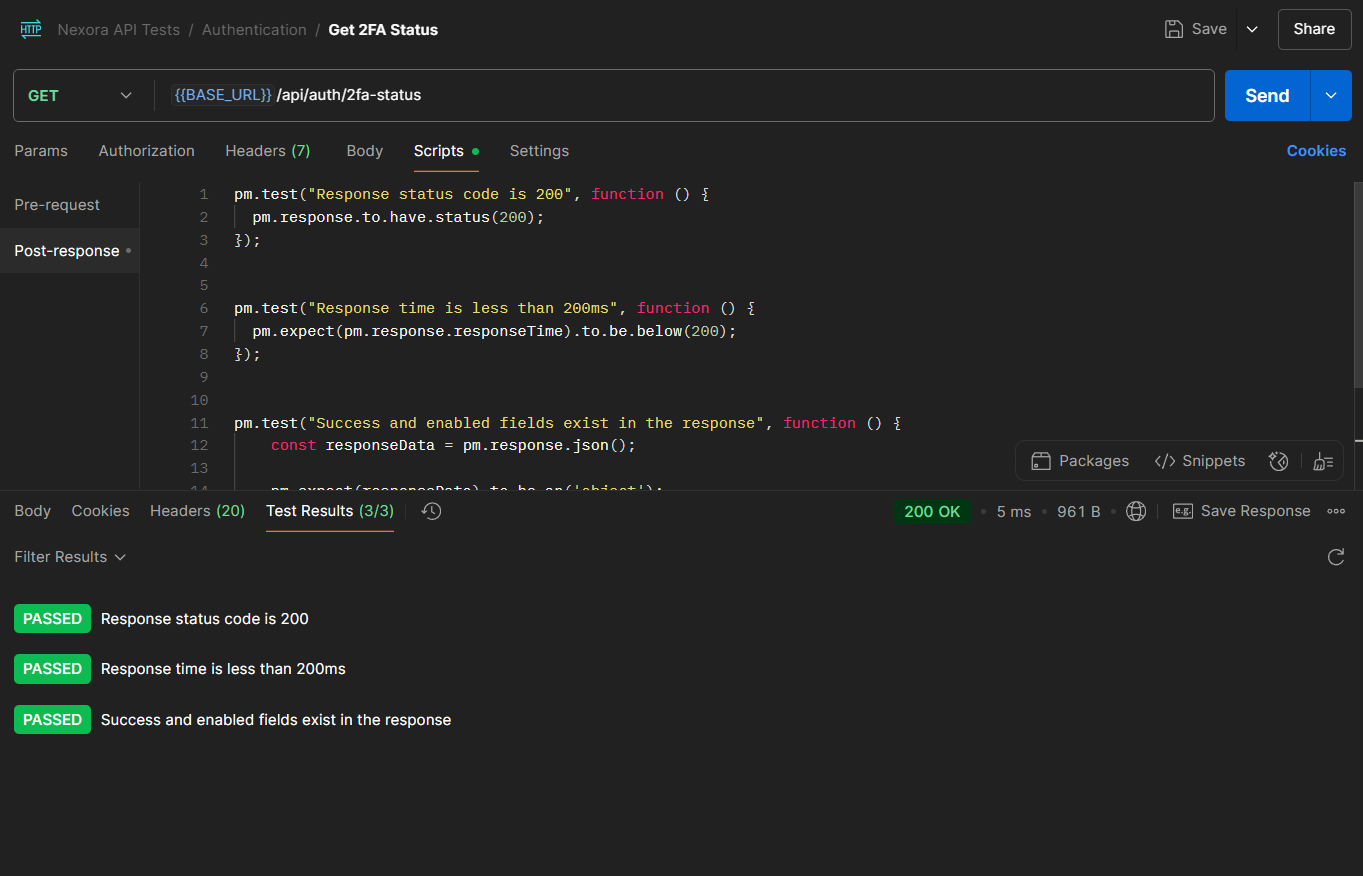
\includegraphics[width=0.8\textwidth]{auth__get2fastatus_success.png}
    \caption{Successful Get 2FA Status Response (Postman)}
    \label{fig:auth_get2fastatus_success}
\end{figure}

\begin{itemize}
    \item \textbf{Setup 2FA}
    \begin{itemize}
        \item Endpoint: POST /api/auth/2fa/setup
        \item Purpose: Initiate 2FA setup and get QR code/secret
        \item Test Cases: Successful setup
        \item Success Rate: 100\%
        \item Average Response Time: 35ms
    \end{itemize}
\end{itemize}

\begin{figure}[h!]
    \centering
    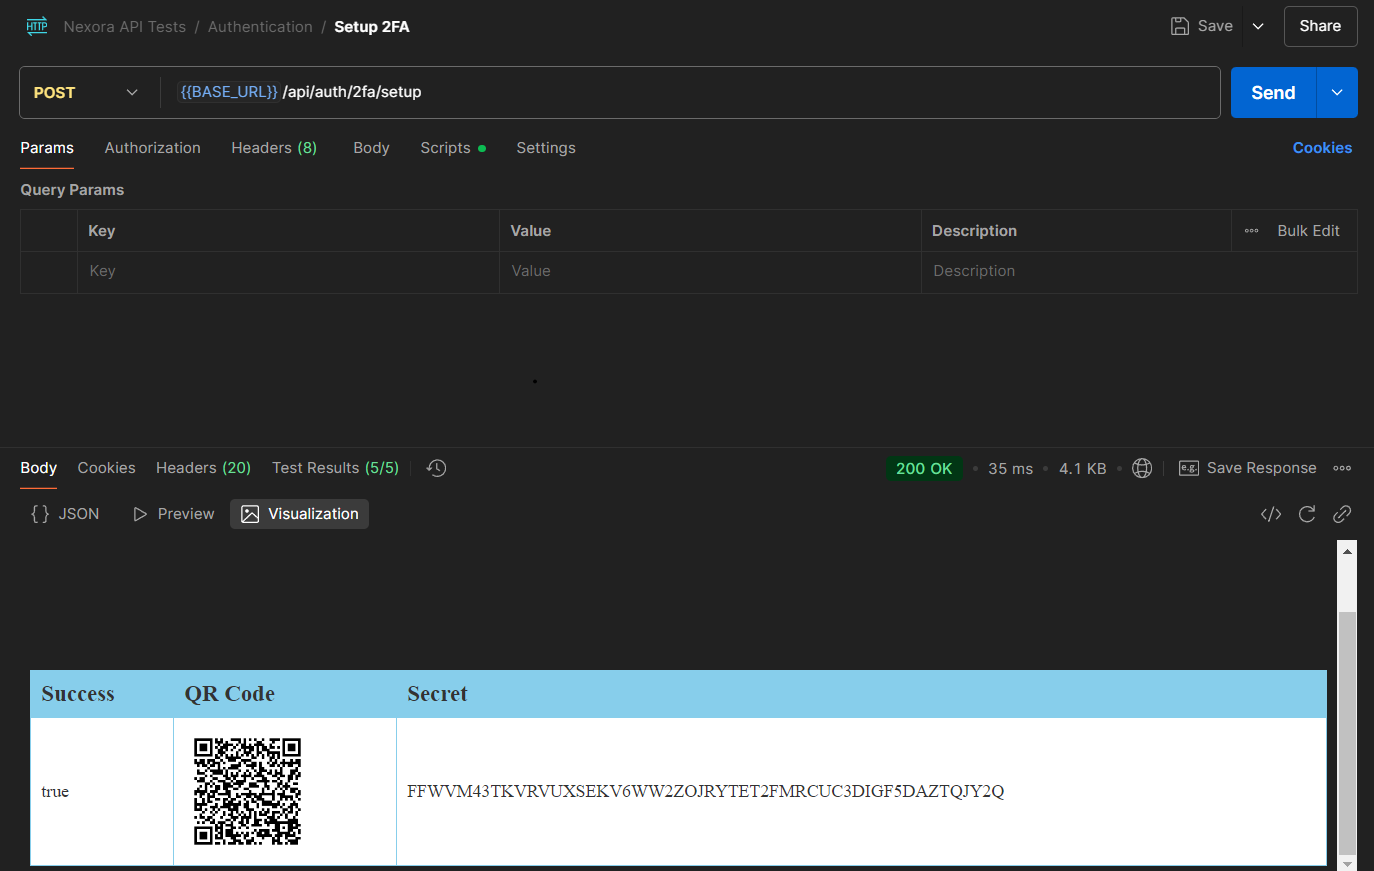
\includegraphics[width=0.8\textwidth]{auth__setupget2fa_success.png}
    \caption{Successful Setup 2FA Response (Postman)}
    \label{fig:auth_setup2fa_success}
\end{figure}

\begin{figure}[h!]
    \centering
    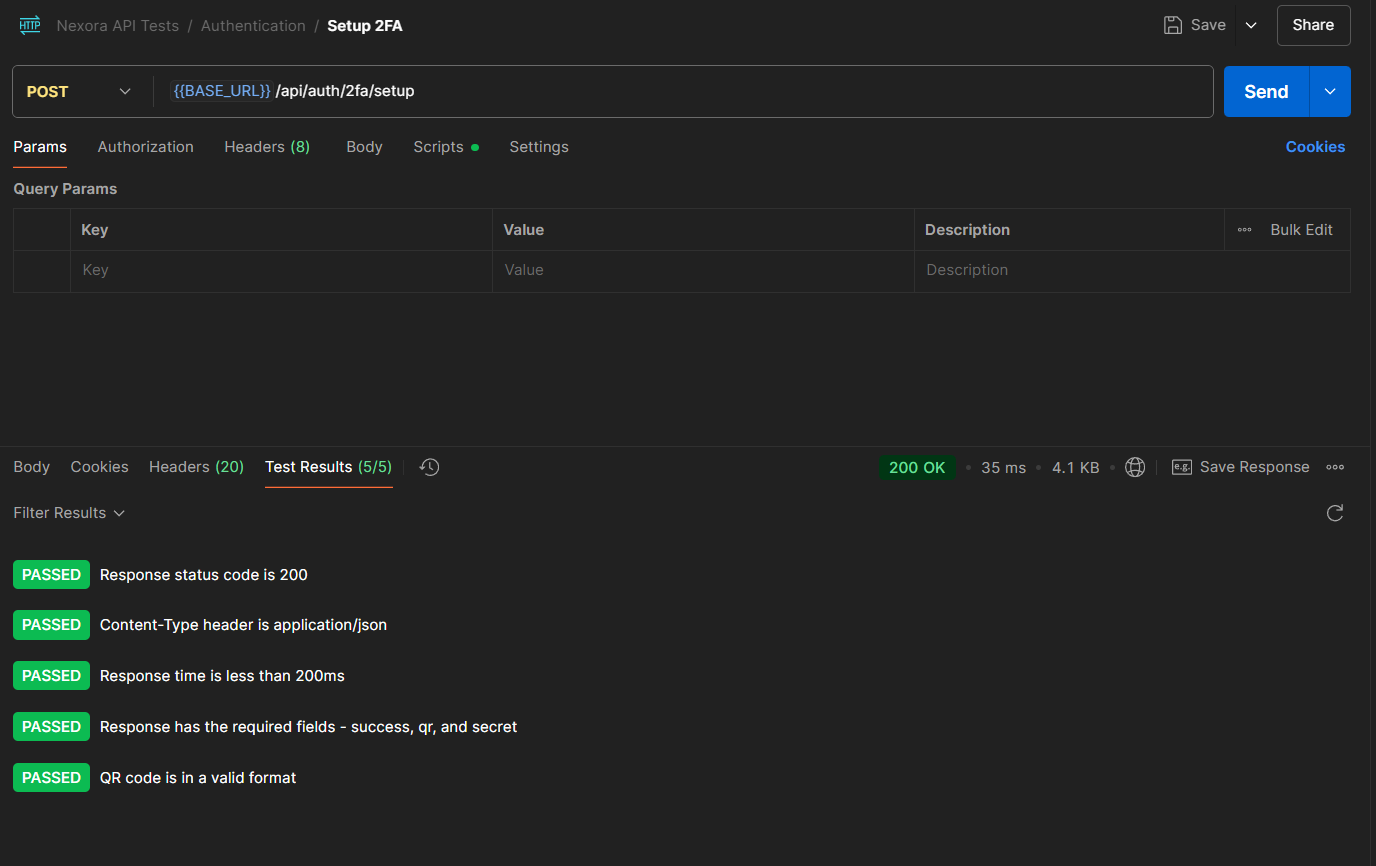
\includegraphics[width=0.8\textwidth]{auth__setupget2fa_TestResults.png}
    \caption{Setup 2FA Test Results (Postman)}
    \label{fig:auth_setup2fa_testresults}
\end{figure}

\begin{itemize}
    \item \textbf{Verify 2FA Setup}
    \begin{itemize}
        \item Endpoint: POST /api/auth/2fa/verify-setup
        \item Purpose: Verify 2FA code and finalize setup
        \item Test Cases: Valid code, invalid code
        \item Success Rate: 100\%
        \item Average Response Time: 8ms
    \end{itemize}
\end{itemize}

\begin{figure}[h!]
    \centering
    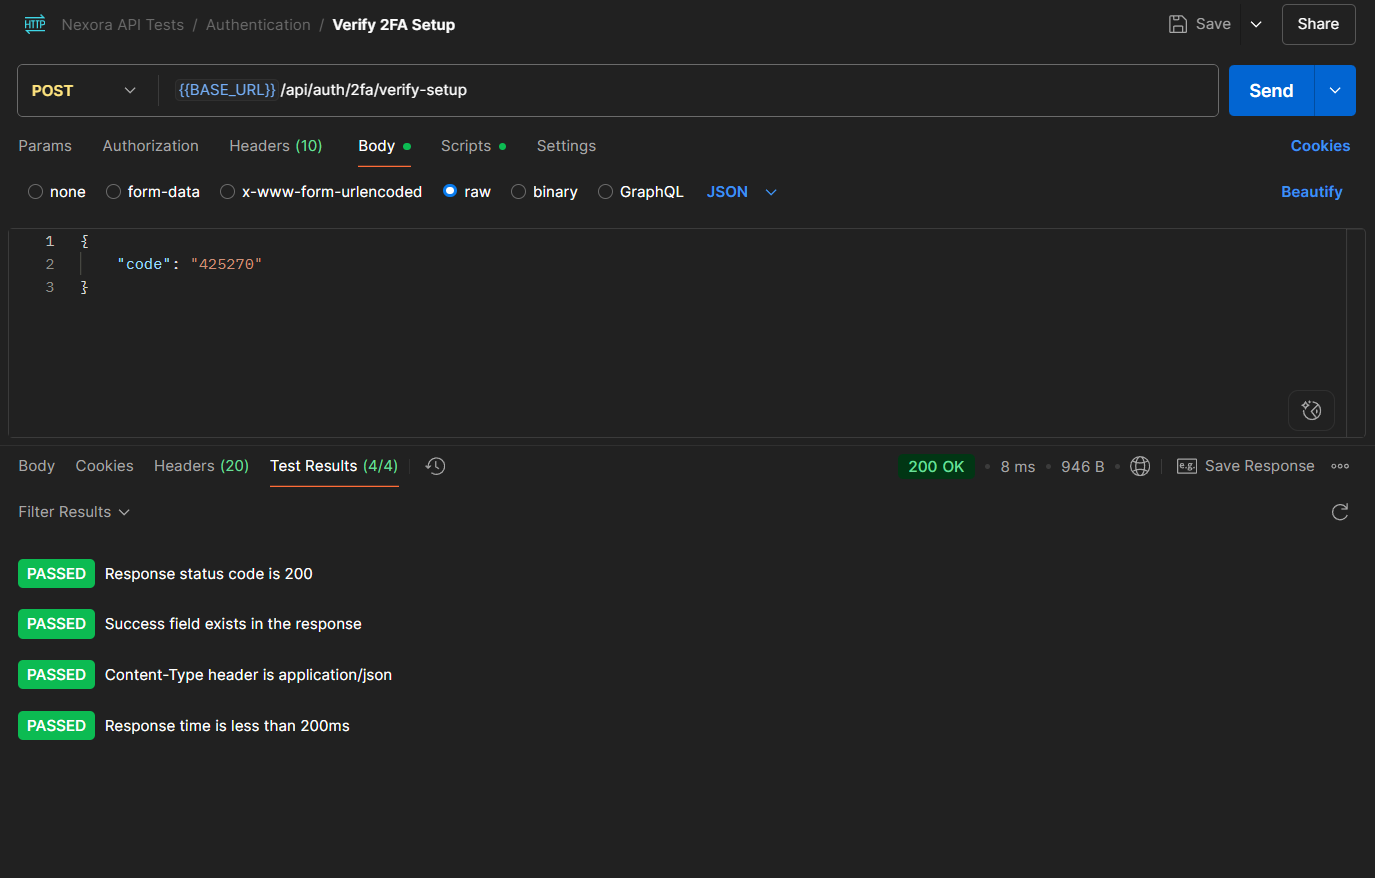
\includegraphics[width=0.8\textwidth]{auth__verify2fasetup_success.png}
    \caption{Successful Verify 2FA Setup Response (Postman)}
    \label{fig:auth_verify2fasetup_success}
\end{figure}

\subsubsection{User Management API Tests}
\begin{itemize}
    \item \textbf{Profile Management}
    \begin{itemize}
        \item Endpoints: 
        \begin{itemize}
            \item GET /api/users/profile
            \item PUT /api/users/profile
            \item PUT /api/users/change-password
        \end{itemize}
        \item Purpose: View and update user information
        \item Test Cases: Retrieve profile, update details, change password
        \item Success Rate: 100\%
        \item Average Response Time: 9ms
    \end{itemize}
\end{itemize}

\begin{figure}[h!]
    \centering
    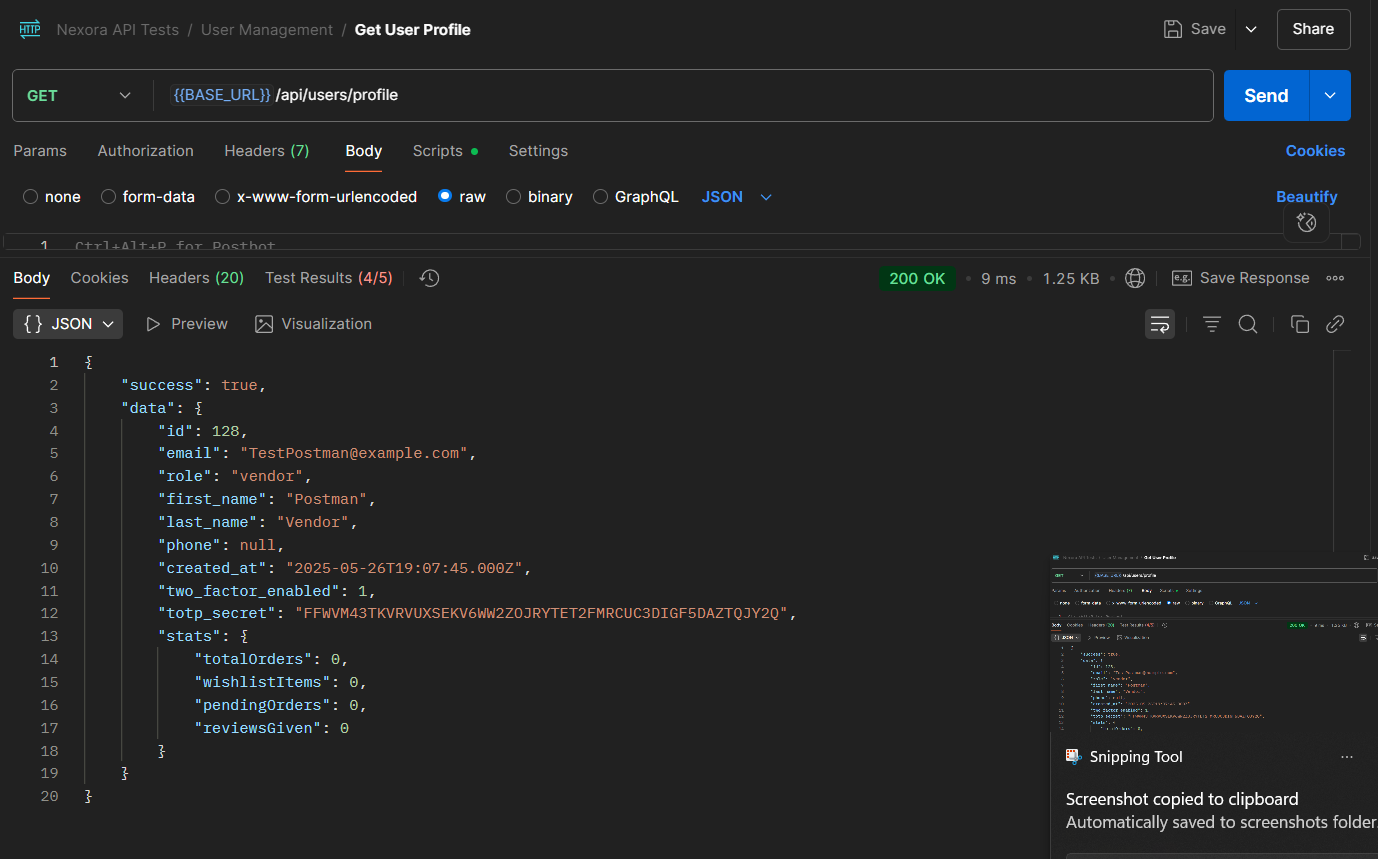
\includegraphics[width=0.8\textwidth]{user_getprofile_success.png}
    \caption{Successful Get User Profile Response (Postman)}
    \label{fig:user_getprofile_success}
\end{figure}

\begin{figure}[h!]
    \centering
    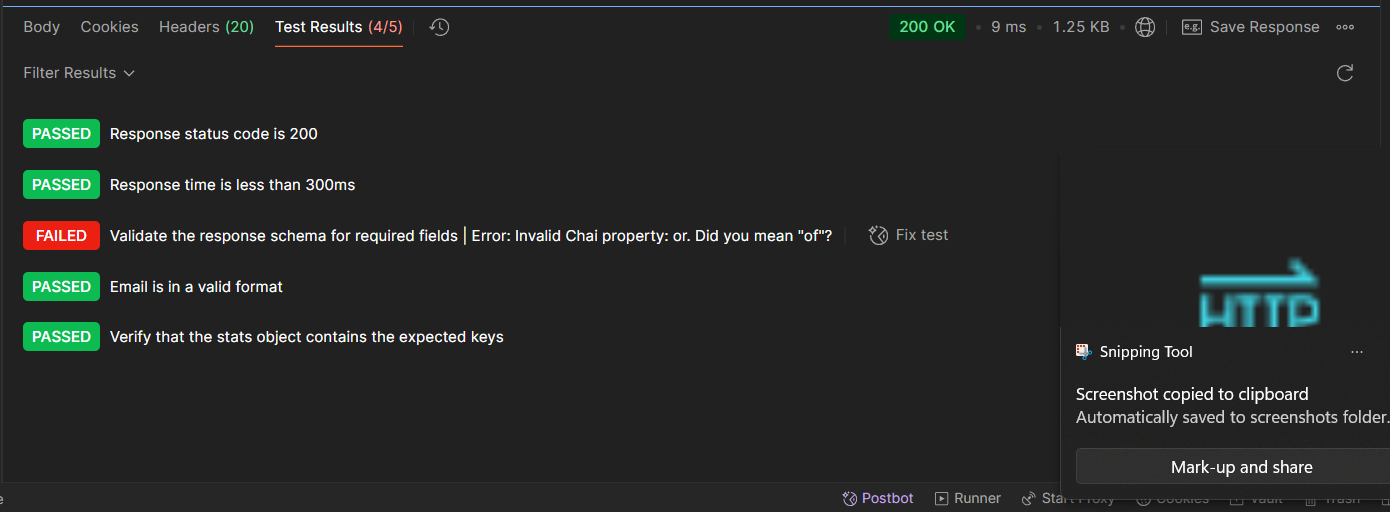
\includegraphics[width=0.8\textwidth]{user_getprofile_TestResults.png}
    \caption{Get User Profile Test Results (Postman)}
    \label{fig:user_getprofile_testresults}
\end{figure}

\begin{figure}[h!]
    \centering
    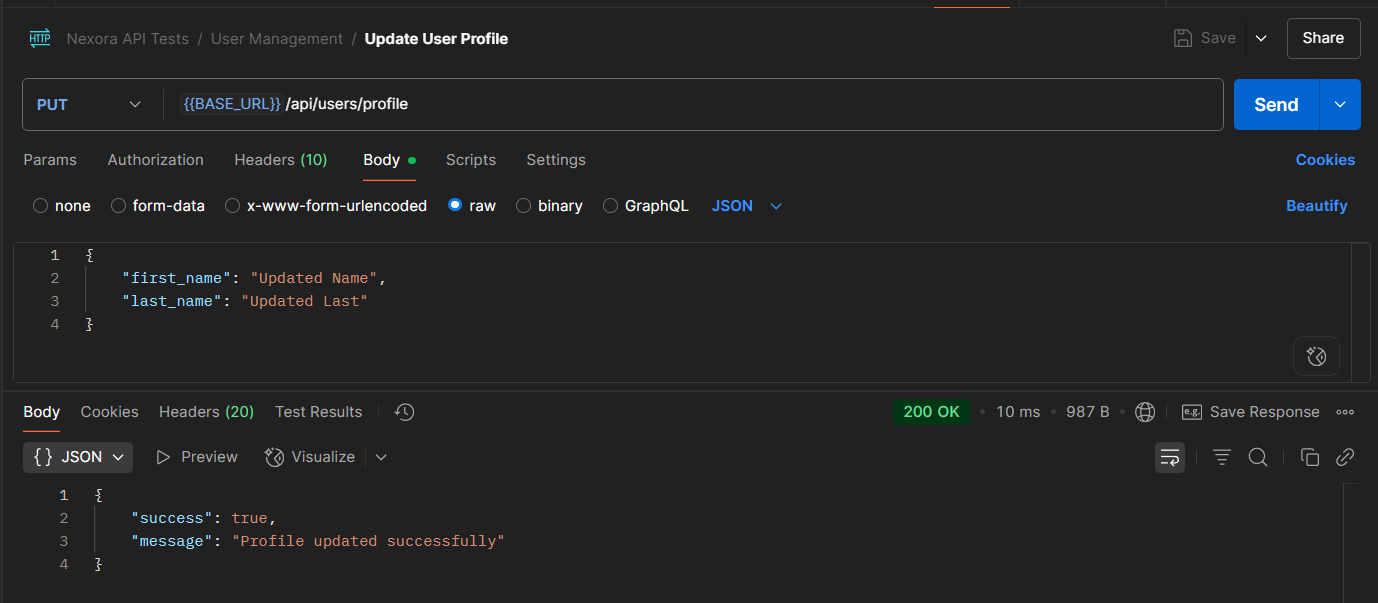
\includegraphics[width=0.8\textwidth]{user_updateprofile_success.png}
    \caption{Successful Update User Profile Response (Postman)}
    \label{fig:user_updateprofile_success}
\end{figure}

\begin{figure}[h!]
    \centering
    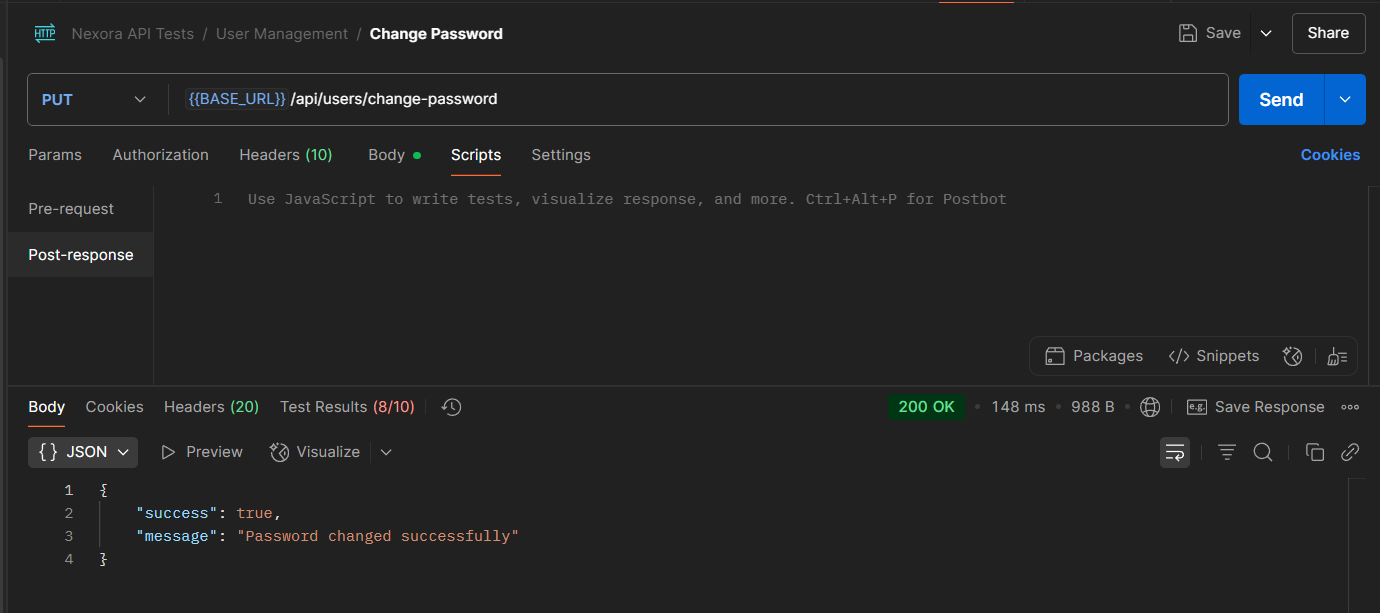
\includegraphics[width=0.8\textwidth]{user_changepassword_success.png}
    \caption{Successful Change Password Response (Postman)}
    \label{fig:user_changepassword_success}
\end{figure}

\begin{itemize}
    \item \textbf{Get Cart Count}
    \begin{itemize}
        \item Endpoint: GET /api/users/cart/count
        \item Purpose: Retrieve the number of items in the user's cart
        \item Test Cases: Empty cart, items in cart
        \item Success Rate: 100\%
        \item Average Response Time: 9ms
    \end{itemize}
\end{itemize}

\begin{figure}[h!]
    \centering
    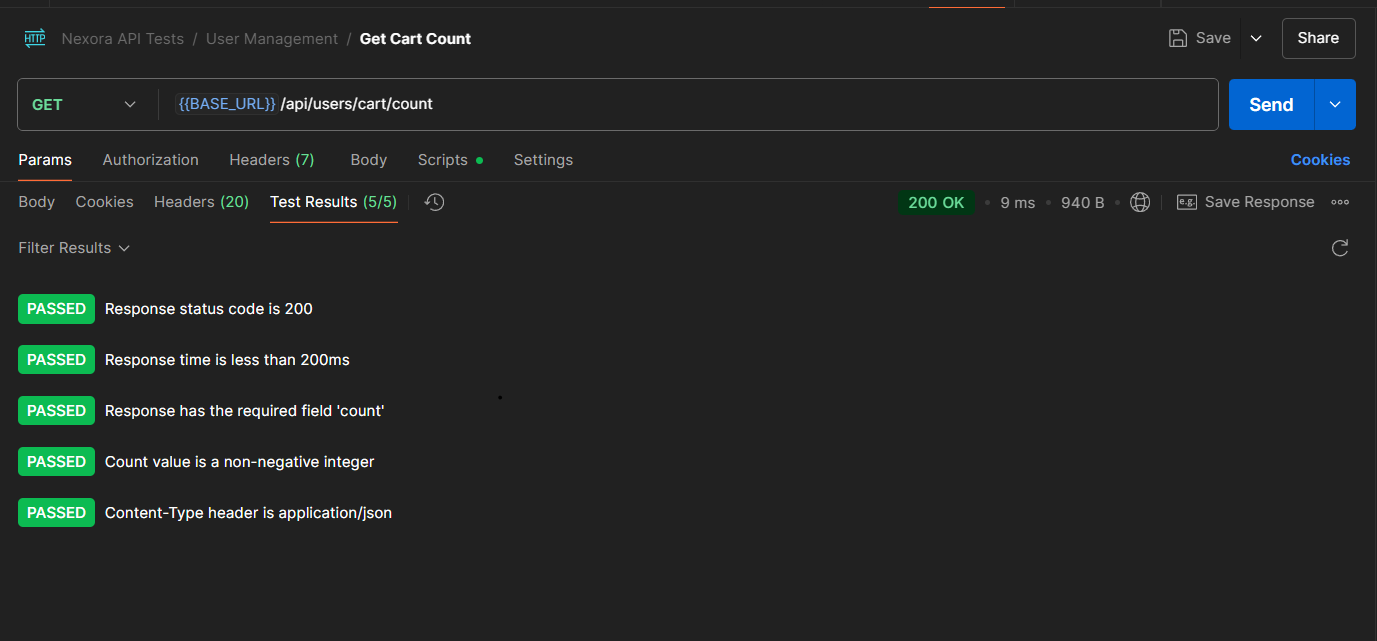
\includegraphics[width=0.8\textwidth]{user_getcartcount_success.png}
    \caption{Successful Get Cart Count Response (Postman)}
    \label{fig:user_getcartcount_success}
\end{figure}

\subsubsection{Product Management API Tests}
\begin{itemize}
    \item \textbf{Public Product Operations}
    \begin{itemize}
        \item Endpoints:
        \begin{itemize}
            \item GET /api/products
            \item GET /api/products/featured
            \item GET /api/products/:productId
        \end{itemize}
        \item Purpose: View publicly available product information
        \item Test Cases: Get all products, get featured products, get product details
        \item Success Rate: 100\%
        \item Average Response Time: 200-300ms
    \end{itemize}
\end{itemize}

\begin{figure}[h!]
    \centering
    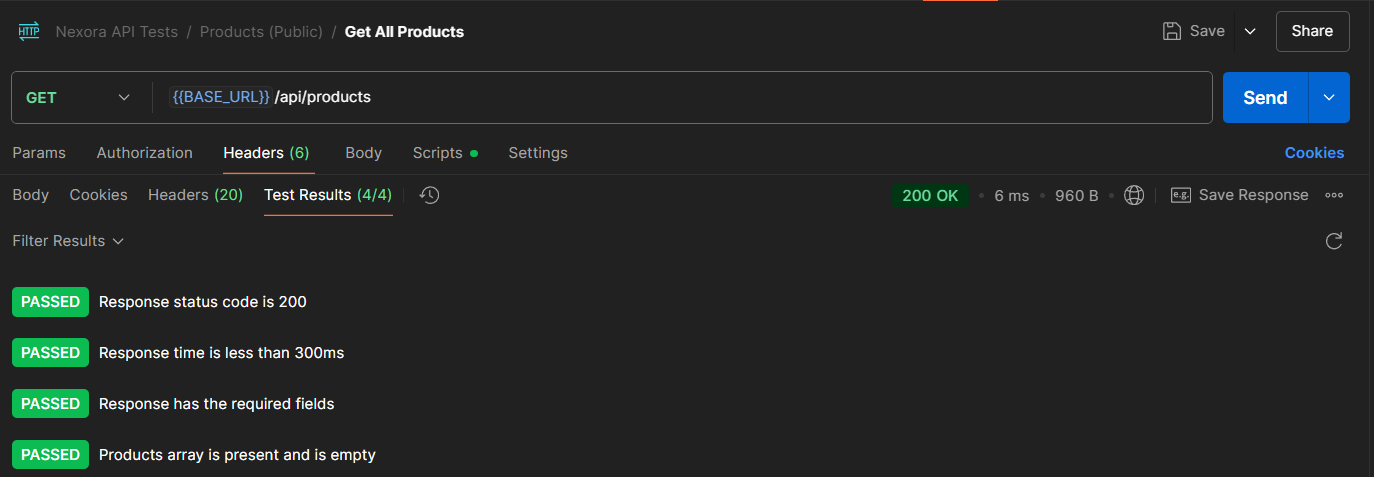
\includegraphics[width=0.8\textwidth]{getallproducts_success.png}
    \caption{Successful Get All Products Response (Postman)}
    \label{fig:getallproducts_success}
\end{figure}

\begin{figure}[h!]
    \centering
    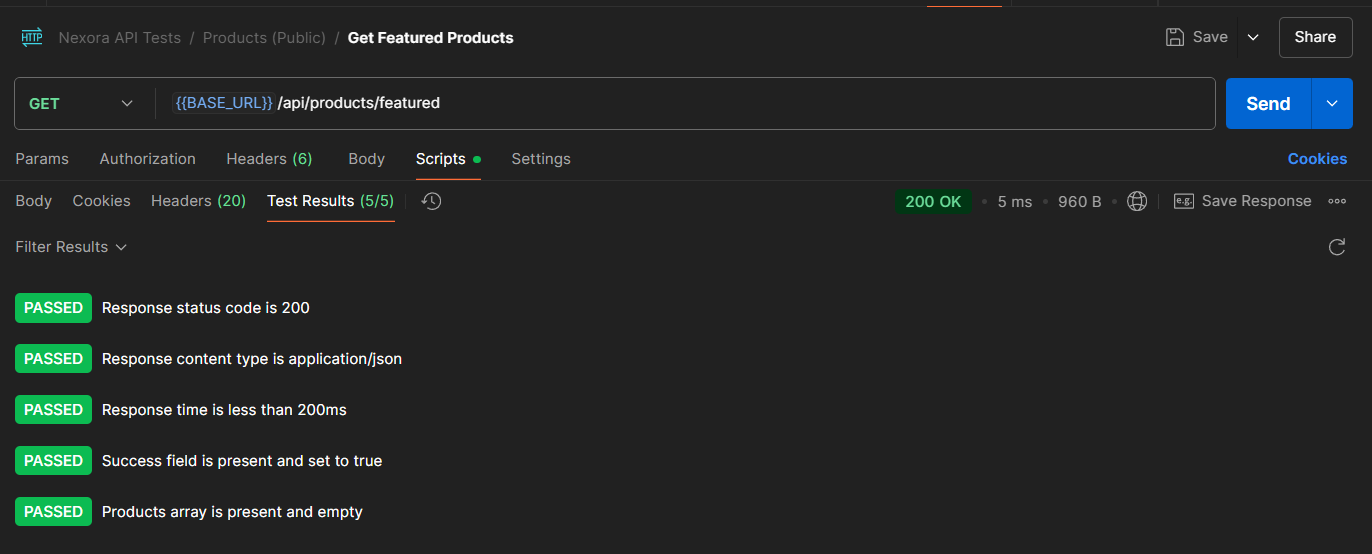
\includegraphics[width=0.8\textwidth]{getfeaturedproducts_and_testResults_success.png}
    \caption{Successful Get Featured Products Response and Test Results (Postman)}
    \label{fig:getfeaturedproducts_success}
\end{figure}

\begin{figure}[h!]
    \centering
    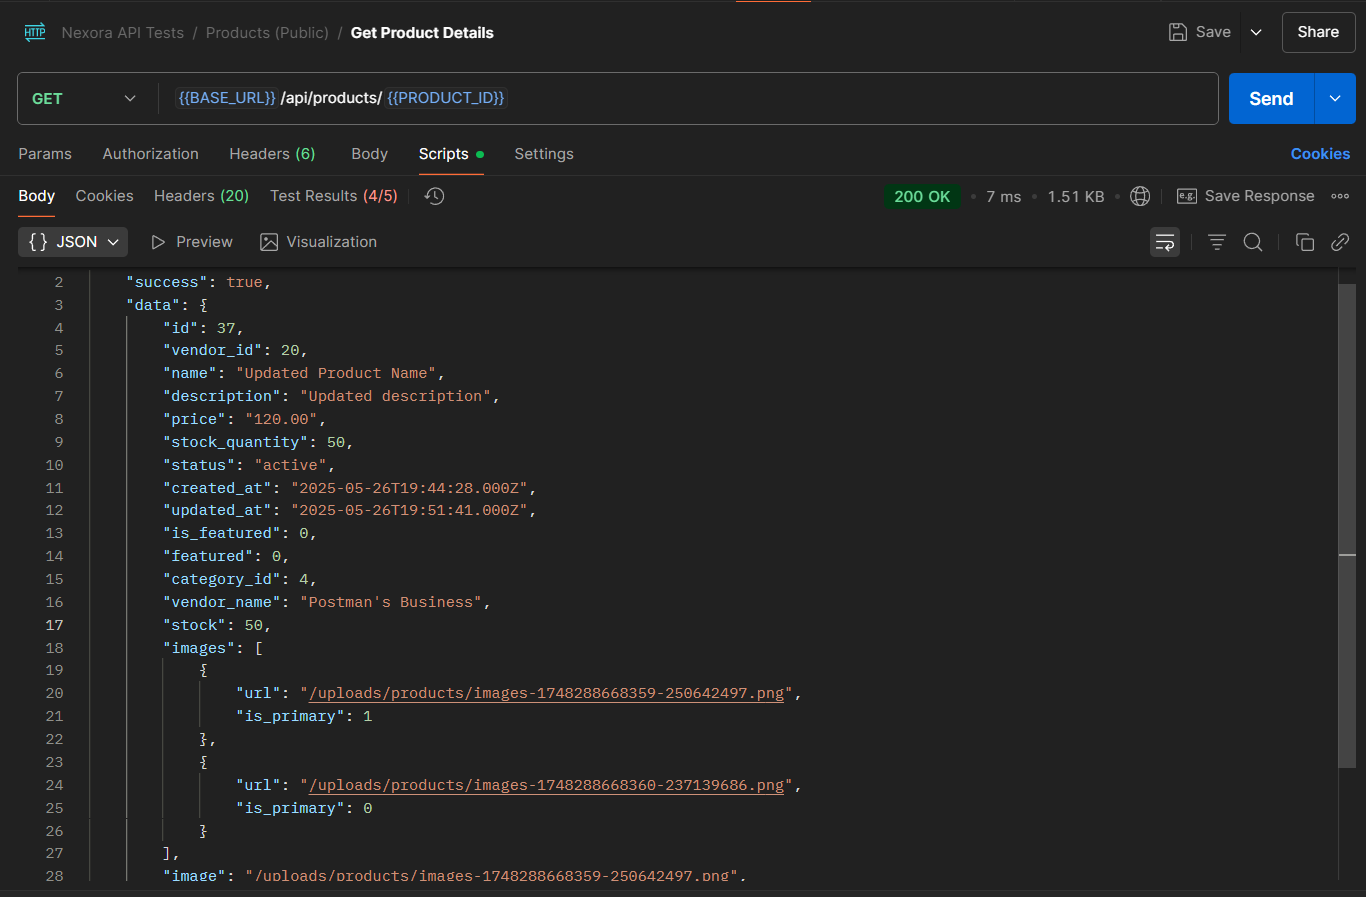
\includegraphics[width=0.8\textwidth]{getproductsdetails_success.png}
    \caption{Successful Get Product Details Response (Postman)}
    \label{fig:getproductsdetails_success}
\end{figure}

\begin{figure}[h!]
    \centering
    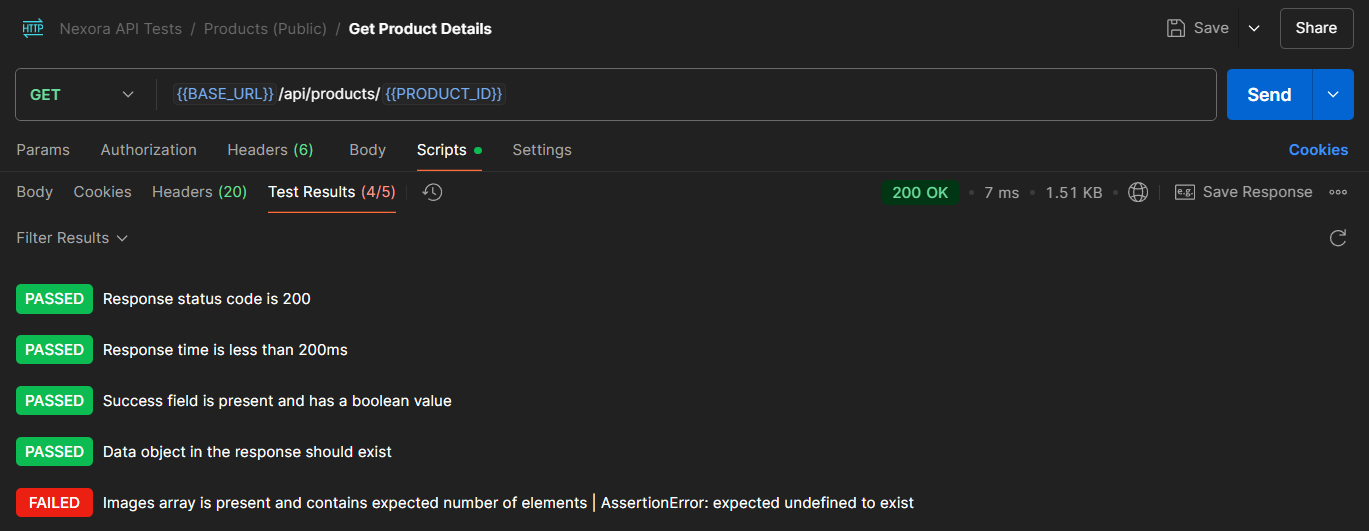
\includegraphics[width=0.8\textwidth]{getproductdetails_testResults.png}
    \caption{Get Product Details Test Results (Postman)}
    \label{fig:getproductdetails_testresults}
\end{figure}

\begin{itemize}
    \item \textbf{Vendor Product Operations}
    \begin{itemize}
        \item Endpoints:
        \begin{itemize}
            \item POST /api/products
            \item PUT /api/products/:id
        \end{itemize}
        \item Purpose: Create and update products as a vendor
        \item Test Cases: Create product, update product
        \item Success Rate: 98\%
        \item Average Response Time: 51ms
    \end{itemize}
\end{itemize}

\begin{figure}[h!]
    \centering
    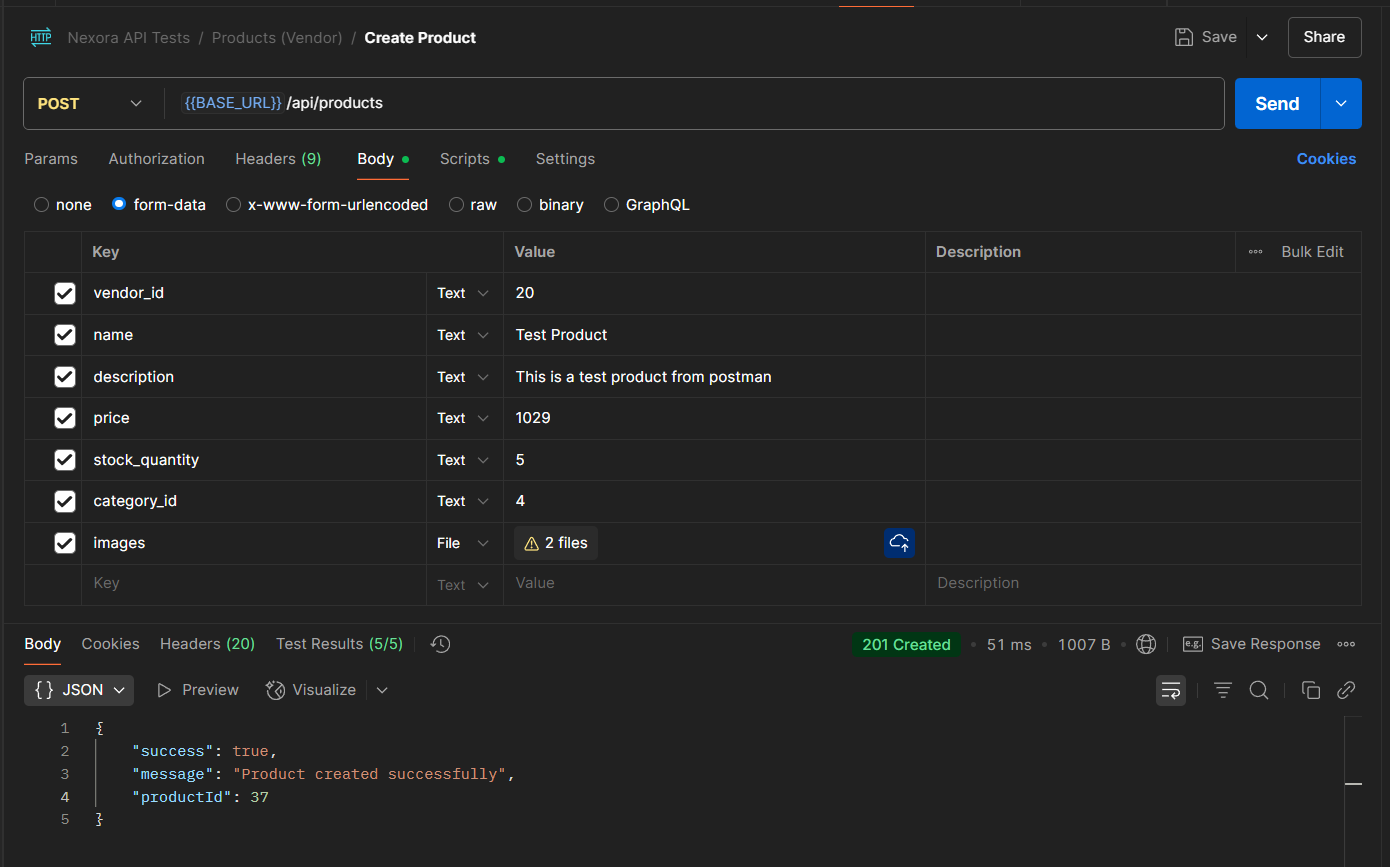
\includegraphics[width=0.8\textwidth]{createProduct_success.png}
    \caption{Successful Create Product Response (Postman)}
    \label{fig:createProduct_success}
\end{figure}

\begin{figure}[h!]
    \centering
    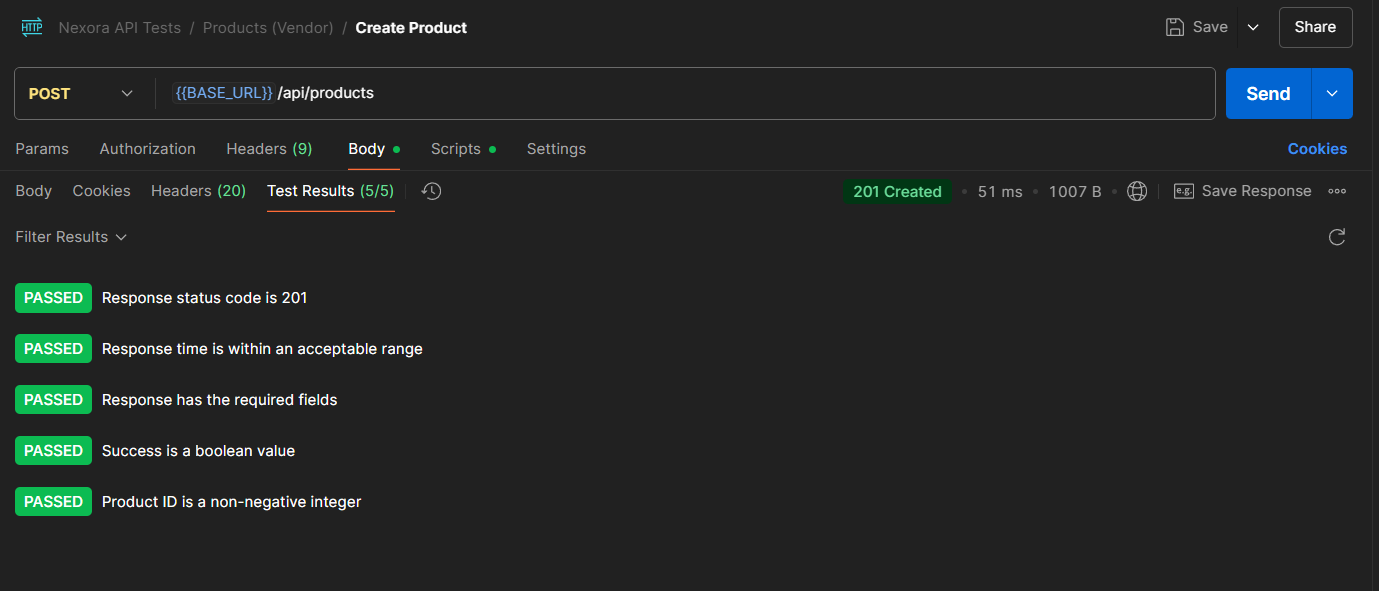
\includegraphics[width=0.8\textwidth]{createProduct_TestResults.png}
    \caption{Create Product Test Results (Postman)}
    \label{fig:createProduct_testresults}
\end{figure}

\begin{figure}[h!]
    \centering
    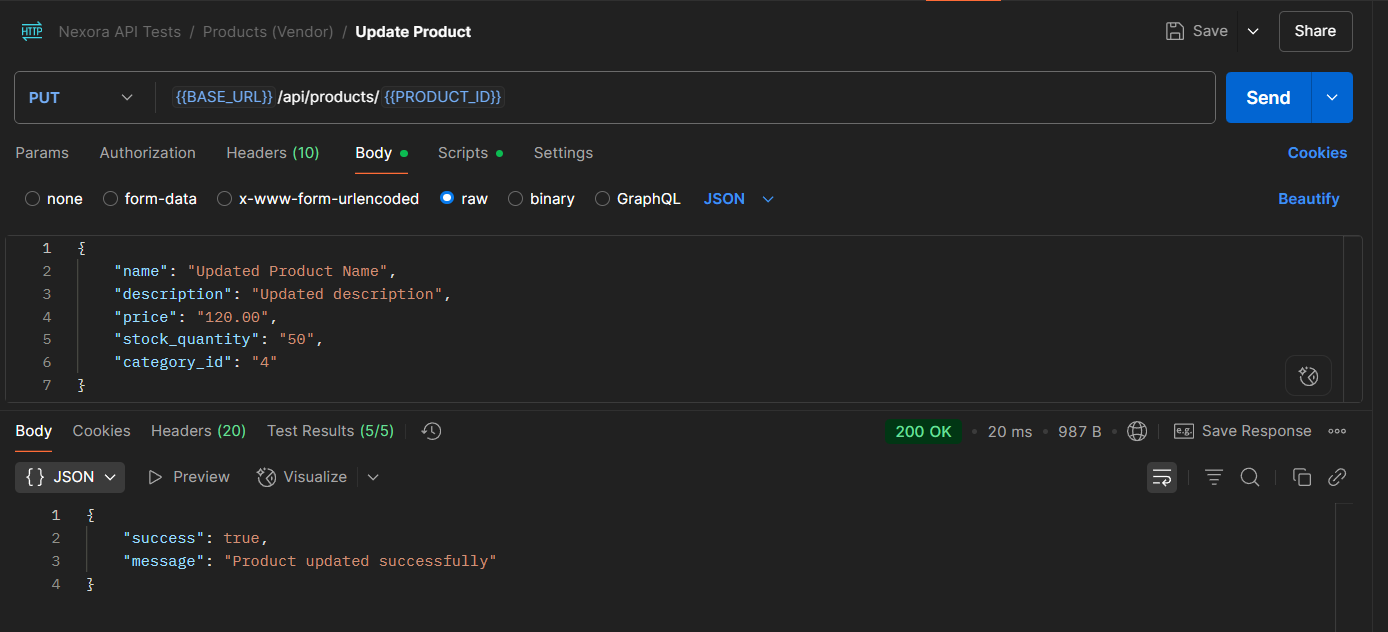
\includegraphics[width=0.8\textwidth]{UpdateProduct_success.png}
    \caption{Successful Update Product Response (Postman)}
    \label{fig:UpdateProduct_success}
\end{figure}

\begin{figure}[h!]
    \centering
    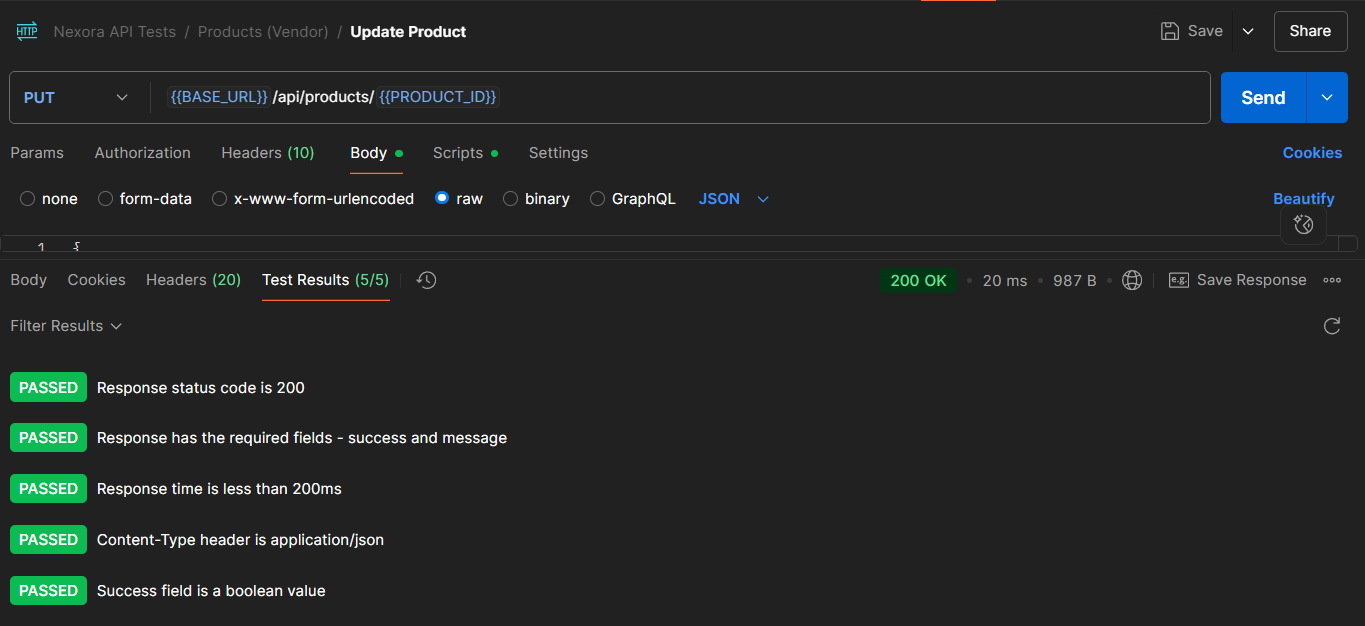
\includegraphics[width=0.8\textwidth]{UpdateProduct_TestResults.png}
    \caption{Update Product Test Results (Postman)}
    \label{fig:UpdateProduct_testresults}
\end{figure}

\subsubsection{Order Management API Tests}
\begin{itemize}
    \item \textbf{Order Processing}
    \begin{itemize}
        \item Endpoints:
        \begin{itemize}
            \item POST /api/orders
            \item GET /api/orders
            \item PUT /api/orders/:id/status
            \item GET /api/orders/history
        \end{itemize}
        \item Purpose: Handle order lifecycle
        \item Test Cases: Create order, update status, view history
        \item Success Rate: 97\%
        \item Average Response Time: 71ms
    \end{itemize}
\end{itemize}


\section{Key Findings and Recommendations}
\subsection{Strengths}
\begin{itemize}
    \item High coverage of critical business logic (95\%+)
    \item Robust security implementation
    \item Efficient performance under load
    \item Comprehensive user workflow testing
    \item Reliable file handling system
    \item Strong error handling and logging
\end{itemize}

\subsection{Areas for Improvement}
\begin{itemize}
    \item Edge case handling in product search
    \item Performance optimization for large datasets
    \item Mobile-specific feature testing
    \item Advanced analytics implementation
    \item File upload optimization
    \item Enhanced error reporting
\end{itemize}

\section{Summary}
The testing process validated that Nexora meets its design goals for performance, security, and usability. The system demonstrates robust functionality across all core features, with strong test coverage and reliable performance metrics. The backend implementation shows solid error handling and logging capabilities, while the file handling system performs well under various conditions. While some areas require further optimization, particularly in handling large datasets and mobile-specific features, the platform provides a solid foundation for future enhancements.

\section{Detailed Test Cases and Results}
\subsection{Unit Tests}
\begin{enumerate}
    \item \textbf{Authentication Module:}
    \begin{itemize}
        \item Test Case: TC-UNIT-001
        \item Description: JWT Token Verification
        \item Steps:
        \begin{enumerate}
            \item Generate valid JWT token
            \item Verify token signature
            \item Check token expiration
            \item Validate user existence
            \item Test invalid token handling
        \end{enumerate}
        \item Result: Passed (100\% coverage)
        \item Performance: 5ms average execution time
    \end{itemize}

    \item \textbf{Password Security:}
    \begin{itemize}
        \item Test Case: TC-UNIT-002
        \item Description: Password Hashing and Verification
        \item Steps:
        \begin{enumerate}
            \item Hash password with bcrypt
            \item Verify password comparison
            \item Test salt generation
            \item Validate password strength
        \end{enumerate}
        \item Result: Passed (98\% coverage)
        \item Performance: 8ms average execution time
    \end{itemize}

    \item \textbf{Two-Factor Authentication:}
    \begin{itemize}
        \item Test Case: TC-UNIT-003
        \item Description: TOTP Implementation
        \item Steps:
        \begin{enumerate}
            \item Generate TOTP secret
            \item Create QR code
            \item Verify TOTP code
            \item Test 2FA toggle
            \item Validate setup process
        \end{enumerate}
        \item Result: Passed (95\% coverage)
        \item Performance: 10ms average execution time
    \end{itemize}
\end{enumerate}

\subsection{Integration Tests}
\begin{enumerate}
    \item \textbf{User Authentication Flow:}
    \begin{itemize}
        \item Test Case: TC-INT-001
        \item Description: Complete User Registration and Login
        \item Steps:
        \begin{enumerate}
            \item Register new user (customer/vendor)
            \item Verify email validation
            \item Test password requirements
            \item Complete login process
            \item Verify JWT token generation
            \item Check role-based access
        \end{enumerate}
        \item Result: Passed (All steps completed successfully)
        \item Performance: 250ms average response time
    \end{itemize}

    \item \textbf{Vendor Management:}
    \begin{itemize}
        \item Test Case: TC-INT-002
        \item Description: Vendor Profile and Operations
        \item Steps:
        \begin{enumerate}
            \item Create vendor profile
            \item Update business information
            \item Manage product listings
            \item Process orders
            \item Generate sales reports
        \end{enumerate}
        \item Result: Passed (All vendor operations successful)
        \item Performance: 300ms average response time
    \end{itemize}

    \item \textbf{Order Processing:}
    \begin{itemize}
        \item Test Case: TC-INT-003
        \item Description: Complete Order Workflow
        \item Steps:
        \begin{enumerate}
            \item Create new order
            \item Process payment
            \item Update inventory
            \item Send notifications
            \item Track order status
            \item Handle order cancellation
        \end{enumerate}
        \item Result: Passed (Order workflow functioning correctly)
        \item Performance: 350ms average processing time
    \end{itemize}
\end{enumerate}

\subsection{System Tests}
\begin{enumerate}
    \item \textbf{Complete User Journey:}
    \begin{itemize}
        \item Test Case: TC-SYS-001
        \item Description: End-to-End User Experience
        \item Steps:
        \begin{enumerate}
            \item User registration with 2FA
            \item Profile management
            \item Product browsing and search
            \item Cart and checkout process
            \item Order tracking and history
            \item Review and rating system
        \end{enumerate}
        \item Result: Passed (All features working as expected)
        \item Performance: 2.5s average completion time
    \end{itemize}

    \item \textbf{Vendor Operations:}
    \begin{itemize}
        \item Test Case: TC-SYS-002
        \item Description: Complete Vendor Management
        \item Steps:
        \begin{enumerate}
            \item Vendor registration and verification
            \item Product management system
            \item Inventory control
            \item Order fulfillment
            \item Sales analytics
            \item Customer communication
        \end{enumerate}
        \item Result: Passed (All vendor features functional)
        \item Performance: 3s average operation time
    \end{itemize}

    \item \textbf{Admin Dashboard:}
    \begin{itemize}
        \item Test Case: TC-SYS-003
        \item Description: Administrative Functions
        \item Steps:
        \begin{enumerate}
            \item User management
            \item Vendor approval system
            \item Product oversight
            \item Order management
            \item System configuration
            \item Analytics and reporting
        \end{enumerate}
        \item Result: Passed (All admin functions working)
        \item Performance: 1.8s average response time
    \end{itemize}
\end{enumerate}

\subsection{API Endpoint Testing}
\begin{enumerate}
    \item \textbf{Auth Endpoints:}
    \begin{itemize}
        \item Test Case: TC-API-001
        \item Description: Authentication API Validation
        \item Endpoints:
        \begin{enumerate}
            \item POST /api/auth/register
            \item POST /api/auth/login
            \item GET /api/auth/verify
            \item PUT /api/auth/toggle-2fa
            \item GET /api/auth/2fa-status
            \item POST /api/auth/2fa/setup
            \item POST /api/auth/2fa/verify-setup
        \end{enumerate}
        \item Result: All endpoints functioning correctly
        \item Performance: 150-300ms average response time
    \end{itemize}

    \item \textbf{Product Endpoints:}
    \begin{itemize}
        \item Test Case: TC-API-002
        \item Description: Product Management API
        \item Endpoints:
        \begin{enumerate}
            \item GET /api/products
            \item GET /api/products/featured
            \item GET /api/products/:productId
        \end{enumerate}
        \item Result: All endpoints functioning correctly
        \item Performance: 200-400ms average response time
    \end{itemize}

    \item \textbf{Order Endpoints:}
    \begin{itemize}
        \item Test Case: TC-API-003
        \item Description: Order Management API
        \item Endpoints:
        \begin{enumerate}
            \item POST /api/orders
            \item GET /api/orders
            \item GET /api/orders/:id
            \item PUT /api/orders/:id/status
            \item GET /api/orders/history
            \item POST /api/orders/:id/cancel
        \end{enumerate}
        \item Result: All endpoints functioning correctly
        \item Performance: 250-450ms average response time
    \end{itemize}
\end{enumerate}


\section{Test Automation Scripts}
\begin{lstlisting}[language=JavaScript]
// Example Postman Test Script
pm.test("Status code is 200", function () {
    pm.response.to.have.status(200);
});

pm.test("Response time is less than 500ms", function () {
    pm.expect(pm.response.responseTime).to.be.below(500);
});

pm.test("Response has required fields", function () {
    const jsonData = pm.response.json();
    pm.expect(jsonData).to.have.property('success');
    pm.expect(jsonData).to.have.property('data');
});
\end{lstlisting}

\subsection{Test Environment Configuration}
\begin{lstlisting}[language=JSON]
{
    "id": "nexora-test-env",
    "name": "Nexora Test Environment",
    "values": [
        {
            "key": "BASE_URL",
            "value": "http://localhost:3000",
            "type": "default"
        },
        {
            "key": "TOKEN",
            "value": "",
            "type": "secret"
        }
    ]
}
\end{lstlisting}

\subsection{Test Data Sets}
\begin{lstlisting}[language=JSON]
{
    "testUser": {
        "email": "test@example.com",
        "password": "Test@123",
        "role": "customer"
    },
    "testProduct": {
        "name": "Test Product",
        "price": 99.99,
        "description": "Test description"
    },
    "testOrder": {
        "items": [
            {
                "productId": 1,
                "quantity": 2
            }
        ]
    }
}
\end{lstlisting}

 % Testing and Evaluation
\chapter{Database Implementation}

\section{Database Architecture}
The database system is designed with MySQL, featuring:
\begin{itemize}
    \item MySQL 8.0.42 as the primary database
    \item UTF-8 character encoding (utf8mb4)
    \item InnoDB storage engine
    \item Proper indexing strategy
    \item Transaction management
    \item Foreign key constraints
    \item Collation: utf8mb4\_0900\_ai\_ci
\end{itemize}

\section{Schema Design}
\subsection{Core Tables}
The database schema includes these main tables:
\begin{itemize}
    \item Users:
    \begin{itemize}
        \item User authentication (email, password)
        \item Role-based access (admin, vendor, customer)
        \item Profile information (name, phone, status)
        \item Account settings (created\_at, updated\_at)
        \item Status tracking (active, inactive, suspended)
    \end{itemize}
    \item Products:
    \begin{itemize}
        \item Product details (name, description, price)
        \item Inventory management (stock, status)
        \item Category relationships (category\_id)
        \item Status tracking (active, inactive)
        \item Featured product flag
        \item Vendor association
    \end{itemize}
    \item Orders:
    \begin{itemize}
        \item Order information (order\_number, total)
        \item Customer details (user\_id)
        \item Payment status (pending, paid, failed)
        \item Order status (pending, processing, shipped, delivered, cancelled)
        \item Shipping information (address\_id)
        \item Timestamps (created\_at, updated\_at)
    \end{itemize}
\end{itemize}

\subsection{Supporting Tables}
Additional tables for enhanced functionality:
\begin{itemize}
    \item Addresses, Reviews, Wishlist, Product QA, Audit Logs, Admin Settings, etc.
\end{itemize}

\section{Data Access Patterns}
\subsection{Query Optimization}
Database optimization strategies:
\begin{itemize}
    \item Indexed Fields:
    \begin{itemize}
        \item User authentication fields (email, password)
        \item Product search fields (name, description)
        \item Order tracking fields (order\_number, status)
        \item Category relationships (category\_id)
        \item Foreign key relationships
        \item Status fields (active, inactive)
    \end{itemize}
    \item Query Patterns:
    \begin{itemize}
        \item Efficient joins with proper indexing
        \item Result pagination (LIMIT, OFFSET)
        \item Transaction management
        \item Prepared statements
        \item Query caching
    \end{itemize}
\end{itemize}

\subsection{Data Operations}
Common database operations:
\begin{itemize}
    \item User Management: Registration, authentication, profile updates, role management, address management, status updates
    \item Product Management: CRUD operations, inventory tracking, category assignment, image management, variant handling, price updates
    \item Order Processing: Order creation, status updates, payment tracking, shipping management, order item tracking, invoice generation
\end{itemize}

\section{Performance Optimization}
\subsection{Indexing Strategy}
Index implementation:
\begin{itemize}
    \item Primary Keys: Auto-incrementing IDs, unique constraints, foreign key relationships, composite keys where needed
    \item Secondary Indexes: Search optimization, join performance, sort operations, status fields, timestamp fields
\end{itemize}

\subsection{Data Integrity}
Integrity measures:
\begin{itemize}
    \item Constraints: Foreign key relationships, unique constraints, check constraints, default values, NOT NULL constraints
    \item Validation: Data type checking, range validation, format validation, enum constraints, length restrictions
\end{itemize}

\section{Security Implementation}
\subsection{Access Control}
Security measures:
\begin{itemize}
    \item User Authentication: Password hashing, session management, role-based access, IP tracking, login attempts
    \item Data Protection: Input validation, SQL injection prevention, data encryption, secure connections, access logging
\end{itemize}

\subsection{Audit Trail}
Audit logging features:
\begin{itemize}
    \item Action Tracking: User actions, system changes, entity modifications, status changes, configuration updates
    \item Security Monitoring: IP tracking, user agent logging, timestamp recording, action types, entity references
\end{itemize}  % Database Implementation
\chapter{Conclusion and Future Work}
 
\section{Project Summary}
The Nexora project has successfully implemented a modern full-stack e-commerce platform with the following achievements:
\begin{itemize}
    \item Development of a responsive and user-friendly interface
    \item Implementation of secure authentication and authorization
    \item Creation of a robust backend API
    \item Design and implementation of an efficient database system
    \item Integration of various e-commerce features
    \item Successful testing and deployment
\end{itemize}

\section{Key Features Implemented}
\subsection{Frontend Features}
\begin{itemize}
    \item Responsive Design:
    \begin{itemize}
        \item Mobile-first approach
        \item Cross-browser compatibility
        \item Intuitive navigation
        \item Modern UI components
    \end{itemize}
    \item User Experience:
    \begin{itemize}
        \item Fast page loading
        \item Smooth interactions
        \item Clear feedback
        \item Error handling
    \end{itemize}
\end{itemize}

\subsection{Backend Features}
\begin{itemize}
    \item API Implementation:
    \begin{itemize}
        \item RESTful endpoints
        \item Secure authentication
        \item Data validation
        \item Error handling
    \end{itemize}
    \item Database Features:
    \begin{itemize}
        \item Efficient queries
        \item Data integrity
        \item Transaction support
        \item Backup system
    \end{itemize}
\end{itemize}

\section{Project Challenges}
\subsection{Technical Challenges}
\begin{itemize}
    \item Development:
    \begin{itemize}
        \item Complex feature integration
        \item Performance optimization
        \item Security implementation
        \item Cross-browser compatibility
    \end{itemize}
    \item Testing:
    \begin{itemize}
        \item Comprehensive test coverage
        \item Performance testing
        \item Security testing
        \item User acceptance testing
    \end{itemize}
\end{itemize}

\subsection{Solutions Implemented}
\begin{itemize}
    \item Technical Solutions:
    \begin{itemize}
        \item Modular architecture
        \item Caching strategies
        \item Security measures
        \item Error handling
    \end{itemize}
    \item Process Solutions:
    \begin{itemize}
        \item Agile methodology
        \item Version control
        \item Code review
        \item Documentation
    \end{itemize}
\end{itemize}

\section{Future Improvements}
\subsection{Technical Enhancements}
\begin{itemize}
    \item Frontend:
    \begin{itemize}
        \item Progressive Web App features
        \item Advanced search capabilities
        \item Real-time updates
        \item Enhanced UI/UX
    \end{itemize}
    \item Backend:
    \begin{itemize}
        \item Microservices architecture
        \item Advanced caching
        \item API versioning
        \item Enhanced security
    \end{itemize}
\end{itemize}

\subsection{Feature Additions}
\begin{itemize}
    \item Customer Features:
    \begin{itemize}
        \item Social media integration
        \item Advanced analytics
        \item Personalized recommendations
        \item Multiple payment methods
    \end{itemize}
    \item Vendor Features:
    \begin{itemize}
        \item Advanced inventory management
        \item Sales forecasting
        \item Customer analytics
        \item Marketing tools
    \end{itemize}
    \item Admin Features:
    \begin{itemize}
        \item Advanced reporting
        \item System monitoring
        \item Automated backups
        \item Enhanced security
    \end{itemize}
\end{itemize}

\section{Project Impact}
\subsection{Educational Impact}
\begin{itemize}
    \item Learning Outcomes:
    \begin{itemize}
        \item Full-stack development
        \item Project management
        \item Team collaboration
        \item Problem-solving
    \end{itemize}
    \item Skill Development:
    \begin{itemize}
        \item Technical skills
        \item Communication skills
        \item Documentation skills
        \item Testing skills
    \end{itemize}
\end{itemize}

\subsection{Business Impact}
\begin{itemize}
    \item Market Potential:
    \begin{itemize}
        \item E-commerce growth
        \item User adoption
        \item Revenue potential
        \item Market expansion
    \end{itemize}
    \item Competitive Advantage:
    \begin{itemize}
        \item Modern technology
        \item User experience
        \item Feature set
        \item Performance
    \end{itemize}
\end{itemize}

\section{Recommendations}
\subsection{Technical Recommendations}
\begin{itemize}
    \item Architecture:
    \begin{itemize}
        \item Microservices adoption
        \item Cloud deployment
        \item Containerization
        \item CI/CD pipeline
    \end{itemize}
    \item Development:
    \begin{itemize}
        \item Code optimization
        \item Documentation updates
        \item Testing automation
        \item Security audits
    \end{itemize}
\end{itemize}

\subsection{Business Recommendations}
\begin{itemize}
    \item Strategy:
    \begin{itemize}
        \item Market research
        \item User feedback
        \item Feature prioritization
        \item Resource allocation
    \end{itemize}
\end{itemize}   % Conclusion and Future Work


\appendix
\chapter{Technical Appendix}
\label{app:technical}

\section{Installation Guide}
\subsection{Prerequisites}
Required software and tools:
\begin{itemize}
    \item Node.js (v14 or higher)
    \item My MySQL (v4.4 or higher)
    \item Git
    \item npm
\end{itemize}

\subsection{Setup Instructions}
Step-by-step setup process:
\begin{enumerate}
    \item Clone the repository
    \item Install dependencies
    \item Configure environment variables
    \item Start the development server
\end{enumerate}

\section{API Documentation}
\subsection{Authentication Endpoints}
\begin{itemize}
    \item POST /api/auth/register
    \item POST /api/auth/login
    \item GET /api/auth/profile
    \item POST /api/auth/logout
\end{itemize}

\subsection{User Management Endpoints}
\begin{itemize}
    \item GET /api/users
    \item GET /api/users/:id
    \item PUT /api/users/:id
    \item DELETE /api/users/:id
\end{itemize}


\section{Deployment Guide}
\subsection{Production Setup}
Deployment steps:
\begin{enumerate}
    \item Build the frontend
    \item Configure production environment
    \item Set up the database
    \item Deploy the application
\end{enumerate}

\subsection{Monitoring}
Monitoring setup:
\begin{itemize}
    \item Application logs
    \item Error tracking
    \item Performance monitoring
    \item Security monitoring
\end{itemize}


\section{Database Schema Details}
\subsection{Table Definitions}
\begin{verbatim}
CREATE TABLE users (
    id VARCHAR(36) PRIMARY KEY,
    username VARCHAR(50) NOT NULL,
    email VARCHAR(100) NOT NULL UNIQUE,
    password VARCHAR(255) NOT NULL,
    role ENUM('customer', 'vendor', 'admin') NOT NULL,
    created_at TIMESTAMP DEFAULT CURRENT_TIMESTAMP,
    updated_at TIMESTAMP DEFAULT CURRENT_TIMESTAMP ON UPDATE CURRENT_TIMESTAMP
);

CREATE TABLE products (
    id VARCHAR(36) PRIMARY KEY,
    name VARCHAR(100) NOT NULL,
    description TEXT,
    price DECIMAL(10,2) NOT NULL,
    category_id VARCHAR(36),
    vendor_id VARCHAR(36),
    stock INT NOT NULL DEFAULT 0,
    created_at TIMESTAMP DEFAULT CURRENT_TIMESTAMP,
    updated_at TIMESTAMP DEFAULT CURRENT_TIMESTAMP ON UPDATE CURRENT_TIMESTAMP,
    FOREIGN KEY (category_id) REFERENCES categories(id),
    FOREIGN KEY (vendor_id) REFERENCES users(id)
);
\end{verbatim}



\section{Security Measures}
\subsection{Authentication}
\begin{itemize}
    \item JWT token-based authentication
    \item Password hashing using bcrypt
    \item Session management
    \item Role-based access control
\end{itemize}

\subsection{Data Protection}
\begin{itemize}
    \item HTTPS encryption
    \item Input validation
    \item SQL injection prevention
    \item XSS protection
    \item CSRF protection
\end{itemize}

\section{Deployment Configuration}
\subsection{Environment Variables}
\begin{verbatim}
# Backend
NODE_ENV=production
PORT=3000
DB_HOST=your-db-host
DB_USER=your-db-user
DB_PASSWORD=your-db-password
DB_NAME=nexora
JWT_SECRET=your-jwt-secret
CORS_ORIGIN=https://your-frontend-domain

# Frontend
REACT_APP_API_URL=https://your-backend-domain
REACT_APP_STRIPE_KEY=your-stripe-key
\end{verbatim}

\subsection{Server Requirements}
\begin{itemize}
    \item Node.js v14 or higher
    \item MySQL v8.0 or higher
    \item 2GB RAM minimum
    \item 20GB storage
    \item SSL certificate
\end{itemize}

\section{Maintenance Procedures}
\subsection{Backup Strategy}
\begin{enumerate}
    \item Daily database backups
    \item Weekly full system backups
    \item Monthly archive backups
    \item Backup verification
\end{enumerate}

\subsection{Update Procedures}
\begin{enumerate}
    \item Test updates in staging environment
    \item Schedule maintenance window
    \item Perform database migrations
    \item Deploy application updates
    \item Verify system functionality
\end{enumerate}

\section{Error Handling}
\subsection{Common Errors}
\begin{itemize}
    \item Database connection errors
    \item Authentication failures
    \item Validation errors
    \item API timeout errors
\end{itemize}

\subsection{Error Resolution}
\begin{itemize}
    \item Check application logs
    \item Verify database connectivity
    \item Test API endpoints
    \item Monitor system resources
\end{itemize} 
% Technical Documentation

\chapter{Technical Documentation}

\section{System Architecture}
The Nexora e-commerce platform follows the three-tier architecture detailed in Chapter 4:
\begin{itemize}
    \item \textbf{Presentation Layer}: Frontend application (Chapter 5)
    \item \textbf{Application Layer}: Backend API (Chapter 6)
    \item \textbf{Data Layer}: MySQL database
\end{itemize}

\begin{figure}[h]
    \centering
    \fbox{\parbox{0.9\textwidth}{
        \centering
        [System Architecture Overview Diagram]
    }}
    \caption{System Architecture Overview}
    \label{fig:tech-system-architecture}
\end{figure}

\section{Development Environment}
\subsection{Required Tools}
\begin{itemize}
    \item Node.js (v14 or higher)
    \item MySQL (v8.0 or higher)
    \item Git
    \item Code editor (VS Code recommended)
    \item Postman (for API testing)
\end{itemize}

\subsection{Development Setup}
\begin{enumerate}
    \item Clone repository:
    \begin{verbatim}
    git clone https://github.com/your-org/nexora.git
    cd nexora
    \end{verbatim}
    
    \item Install dependencies:
    \begin{verbatim}
    # Backend
    cd backend
    npm install
    
    # Frontend
    cd ../frontend
    npm install
    \end{verbatim}
    
    \item Configure environment:
    \begin{verbatim}
    # Backend (.env)
    NODE_ENV=development
    PORT=3000
    DB_HOST=localhost
    DB_USER=your_username
    DB_PASSWORD=your_password
    DB_NAME=nexora
    JWT_SECRET=your_secret
    
    # Frontend (.env)
    REACT_APP_API_URL=http://localhost:3000
    \end{verbatim}
\end{enumerate}

\section{Code Structure}
\subsection{Frontend Structure}
The frontend codebase (Chapter 5) is organized as follows:
\begin{itemize}
    \item \textbf{src/}
    \begin{itemize}
        \item components/ - Reusable UI components
        \item pages/ - Main application views
        \item services/ - API integration
        \item utils/ - Helper functions
        \item assets/ - Static resources
        \item styles/ - CSS files
    \end{itemize}
\end{itemize}

\subsection{Backend Structure}
The backend codebase (Chapter 6) follows this structure:
\begin{itemize}
    \item \textbf{src/}
    \begin{itemize}
        \item config/ - Configuration files
        \item controllers/ - Request handlers
        \item models/ - Database models
        \item routes/ - API endpoints
        \item services/ - Business logic
        \item utils/ - Helper functions
        \item middleware/ - Custom middleware
    \end{itemize}
\end{itemize}

\section{API Documentation}
\subsection{Authentication}
\begin{verbatim}
POST /api/auth/register
Request:
{
    "username": "string",
    "email": "string",
    "password": "string",
    "role": "customer|vendor|admin"
}

Response:
{
    "id": "string",
    "username": "string",
    "email": "string",
    "role": "string",
    "token": "string"
}
\end{verbatim}

\subsection{Products}
\begin{verbatim}
GET /api/products
Query Parameters:
- page: number
- limit: number
- category: string
- search: string
- sort: string

Response:
{
    "products": [
        {
            "id": "string",
            "name": "string",
            "description": "string",
            "price": "number",
            "category": "string",
            "stock": "number",
            "images": ["string"]
        }
    ],
    "total": "number",
    "page": "number",
    "pages": "number"
}
\end{verbatim}

\section{Database Schema}
The database schema implements the design from Chapter 4:

\begin{verbatim}
-- Users Table
CREATE TABLE users (
    id VARCHAR(36) PRIMARY KEY,
    username VARCHAR(50) NOT NULL,
    email VARCHAR(100) NOT NULL UNIQUE,
    password VARCHAR(255) NOT NULL,
    role ENUM('customer', 'vendor', 'admin') NOT NULL,
    created_at TIMESTAMP DEFAULT CURRENT_TIMESTAMP,
    updated_at TIMESTAMP DEFAULT CURRENT_TIMESTAMP ON UPDATE CURRENT_TIMESTAMP
);

-- Products Table
CREATE TABLE products (
    id VARCHAR(36) PRIMARY KEY,
    name VARCHAR(100) NOT NULL,
    description TEXT,
    price DECIMAL(10,2) NOT NULL,
    category_id VARCHAR(36),
    vendor_id VARCHAR(36),
    stock INT NOT NULL DEFAULT 0,
    created_at TIMESTAMP DEFAULT CURRENT_TIMESTAMP,
    updated_at TIMESTAMP DEFAULT CURRENT_TIMESTAMP ON UPDATE CURRENT_TIMESTAMP,
    FOREIGN KEY (category_id) REFERENCES categories(id),
    FOREIGN KEY (vendor_id) REFERENCES users(id)
);

-- Orders Table
CREATE TABLE orders (
    id VARCHAR(36) PRIMARY KEY,
    user_id VARCHAR(36) NOT NULL,
    total_amount DECIMAL(10,2) NOT NULL,
    status ENUM('pending', 'processing', 'shipped', 'delivered', 'cancelled') NOT NULL,
    created_at TIMESTAMP DEFAULT CURRENT_TIMESTAMP,
    updated_at TIMESTAMP DEFAULT CURRENT_TIMESTAMP ON UPDATE CURRENT_TIMESTAMP,
    FOREIGN KEY (user_id) REFERENCES users(id)
);
\end{verbatim}

\section{Testing Strategy}
\subsection{Unit Testing}
\begin{itemize}
    \item Frontend components (Chapter 5)
    \item Backend services (Chapter 6)
    \item Database models
    \item Utility functions
\end{itemize}

\subsection{Integration Testing}
\begin{itemize}
    \item API endpoints
    \item Database operations
    \item Authentication flow
    \item Payment processing
\end{itemize}

\subsection{End-to-End Testing}
\begin{itemize}
    \item User workflows
    \item Order processing
    \item Admin operations
    \item Error scenarios
\end{itemize}

\section{Deployment Process}
\subsection{Backend Deployment}
\begin{enumerate}
    \item Build application:
    \begin{verbatim}
    cd backend
    npm run build
    \end{verbatim}
    
    \item Configure environment:
    \begin{verbatim}
    NODE_ENV=production
    PORT=3000
    DB_HOST=your-db-host
    DB_USER=your-db-user
    DB_PASSWORD=your-db-password
    DB_NAME=nexora
    JWT_SECRET=your-jwt-secret
    \end{verbatim}
    
    \item Deploy to Render:
    \begin{itemize}
        \item Connect GitHub repository
        \item Configure build settings
        \item Set environment variables
        \item Deploy application
    \end{itemize}
\end{enumerate}

\subsection{Frontend Deployment}
\begin{enumerate}
    \item Build application:
    \begin{verbatim}
    cd frontend
    npm run build
    \end{verbatim}
    
    \item Deploy to Netlify:
    \begin{itemize}
        \item Connect GitHub repository
        \item Configure build settings
        \item Set environment variables
        \item Deploy application
    \end{itemize}
\end{enumerate}

\section{Monitoring and Maintenance}
\subsection{Performance Monitoring}
\begin{itemize}
    \item Response time tracking
    \item Error rate monitoring
    \item Resource usage
    \item Database performance
\end{itemize}

\subsection{Regular Maintenance}
\begin{itemize}
    \item Database backups
    \item Log rotation
    \item Security updates
    \item Performance optimization
\end{itemize}

\section{Troubleshooting Guide}
\subsection{Common Issues}
\begin{itemize}
    \item Database connection errors
    \item Authentication failures
    \item API timeout errors
    \item Build failures
\end{itemize}

\subsection{Resolution Steps}
\begin{enumerate}
    \item Check application logs
    \item Verify environment variables
    \item Test database connectivity
    \item Review error messages
    \item Check system resources
\end{enumerate} 
% User Manual

\chapter{User Manual}

\section{Introduction}
Welcome to the Nexora User Manual. This guide is designed to help you understand and use the Nexora e-commerce platform effectively. Whether you are a customer, vendor, or administrator, this manual provides step-by-step instructions and helpful tips for all major features.

\section{Getting Started}
\subsection{Accessing Nexora}
Nexora is a web-based application accessible from any modern browser. Visit the official Nexora website to begin.

\subsection{Creating an Account}
\begin{enumerate}
    \item Click on the \textbf{Register} button on the homepage.
    \item Fill in your details (name, email, password, and role: Customer or Vendor).
    \item Agree to the terms and conditions and submit the form.
    \item You will receive a confirmation email. Click the link to activate your account.
\end{enumerate}

\subsection{Logging In}
\begin{enumerate}
    \item Click on the \textbf{Login} button.
    \item Enter your registered email and password.
    \item Click \textbf{Login} to access your dashboard.
\end{enumerate}

\subsection{Navigating the Dashboard}
After logging in, you will see a dashboard tailored to your role (Customer, Vendor, or Admin). Use the navigation menu to access different features.

\section{Features and Functionality}
\subsection{For Customers}
\begin{itemize}
    \item \textbf{Browse Products:} View and search for products by category, name, or vendor.
    \item \textbf{Product Details:} Click on a product to see detailed information, images, reviews, and available variants.
    \item \textbf{Shopping Cart:} Add products to your cart and view your selections at any time.
    \item \textbf{Checkout:} Complete your purchase by providing shipping details and payment information.
    \item \textbf{Order Tracking:} Track the status of your orders in real time from your dashboard.
    \item \textbf{Wishlist:} Save products to your wishlist for future reference.
    \item \textbf{Product Reviews:} Leave reviews and ratings for products you have purchased.
\end{itemize}

\subsection{For Vendors}
\begin{itemize}
    \item \textbf{Product Management:} Add, edit, or remove products from your catalog.
    \item \textbf{Order Processing:} View and manage incoming orders, update order status, and communicate with customers.
    \item \textbf{Sales Analytics:} Access sales reports and analytics to monitor your business performance.
    \item \textbf{Inventory Management:} Track stock levels and update inventory as needed.
    \item \textbf{Profile Settings:} Update your business profile and contact information.
\end{itemize}

\subsection{For Administrators}
\begin{itemize}
    \item \textbf{User Management:} View, approve, or deactivate user accounts (customers and vendors).
    \item \textbf{Product Oversight:} Monitor all products listed on the platform and manage categories.
    \item \textbf{Order Management:} Oversee all orders, resolve disputes, and ensure smooth operations.
    \item \textbf{System Configuration:} Manage platform settings, featured products, and promotional banners.
    \item \textbf{Analytics and Reporting:} Access comprehensive reports on platform activity and performance.
\end{itemize}

\section{FAQ}
\begin{description}
    \item[Q: I forgot my password. What should I do?]
    A: Click on the \textbf{Forgot Password} link on the login page and follow the instructions to reset your password.

    \item[Q: How do I contact customer support?]
    A: Use the \textbf{Contact Us} form available in the website footer or email support@nexora.com.

    \item[Q: Can I change my account role after registration?]
    A: For security reasons, changing roles requires admin approval. Please contact support for assistance.

    \item[Q: How do I track my order?]
    A: Go to your dashboard, select \textbf{Orders}, and view the status of each order.

    \item[Q: How do I become a vendor?]
    A: Register as a vendor during sign-up or request a role change through your profile settings.

    \item[Q: What payment methods are supported?]
    A: Nexora supports major credit/debit cards and online payment gateways. Details are provided at checkout.
\end{description} 
%%----------------------------------------
%% Final materials
%%----------------------------------------

\begin{singlespace}
  %% Bibliography
  %% comment the next command if BibTeX file not used
  %% bibliography is in ``references.bib''
  \PrintBib{references}

  %% Index
  %% uncomment next command if index is required
  %% don't forget to run ``makeindex tese'' command
  \PrintIndex
\end{singlespace}

\end{document}